%File: anonymous-submission-latex-2024.tex
\documentclass[letterpaper]{article} % DO NOT CHANGE THIS
\usepackage[submission]{aaai24}  % DO NOT CHANGE THIS
\usepackage{times}  % DO NOT CHANGE THIS
\usepackage{helvet}  % DO NOT CHANGE THIS
\usepackage{courier}  % DO NOT CHANGE THIS
\usepackage[hyphens]{url}  % DO NOT CHANGE THIS
\usepackage{graphicx} % DO NOT CHANGE THIS
\urlstyle{rm} % DO NOT CHANGE THIS
\def\UrlFont{\rm}  % DO NOT CHANGE THIS
\usepackage{natbib}  % DO NOT CHANGE THIS AND DO NOT ADD ANY OPTIONS TO IT
\usepackage{caption} % DO NOT CHANGE THIS AND DO NOT ADD ANY OPTIONS TO IT
\frenchspacing  % DO NOT CHANGE THIS
\setlength{\pdfpagewidth}{8.5in} % DO NOT CHANGE THIS
\setlength{\pdfpageheight}{11in} % DO NOT CHANGE THIS
%
% These are recommended to typeset algorithms but not required. See the subsubsection on algorithms. Remove them if you don't have algorithms in your paper.
\usepackage{amsmath}
\usepackage{amsthm}
\usepackage{amssymb}
\usepackage{booktabs}
\usepackage{algorithm}
\usepackage{algpseudocode}
\usepackage[smaller]{acronym}
\usepackage{xspace}
\usepackage{listings, xcolor}

\usepackage{adjustbox}
\usepackage{subcaption}
\usepackage{paralist}
\usepackage{fancyvrb}
% \usepackage{xr}

% \makeatletter


\newfloat{lstfloat}{htbp}{lop}
\floatname{lstfloat}{Listing}

\newcommand{\safe}{\textit{safe}}
\newcommand{\conflict}{\textit{conflict}}
\newcommand{\pre}{\textit{pre}}
\newcommand{\eff}{\textit{eff}}
\newcommand{\add}{\textit{add}}
\newcommand{\del}{\textit{del}}
\newcommand{\post}{\textit{post}}
\newcommand{\fail}{\textit{fail}}
\newcommand{\public}{\textit{public}}
\newcommand{\private}{\textit{private}}
\newcommand{\pol}{\ac{POL}\xspace}
\newcommand{\epol}{\ac{EPOL}\xspace}
\newcommand{\cmapbb}{\ac{CMAP-BB}\xspace}
\theoremstyle{definition}
\newtheorem{definition}{Definition}
\newtheorem{theorem}{Theorem}
\newtheorem{lemma}[theorem]{Lemma}
\newtheorem{corollary}[theorem]{Corollary}
\theoremstyle{remark}
\newtheorem*{remark}{Remark}
\newtheorem{observation}{Observation}

\newcommand{\tuple}[1]{\ensuremath{\left \langle #1 \right \rangle }}
\newcommand{\params}{\textit{params}}
\newcommand{\objects}{\textit{objects}}
\newcommand{\lifted}{\textit{lifted}}
\newcommand{\relevant}{\textit{relevant}}


\newcommand{\name}{\textit{name}}
\newcommand{\type}{\textit{type}}
\newcommand{\cnf}{\textit{CNF}}
\newcommand{\conj}{\textit{Conj}}
\newcommand{\realm}{\ensuremath{M^*}\xspace}
\newcommand{\liftf}{\mathsf{f}}
% \newcommand{\liftl}{\mathsf{l}} RONI: This looks too much like "one"
\newcommand{\liftl}{\ensuremath{\ell}}
\newcommand{\lifta}{\mathsf{a}}
\newcommand{\liftatag}{\mathsf{a}'}
\newcommand{\esam}{\textit{ESAM}\xspace}
\newcommand{\sgam}{\textit{SGAM}\xspace}
\newcommand{\bindings}{\textit{bindings}}
\newcommand{\iseff}{\text{IsEff}}
\newcommand{\ispre}{\text{IsPre}}

\acrodef{NO-OP}{No Operation}
\acrodef{CMAP-BB}{CMAP with Black-Box Agents}
\acrodef{MF-MAP}{Model-Free Multi-Agent Planning}
\acrodef{MA-SAM}{Multi-Agent Safe Action Model Learning}
\acrodef{SAM}{Safe Action Model Learning}
\acrodef{JAT}{Joint Action Trajectory}
\acrodef{LMA}{Lifted Macro Action}
% \newcommand{\noop}{\ac{NO-OP}\xspace}
\newcommand{\noop}{\textit{NO-OP}\xspace}
\newcommand{\sam}{\ac{SAM}\xspace}
\newcommand{\masam}{\ac{MA-SAM}\xspace}
\newcommand{\cmasam}{\textit{MA-SAM\ensuremath{^+}}\xspace}
\newcommand{\mfmap}{\ac{MF-MAP}\xspace}
\newcommand{\jat}{\ac{JAT}\xspace}
\newcommand{\blmaa}{\ac{LMA}\xspace}
\newcommand{\blmaas}{\textit{LMAs}\xspace}
\newcommand{\pbl}{pb-literal\xspace}
\newcommand{\pbls}{pb-literals\xspace}
\newcommand{\learnblmaa}{Learn\blmaa}

\newcommand{\roni}[1]{{\textcolor{red}{[Roni: #1]}}}
\newcommand{\argaman}[1]{{\textcolor{blue}{[Argaman: #1]}}}
\newcommand{\brendan}[1]{{\textcolor{orange}{[Brendan: #1]}}}


%
% These are are recommended to typeset listings but not required. See the subsubsection on listing. Remove this block if you don't have listings in your paper.
\usepackage{newfloat}
\usepackage{listings}
\DeclareCaptionStyle{ruled}{labelfont=normalfont,labelsep=colon,strut=off} % DO NOT CHANGE THIS
\lstset{%
	basicstyle={\footnotesize\ttfamily},% footnotesize acceptable for monospace
	numbers=left,numberstyle=\footnotesize,xleftmargin=2em,% show line numbers, remove this entire line if you don't want the numbers.
	aboveskip=0pt,belowskip=0pt,%
	showstringspaces=false,tabsize=2,breaklines=true}
\floatstyle{ruled}
\newfloat{listing}{tb}{lst}{}
\floatname{listing}{Listing}
%
% Keep the \pdfinfo as shown here. There's no need
% for you to add the /Title and /Author tags.

% DISALLOWED PACKAGES
% \usepackage{authblk} -- This package is specifically forbidden
% \usepackage{balance} -- This package is specifically forbidden
% \usepackage{color (if used in text)
% \usepackage{CJK} -- This package is specifically forbidden
% \usepackage{float} -- This package is specifically forbidden
% \usepackage{flushend} -- This package is specifically forbidden
% \usepackage{fontenc} -- This package is specifically forbidden
% \usepackage{fullpage} -- This package is specifically forbidden
% \usepackage{geometry} -- This package is specifically forbidden
% \usepackage{grffile} -- This package is specifically forbidden
% \usepackage{hyperref} -- This package is specifically forbidden
% \usepackage{navigator} -- This package is specifically forbidden
% (or any other package that embeds links such as navigator or hyperref)
% \indentfirst} -- This package is specifically forbidden
% \layout} -- This package is specifically forbidden
% \multicol} -- This package is specifically forbidden
% \nameref} -- This package is specifically forbidden
% \usepackage{savetrees} -- This package is specifically forbidden
% \usepackage{setspace} -- This package is specifically forbidden
% \usepackage{stfloats} -- This package is specifically forbidden
% \usepackage{tabu} -- This package is specifically forbidden
% \usepackage{titlesec} -- This package is specifically forbidden
% \usepackage{tocbibind} -- This package is specifically forbidden
% \usepackage{ulem} -- This package is specifically forbidden
% \usepackage{wrapfig} -- This package is specifically forbidden
% DISALLOWED COMMANDS
% \nocopyright -- Your paper will not be published if you use this command
% \addtolength -- This command may not be used
% \balance -- This command may not be used
% \baselinestretch -- Your paper will not be published if you use this command
% \clearpage -- No page breaks of any kind may be used for the final version of your paper
% \columnsep -- This command may not be used
% \newpage -- No page breaks of any kind may be used for the final version of your paper
% \pagebreak -- No page breaks of any kind may be used for the final version of your paperr
% \pagestyle -- This command may not be used
% \tiny -- This is not an acceptable font size.
% \vspace{- -- No negative value may be used in proximity of a caption, figure, table, section, subsection, subsubsection, or reference
% \vskip{- -- No negative value may be used to alter spacing above or below a caption, figure, table, section, subsection, subsubsection, or reference

\setcounter{secnumdepth}{0} %May be changed to 1 or 2 if section numbers are desired.

% The file aaai24.sty is the style file for AAAI Press
% proceedings, working notes, and technical reports.
%

% Title

% Your title must be in mixed case, not sentence case.
% That means all verbs (including short verbs like be, is, using,and go),
% nouns, adverbs, adjectives should be capitalized, including both words in hyphenated terms, while
% articles, conjunctions, and prepositions are lower case unless they
% directly follow a colon or long dash
\title{Safe Learning of Multi-Agent Action Models from Concurrent Observations}
\author{
    %Authors
    % All authors must be in the same font size and format.
    Written by AAAI Press Staff\textsuperscript{\rm 1}\thanks{With help from the AAAI Publications Committee.}\\
    AAAI Style Contributions by Pater Patel Schneider,
    Sunil Issar,\\
    J. Scott Penberthy,
    George Ferguson,
    Hans Guesgen,
    Francisco Cruz\equalcontrib,
    Marc Pujol-Gonzalez\equalcontrib
}
\affiliations{
    %Afiliations
    \textsuperscript{\rm 1}Association for the Advancement of Artificial Intelligence\\
    % If you have multiple authors and multiple affiliations
    % use superscripts in text and roman font to identify them.
    % For example,

    % Sunil Issar\textsuperscript{\rm 2},
    % J. Scott Penberthy\textsuperscript{\rm 3},
    % George Ferguson\textsuperscript{\rm 4},
    % Hans Guesgen\textsuperscript{\rm 5}
    % Note that the comma should be placed after the superscript

    1900 Embarcadero Road, Suite 101\\
    Palo Alto, California 94303-3310 USA\\
    % email address must be in roman text type, not monospace or sans serif
    proceedings-questions@aaai.org
%
% See more examples next
}

%Example, Single Author, ->> remove \iffalse,\fi and place them surrounding AAAI title to use it
\iffalse
\title{My Publication Title --- Single Author}
\author {
    Author Name
}
\affiliations{
    Affiliation\\
    Affiliation Line 2\\
    name@example.com
}
\fi

\iffalse
%Example, Multiple Authors, ->> remove \iffalse,\fi and place them surrounding AAAI title to use it
\title{My Publication Title --- Multiple Authors}
\author {
    % Authors
    First Author Name\textsuperscript{\rm 1},
    Second Author Name\textsuperscript{\rm 2},
    Third Author Name\textsuperscript{\rm 1}
}
\affiliations {
    % Affiliations
    \textsuperscript{\rm 1}Affiliation 1\\
    \textsuperscript{\rm 2}Affiliation 2\\
    firstAuthor@affiliation1.com, secondAuthor@affilation2.com, thirdAuthor@affiliation1.com
}
\fi


% REMOVE THIS: bibentry
% This is only needed to show inline citations in the guidelines document. You should not need it and can safely delete it.
\usepackage{bibentry}
% END REMOVE bibentry

\begin{document}

\maketitle


% \begin{abstract}
% We explore the problem of planning for a team of agents without knowing their capabilities,
% but having access to perfect observations of previously executed multi-agent plans.
% To plan for such ``black-box'' agents, we present \masam, an algorithm capable of learning agents' capabilities
% that can be expressed as classical planning action models.
% Prior works on learning planning action models were limited to learning from single-agent plan traces.
% \masam goes beyond such prior works and supports learning from multi-agent plans, which may include concurrently executed actions.
% Learning single-agent action models by observing concurrent actions is challenging as it requires attributing effects to actions.
% \masam addresses this challenge and provides a safety guarantee over the learned action models: every plan generated with them is guaranteed to be sound with respect to the real, unknown action models.
% We implemented \masam and experimented on a benchmark of Multi-agent STRIPS (MA-STRIPS) domains and empirically showed that given a small number of trajectories, the action models \masam learns can be used to solve most of the test set problems.
% \end{abstract}

\begin{abstract}
Planning for a team of agents without knowing the agents' action model, i.e., the preconditions and effects of their actions, is difficult and error-prone.
We present algorithms for learning agents' action models by observing these agents execute plans in the same domain.
Learning agents' action models is particularly challenging when the observed agents can act concurrently since it requires attributing effects to individual agents' actions.
We introduce the \masam algorithm to address this challenge. \masam\ runs in polynomial time and the action model it returns is safe in the sense that plans generated with it are guaranteed to succeed.
Then, we identify a limitation in \masam that can yield unbounded sample complexity
and introduce \cmasam, which addresses this limitation while preserving the safety property.
To demonstrate the applicability of our approach, we implemented \masam and conducted experiments on a benchmark of Multi-Agent STRIPS domains. Despite the worst-case sample complexity, the action models returned by \masam effectively solve more than 80\% of the test set problems in most of the domains with fewer than 20 trajectories.
% We address the problem of planning for a team of agents without exact knowledge of the agents' action model, i.e., without knowing the preconditions and effects of their actions.
% To plan for such ``black-box'' agents, we present algorithms capable of learning agents' action models by observing these agents execute plans concurrently in the same domain.
% Learning agents' action models solely from observations of concurrently executed actions is challenging even when the observations are perfect and the domain is deterministic and fully observable since it requires attributing effects to individual agents' actions.
% We introduce the \masam algorithm to address this challenge. \masam\ runs in polynomial time and outputs an action model that is safe in the sense that plans generated with it are guaranteed to succeed.
% Then, we identify a limitation in \masam that can yield unbounded sample complexity
% and introduce \cmasam, which addresses this limitation while preserving the safety property.
% To demonstrate the applicability of our approach, we implemented \masam and conducted experiments on a benchmark of Multi-Agent STRIPS domains.
% Despite the worst-case sample complexity, the action models returned by \masam effectively solve more than 80\% of the test set problems in most of the domains with fewer than 20 trajectories.

% We analyze its sample complexity and introduce two algorithms with a better th\sam over joint actions that scales poorly but has better sample complexity.
% Finally, we outline \cmasam, which main
% In some cases, the sample complexity of and propose \cmasam, which is also safe but has a bounded sample complexity.
% It sample complexity, however, can be unbounded.
% To address this limitation we propose \sam with joint observations and \cmasam. Both algorithms having better sample complexity but ca
% with respect to the unknown action model. , which learns  multi-agent plan traces that involve concurrent actions.
% UP TO HERE
% \roni{The order of the abstract should reflect the order of the paper, ideally. This worst-case is, I think, not discussed until the very end. }
% Our research demonstrates that the worst-case sample complexity of this learning process grows exponentially with the number of agents acting concurrently.
% However, we propose two significant advancements to mitigate the worst-case complexity.
% First, we introduce Multi-Agent Safe Action Model Learning (MA-SAM), an algorithm designed to facilitate learning from multi-agent plan traces that involve concurrent actions.
% Second, we present CMA-SAM, an extension of MA-SAM that effectively addresses the incompleteness issues existing in its predecessor.
% The key benefit of both MA-SAM and CMA-SAM is their ability to guarantee the safety of the learned action models.
% I.e., any plan generated using these algorithms is assured to be sound with respect to the real unknown action model.
% % Moreover, we discuss supporting \textit{collaborative and conflicting actions} and explore how to adjust our approach to fit these settings.
% To demonstrate the applicability of our approach, we implemented MA-SAM and conducted experiments on a benchmark of Multi-agent STRIPS domains.
% Despite the worst-case sample complexity, the action models returned by MA-SAM effectively solve more than 80\% of the test set problems in most of the domains with fewer than 20 trajectories.
\end{abstract}

\section{Introduction}
\label{sec:intro}

% - Multi-agent planning is important ....

% Planning for a group of collaborative autonomous agents is needed in many real-world applications, e.g., in furniture assembly systems~\cite{knepper2013ikeabot}, automated warehouses~\cite{azadeh2019robotized}, sensor networks~\cite{lesser2003distributed}, and search \& rescue coordination~\cite{allouche2010multi}. Collaborative multi-agent planning (CMAP) is a well-known challenge in the Artificial Intelligence literature. Multiple formalisms have been proposed to represent CMAP problems and, in particular, the capabilities of the different agents~\cite{brafman2013complexity,bernstein2002complexity,tambe1997towards}.


% Collaborative multi-agent planning (CMAP) is required in many real-world applications, e.g., in furniture assembly systems~\cite{knepper2013ikeabot}, automated warehouses~\cite{azadeh2019robotized}, sensor networks~\cite{lesser2003distributed}, and search \& rescue coordination~\cite{allouche2010multi}. Multiple formalisms have been proposed to represent CMAP problems and, in particular, to represent the capabilities of the different agents~\cite{brafman2013complexity,bernstein2002complexity,tambe1997towards}.


% We consider a CMAP setting where the planner does not receive prior knowledge about the agents' capabilities.
% Such settings occur when creating the capability model is too cumbersome
% or in ad-hoc teamwork setups~\cite{barrett2012analysis} where agents' interfaces may not support sharing their internal models~\cite{verma2020asking},
% or where agents do not wish to share this information due to privacy reasons~\cite{brafman2013complexity,maliah2016collaborative}.
% % A possible approach in such cases is to apply multi-agent reinforcement learning (MARL) methods, learning via trial and error which actions are more beneficial than others.
% This study centers around applications demanding the avoidance of plan execution failures by agents. These applications encompass critical areas like planning medical procedures and re-configuring life support systems aboard ships.

% To address these challenges, we adopt an approach wherein we do not possess prior knowledge of other agents' capabilities. Instead, we rely on a collection of \emph{concurrent trajectories}, i.e., sequences of alternating states and actions executed in the same domain. These observed actions are carried out simultaneously by \emph{multiple agents}, posing a challenge in identifying the specific actions responsible for the effects observed in the states.
% % Such trajectories may have been generated by humans who know the agents' capabilities or via an interactive querying process~\cite{verma2020asking}.

% % SAM and the new thing
% The \sam family of algorithms~\cite{stern2017efficientAndSafe,juba2021safe,juba2022learning,mordoch2023learning} is explicitly designed for these settings. These algorithms learn planning action models from trajectories and guarantee that plans generated with the learned action model are safe to use.
% % \sam learns action models by applying a set of simple inductive rules based on the STRIPS axioms~\shortcite{stern2017efficientAndSafe}.
% %We note that \roni{``We note that'' is redundant here}
% Algorithms from this family can support lifted action models~\shortcite{juba2021safe}, action models with stochastic effects~\shortcite{juba2022learning}, and action models with numeric preconditions and effects~\shortcite{mordoch2023learning}.
% However, none of the \sam framework algorithms can learn action models in a \emph{concurrent} multi-agent setting.

% Due to the ambiguity in joint actions, in contrast to multi-agent planning, learning is still a challenge in simple scenarios where the preconditions and effects of a concurrent application of actions is the union of the preconditions and effects of the constituent single-agent actions. By contrast, we observe that the most challenging settings for multi-agent planning, where joint actions may have arbitrary, unrelated preconditions and effects \cite{boutilier2001partial}, is essentially uninteresting from a learning standpoint: simply treating every joint action as a separate action is optimal, but requires a prohibitive number of observations. Learning is of interest primarily when there exists some structure or regularity that can be leveraged to generalize beyond a small number of observations.

% % Adapting \sam Learning to the multi-agent setting is not trivial because agents may act concurrently, which raises questions such as which action is responsible for an observed change in the world state and how to identify which action can be done safely and concurrently with which other action.
% In this work, we address this challenge and propose \masam, a generalization of \sam learning~\shortcite{juba2021safe} to the concurrent multi-agent setting.
% First, we discuss different types of joint actions and the relations between their single-agent actions' components.
% Then, we limit our scope to a specific type of possible action interaction and extend \sam accordingly.
% We also explore complicated settings where \masam cannot discern which action created a specific effect.
% To resolve such ambiguities, we propose an extension to \masam, named \cmasam, to learn \textit{multi-agent macro actions}.
% We theoretically analyze these new algorithms, showing they preserve the safety property.
% However, we also show that additional assumptions are necessary to obtain a tractable bound on the sample complexity required to learn a sufficiently powerful safe action model for each agent.
% Nevertheless, we implemented \masam and evaluated it experimentally on the task of solving standard MA-STRIPS benchmarks.
% Our results show that \masam is able to learn the individual agents' action models from as few as a single trajectory.
% We show that these action models are sufficiently powerful to solve most of the benchmark test problems.
% Comparison to vanilla \sam, which cannot learn from concurrent joint actions, clearly shows the benefit of our approach.
% Finally, we discuss methods for solving more complex settings where our previous assumptions do not hold.



% MAP important, MAP need action model
Many real-world applications require planning for multiple agents, e.g., in furniture assembly systems~\cite{knepper2013ikeabot}, automated warehouses~\cite{azadeh2019robotized}, sensor networks~\cite{lesser2003distributed}, and search \& rescue coordination~\cite{allouche2010multi}.
Planning for multiple agents often requires an \emph{action model}, i.e., a formal description of the preconditions and effects of the agents' actions.
Multiple formalisms have been proposed to represent and plan with such action models, such as MA-STRIPS~\cite{brafman2013complexity} and Dec-POMDP~\cite{bernstein2002complexity,tambe1997towards}.

% When we don't have this model, we
However, such action models are often not available, e.g., in ad-hoc teamwork setups~\cite{barrett2012analysis} where agents' interfaces may not support sharing their internal models~\cite{verma2020asking},
or where agents do not wish to share this information due to privacy reasons~\cite{brafman2013complexity,maliah2016collaborative},
or just because creating them manually is too difficult.
In this work, we explore the problem of automatically learning an action model for multiple agents by observing the behavior of these agents in the domain. In particular, we consider the case where the observed actions may be carried out concurrently, which means the observed trajectories consist of \emph{joint actions}.
This poses a challenge in identifying the specific actions responsible for the effects observed in the states.


% SAM and the new thing
% The \sam family of algorithms~\cite{stern2017efficientAndSafe,juba2021safe,juba2022learning,mordoch2023learning} is designed for settings where plan failure is prohibited. These algorithms learn planning action models from trajectories and guarantee that plans generated with the learned action model are safe to use.
% \sam learns action models by applying a set of simple inductive rules based on the STRIPS axioms~\shortcite{stern2017efficientAndSafe}.
%We note that \roni{``We note that'' is redundant here}

To address the challenge of learning an action model from trajectories of joint actions, we build on the \sam family of algorithms~\cite{stern2017efficientAndSafe,juba2021safe,juba2022learning,mordoch2023learning}.
These algorithms learn planning action models from trajectories and guarantee that plans generated with the learned action model are safe to use.
Algorithms from this family can support lifted action models~\shortcite{juba2021safe}, action models with stochastic effects~\shortcite{juba2022learning}, and action models with numeric preconditions and effects~\shortcite{mordoch2023learning}.
However, none of the \sam framework algorithms can learn action models in a \emph{concurrent} multi-agent setting.



% A possible approach in such cases is to apply multi-agent reinforcement learning (MARL) methods, learn via trial and error which actions are more beneficial than others.
% Plan failure may have drastic consequences in critical settings, such as planning medical procedures and re-configuring life support systems aboard ships.
% This study focuses on applications demanding the avoidance of plan execution failures by agents.


% These observed actions are carried out simultaneously by \emph{multiple agents}, posing a challenge in identifying the specific actions responsible for the effects observed in the states.

% % Joint actions
% Learning an action model from trajectories of joint actions is challenging

% even in scenarios where the preconditions and effects of joint actions are the union of the preconditions and effects of its constituent single-agent actions.
% By contrast, we observe that the most challenging settings for multi-agent planning, where joint actions may have arbitrary, unrelated preconditions and effects \cite{boutilier2001partial}, is essentially uninteresting from a learning standpoint: simply treating every joint action as a separate action is optimal, but requires a prohibitive number of observations. Learning is of interest primarily when some structure or regularity can be leveraged to generalize beyond a small number of observations.


% % A possible approach in such cases is to apply multi-agent reinforcement learning (MARL) methods, learn via trial and error which actions are more beneficial than others.
% Plan failure may have drastic consequences in critical settings, such as planning medical procedures and re-configuring life support systems aboard ships.
% This study focuses on applications demanding the avoidance of plan execution failures by agents.

% In this work, we assume that we do not possess prior knowledge of other agents' capabilities. Instead, we rely on a collection of \emph{concurrent trajectories}, i.e., sequences of alternating states and actions executed in the same domain. These observed actions are carried out simultaneously by \emph{multiple agents}, posing a challenge in identifying the specific actions responsible for the effects observed in the states.
% % Such trajectories may have been generated by humans who know the agents' capabilities or via an interactive querying process~\cite{verma2020asking}.

% SAM and the new thing
% The \sam family of algorithms~\cite{stern2017efficientAndSafe,juba2021safe,juba2022learning,mordoch2023learning} is designed for settings where plan failure is prohibited. These algorithms learn planning action models from trajectories and guarantee that plans generated with the learned action model are safe to use.
% % \sam learns action models by applying a set of simple inductive rules based on the STRIPS axioms~\shortcite{stern2017efficientAndSafe}.
% %We note that \roni{``We note that'' is redundant here}
% Algorithms from this family can support lifted action models~\shortcite{juba2021safe}, action models with stochastic effects~\shortcite{juba2022learning}, and action models with numeric preconditions and effects~\shortcite{mordoch2023learning}.
% However, none of the \sam framework algorithms can learn action models in a \emph{concurrent} multi-agent setting.


% Adapting \sam Learning to the multi-agent setting is not trivial because agents may act concurrently, which raises questions such as which action is responsible for an observed change in the world state and how to identify which action can be done safely and concurrently with which other action.
In this work, we bridge this gap and propose \masam, a generalization of \sam learning~\shortcite{juba2021safe} that learns single-agent action models by observing trajectories where the agents act in parallel.
%First, we discuss different types of joint actions and the relations between their single-agent actions' components.
We focus on a setting where agents act independently in the environment, a common assumption in MA-STRIPS~\shortcite{brafman2008one}.
Learning is still challenging in such settings, due to the ambiguity of effects.
We prove that by contrast, the most challenging settings for multi-agent planning, where joint actions may have arbitrary, unrelated preconditions and effects \cite{boutilier2001partial}, is essentially uninteresting from a learning standpoint: simply treating every joint action as a separate action is optimal, but requires a prohibitive number of observations. Learning is of interest primarily when some structure or regularity can be leveraged to generalize beyond a small number of observations.

In some cases, \masam cannot discern which action created a specific effect.
To resolve such ambiguities, we propose an extension to \masam, named \cmasam, to learn \textit{multi-agent macro actions}.
We theoretically analyze these new algorithms, showing they preserve the safety property.
We show that the above assumptions are necessary to obtain a tractable bound on the sample complexity required to learn a sufficiently powerful safe action model for each agent.
We implemented \masam and evaluated it experimentally on the task of solving standard MA-STRIPS benchmarks.
Our results show that \masam can learn the individual agents' action models from as few as a single trajectory.
We show that using less than 20 trajectories, the learned action models are sufficiently powerful to solve more than 80\% of the benchmark test problems in most domains.
Comparison to vanilla \sam, which cannot learn from concurrent joint actions, clearly shows the benefit of our approach.
Finally, we discuss methods for solving more complex settings where our previous assumptions do not hold.


\section{Background and Problem Definition}
\label{sec:background}

STRIPS~\shortcite{fikes1971strips} is a well-known language for formalizing single-agent planning problems in discrete, deterministic, and fully observable environments.
Multi-agent STRIPS (MA-STRIPS)~\cite{brafman2008one} is a generalization of STRIPS that formalizes multi-agent planning problems by defining a finite set of actions for each agent. %, characterizing the capabilities of that agent. %The formal definition is as follows:
%%%%%%%%%%%% STANDARD MA-STRIPS definition %%%%%%%%%%%%
\begin{definition}[MA-STRIPS]
An MA-STRIPS problem is defined by a tuple $\Pi=\langle P, k, \{A_i\}_{i=1}^k, I, G \rangle$ where $P$ is a set of facts (also referred as fluents), $I$ is the initial state, $G$ is the desired goal, $k$ is the number of agents, and $A_i$ is the actions agent $i$ can perform.
\label{def:ma-strips}
\end{definition}
The tuple $\tuple{P,k,\{A_i\}_{i=1}^k}$ is called the \emph{domain}.
% and $A_i$ is the \emph{action model} of agent $i$.
MA-STRIPS domains can be defined in a \emph{lifted} manner, where facts and actions are parameterized by \emph{objects}, and each object $o$ is associated with a \emph{type}, denoted $\type(o)$.
%[cut for space] In this work, we use the same lifted terminology presented in~\shortcite{juba2021safe} to define the agents' action model. [cut for space]
% Lifted and grounded fluent
A \emph{lifted fluent} $\liftf$ is a pair $\tuple{\name(
\liftf), \params(\liftf)}$ representing a relation over typed objects. $\name(\liftf)$ is a symbol and $\params(\liftf)$ is a list of types.
%We denote the name of $\liftf$ and its parameters by $\name(\liftf)$ and $\params(\liftf)$ respectively, and $arity(\liftf,t)$ denotes the number of type-$t$ parameters.
% relation over a list of  \emph{types}.
% These types are called the \emph{parameters} of $\liftf$ and denoted by $\params(\liftf)$.
For example, in the logistics domain from the International Planning Competition (IPC)~\cite{ipc}, \emph{truck} and \emph{location} are types of objects, and $(at ?truck\; ?location)$ is a lifted fluent that represents the location of a truck. %representing that truck $?truck$ is at location $?location$.
A \emph{binding} of a lifted fluent $\liftf$ is a function %$b: \params(\liftf)\rightarrow O$ [roni: commented out for space and since O is not defined]
mapping every parameter of $\liftf$ to an object in $O$ of the indicated type.
A \emph{grounded fluent} $f$ is a pair $\tuple{\liftf, b}$ where $\liftf$ is a lifted fluent
and $b$ is a binding for $\liftf$.
% To \emph{ground} a lifted fluent $\liftf$ with a binding $b$ means to
% create a (Boolean-valued) fluent with a value determined by whether or not the objects in the image of $b$ satisfy the relation associated with the lifted fluent.
%[[Roni: commented out for space]] In our logistics example, for $\liftf=at(?truck, ?location)$ and $b=\{?truck: truck1, ?location: loc1\}$ the corresponding grounded fluent $f$ is $at(truck1, loc1)$, indicating that $truck1$ is at $loc1$. [[commented out for space]]
The term \emph{literal} refers to either a fluent or its negation.
The definitions of binding, lifted, and grounded fluents transfer naturally to literals.
A \emph{state} of the world is a set of grounded literals that includes, for every grounded fluent $f$, either $f$ or $\neg f$.


% Actions, parameter binding, grounded action
% \subsection{Lifted and Grounded Actions}
A lifted action $\lifta\in \mathcal{A}$ is a pair $\tuple{\name(\lifta), \params(\lifta)}$
where $\name(\lifta)$ is a symbol and $\params(\lifta)$ is a list of types.
%$arity(\lifta,t)$ denotes the number of type-$t$ parameters. \roni{Do we need this one?}
A \emph{grounded action} $a$ is a tuple $\tuple{\lifta, b_\lifta}$ where $\lifta$ is a lifted action and $b_\lifta$ is a binding of $\lifta$.
An action model for an MA-STRIPS domain is a set $M=\{M_i\}_{i=1}^k$ where every $M_i$ is a pair of functions $\pre_{M_i}$ and $\eff_{M_i}$ that map agent $i$'s actions to their preconditions and effects, respectively. % Had to split to agents so observation 1 makes sense
Preconditions and effects are conjunctions of \emph{parameter-bound literal} (\pbl), each of which is lifted literal and a binding between the parameters of the literal and the action. % Unfortunately, we need the term parameter bound literal :(

% To define the preconditions and effects of a lifted action, we use the same notion of \emph{parameter-bound literal} as presented in~\shortcite{juba2021safe}.
% we first define the notion of a \emph{parameter-bound literal}.
% A \emph{parameter binding} of a lifted literal $\liftl$ and an action $\lifta$ is a function $b_{\liftl,\lifta}: \params(\liftl)\rightarrow \params(\lifta)$ that maps every parameter of $\liftl$ to a parameter in $\lifta$.
% A \emph{parameter-bound literal} $l$ for the lifted action $\lifta$ is a
% pair of the form $\tuple{\liftl,b_{\liftl,\lifta}}$ where $b_{\liftl,\lifta}$ is a parameter binding of $\liftl$ and $\lifta$.
% $\pre_M(\lifta)$ and $\eff_M(\lifta)$ are sets of parameter-bound literals for $\lifta$.
% We assume here that all parameter bindings are injective, i.e.,
% every parameter of every parameter-bound literal is bound to one of the corresponding action's parameters.
% A \emph{binding} of a lifted action $\lifta$ is defined like a binding of a lifted fluent, i.e., a function $b:\params(\lifta)\rightarrow O$.
% A \emph{grounded action} $a$ is a tuple $\tuple{\lifta, b_\lifta}$ where $\lifta$ is a lifted action and $b_\lifta$ is a binding of $\lifta$.
% we denote by $\bindings(b_\lifta, b_\liftl)$ the set of all
% parameter bindings $b_{\liftl, \lifta}$ that satisfy $b_\lifta\circ b_{\liftl,\lifta} = b_\liftl$.
% the following
% \begin{equation}
% \small
%     b_\lifta\circ b_{\liftl,\lifta} = b_\liftl.
%     \label{eq:inferbind}
% \end{equation}
% To simplify our presentation, [roni: I think it's a bit more than that]
We assume in this work that for every grounded action $\tuple{\lifta, b_\lifta}$,
the binding $b_\lifta$ is an injective function, i.e., every parameter of $\lifta$ is mapped to a different object.
Under this assumption, which is known as the \emph{injective binding assumption},
every pair of bindings $b_\liftl$ and $b_\lifta$ corresponds to a unique parameter binding $b_{\liftl,\lifta}$. % that satisfies Eq.~\ref{eq:inferbind}.
% An action $a$ is \emph{applicable} in a state $s$ if all its preconditions are satisfied in $s$.
% The result of applying $a$ to a state $s$, denoted by $a(s)$, is a state containing all the facts in $\eff(a)$ in addition to all the facts in $s$ except those whose negations are in $\eff(a)$.
A grounded action $a$ is \emph{applicable} in a state $s$ if every grounded literal $p\in \pre_M(a)$ is satisfied by $s$.
The result of applying $a$ to a state $s$, denoted by $a(s)$, is a state composed of the facts in $\eff_M(a)$ and the facts in $s$ except those whose negations are in $\eff_M(a)$.
A plan $\pi$ is a sequence of actions $a_1,a_2,...,a_n$ such that
%for every action $a_i$ there exists an agent $i$ that can execute it, [cut for space]
(1) $a_1$ is applicable in the initial state $I$,
(2) for each $1 \leq j \leq n$, $a_j$ is applicable in the state $a_{j-1}(...a_1(I)...)$,
and (3) $G\subseteq a_n(a_{n-1}(...a_1(I)...))$.

% A MA plan $\pi$ is a sequence of actions $a_1,a_2,...,a_n$ such that for every action $a_i$ there exists an agent $i$ that can execute it, $a_1$ is applicable in the initial state $I$ and for each $1 \leq j \leq n$, $a_j$ is applicable in the state $a_{j-1}(...a_1(I)...)$ and
% $G\subseteq a_n(a_{n-1}(...a_1(I)...))$.


% \subsection{Planning with Concurrent Actions}

% In this work, we prohibit collaborative actions where their effects differ from the union of the effects of the single-agent actions constituting it.




% conflict and their effects also do not conflict.
% the preconditions
% ~\cite{crosby2014single}, which means
% Formally, a set of literals $L$ is said to be \emph{well-defined} if no fluent $f\in P$ exists, such as $f\in L$ and $\neg f\in L$.
% Thus, joint action $\hat{a}$ is said to be \emph{well-defined} if its preconditions and effects are composed of well-defined literals and the joint action does not violate the concurrency 


% %
% In some domains, actions may not be independent and behave differently when executed concurrently. Boutilier and Brafman~\shortcite{boutilier2001partial} extended STRIPS to support interacting actions, and their extension was then formalized into an extension of PDDL 3.1~\shortcite{kovacs2012multi}.


% ill-defined in some cases, e.g., when actions have incompatible effects~\cite{blum1997fast}.  considered two actions as interfering (or conflicting) if one deletes a precondition or an added effect of the other.

% %Boutilier and Brafman~
% Boutilier and Brafman~\shortcite{boutilier2001partial} extended STRIPS to support interacting actions, and their extension was then formalized into an extension of PDDL 3.1~\shortcite{kovacs2012multi}.



% In this work, we limit our attention to cases where the preconditions and effects of concurrently executed single-agent actions are the union of the preconditions and effects of these single-agent actions~\shortcite{crosby2014single}.
% Formally, a set of literals $L$ is said to be \emph{well-defined} if no fluent $f\in P$ exists, such as $f\in L$ and $\neg f\in L$.
% Thus, joint action $\hat{a}$ is said to be \emph{well-defined} if its preconditions and effects are composed of well-defined literals and the joint action does not violate the concurrency 



% %Boutilier and Brafman~
% Boutilier and Brafman~\shortcite{boutilier2001partial} extended STRIPS to support interacting actions, and their extension was then formalized into an extension of PDDL 3.1~\shortcite{kovacs2012multi}.
% \cite{shekhar2020representing} formalized the notion of a \textit{collaborative action}, which is a set of single-agent actions whose effects, when performed concurrently, may differ from the union of the single-agent actions' effect comprising it. For example, the action $2push(a1, a2, b)$ presented in~\shortcite{shekhar2020representing} has the agents $a1$ and $a2$ push the box $b$. If each agent tries to push the box by itself, it won't move since it is too heavy. The box will only move if the agents push it simultaneously.

% Concurrent actions may be ill-defined in some cases. For example, when a subset of actions in a joint action have incompatible effects, \cite{blum1997fast} considered two actions as interfering (or conflicting) if one deletes a precondition or an added effect of the other.
% To make sure that the joint effect remains consistent and that actions will not conflict, \cite{crosby2014single} extended the PDDL language to include the notion of a \emph{concurrency constraint} as defined by Boutilier and Brafman~\shortcite{boutilier2001partial}. There are two types of concurrency  positive and negative. The first states that there are sets of single-agent actions that must be executed concurrently, and the second indicates that some actions cannot be executed concurrently.


% % In this work, we prohibit collaborative actions where their effects differ from the union of the effects of the single-agent actions constituting it.
% In this work, we limit our attention to cases where the preconditions and effects of concurrently executed single-agent actions are the union of the preconditions and effects of these single-agent actions~\shortcite{crosby2014single}.
% Formally, a set of literals $L$ is said to be \emph{well-defined} if no fluent $f\in P$ exists, such as $f\in L$ and $\neg f\in L$.
% Thus, joint action $\hat{a}$ is said to be \emph{well-defined} if its preconditions and effects are composed of well-defined literals and the joint action does not violate the concurrency 

% \subsection{Problem Definition}
We consider the problem of solving MA-STRIPS problems without access to the agents' action model.
Instead, we have access to a set of \emph{trajectories} of \emph{joint actions}.
A \emph{trajectory} $T=\tuple{s_0, a_1, s_1, \ldots a_n, s_n}$ is an alternating sequence of states $(s_0,\ldots,s_n)$ and actions $(a_1,\ldots,a_n)$ that starts and ends with a state.
A \emph{joint action} is a $k$-ary vector $\hat{a}$ where $\hat{a}[i]$ is either an action of agent $i$ or $\noop$.
A joint action represents the intention to execute its constituent actions concurrently, where $\noop$ represents that the relevant agent does not perform any action.
A joint action plan $\pi=(\hat{a}_1,\ldots,\hat{a}_{|\pi|})$, is a sequence of joint actions where (1) $\hat{a}_1$ is applicable in $I$, (2) for each $1 \leq i \leq n$ and $1 \leq j \leq k$, $\hat{a}_i[j]$ is applicable in the state $\hat{a}_{i-1}(...\hat{a}_1(I)...)$ and (3) $G\subseteq \hat{a}_n(\hat{a}_{n-1}(...\hat{a}_1(I)...))$.
A trajectory of joint actions can be created by executing a plan $\pi$ that consists of joint actions to a state $s$.
The resulting trajectory is the sequence $(s_0, \hat{a}_1, \ldots, \hat{a}_{|\pi|}, s_{|\pi|})$ where $s_0=s$ and for all $0<i\leq |\pi|$, $s_i=\hat{a}_i(s_{i-1})$.
%In prior works~\shortcite{wang1994learning,wang1995learning,walsh2008efficient,stern2017efficientAndSafe,arora2018review,aineto2019learning}
Such a trajectory can be represented as a set of \emph{joint action triples} $\big\{\tuple{s_{i-1},\hat{a}_i,s_i}\big\}_{i=1}^{|\pi|}$.


% Finally, we can define the \mfmap problem.
\begin{definition}[\mfmap]
A \mfmap problem is defined by a tuple
$\langle D, \Pi, \mathcal{T}\rangle$, where $D$ is an MA-STRIPS domain, $\Pi$, is an MA-STRIPS problem in $D$, and $\mathcal{T}$ is a set of trajectories of joint actions, created by executing plans for other problems in $D$.
% We assume that all joint actions in the given trajectories are well-defined and that
%that solves the underlying MA-STRIPS problem $\Pi$.
\end{definition}
A solution to a \mfmap problem is a plan for the underlying MA-STRIPS problem $\Pi$. Notably, the problem-solver must find such a plan without access to the real action model of $D$, denoted by \realm.
Note that while the given trajectories $\mathcal{T}$ are created by executing plans in the same domain, these plans differ from the MA-STRIPS problem we aim to solve ($\Pi$), starting from different initial states and achieving other goals.




\paragraph{Assumptions}
The world is deterministic and fully observable, and the given trajectories are fully observable and are created by executing sound plans for other problems in the domain.
The agents are collaborative, aiming to collaborate to achieve a shared goal, and do not explicitly aim to obfuscate their action models. %REDUNDANT
The MA-STRIPS model does not support specifying over concurrently executed actions, implicitly assuming either sequential execution or that agents' actions are \emph{independent}.
We assume the latter case, considering the preconditions and effects of concurrently executed single-agent actions as the union of their preconditions and effects.
To avoid ambiguity, we assume that concurrently executed actions are \emph{well-defined}~\cite{crosby2014single} in the sense that both the conjunction of their preconditions and the conjunction of their effects are each satisfiable. % RONI: the separation of preconditions and effects here is important - recall the reviewers' comment from the last round
We discuss later possible extensions to cases where actions may not be independent and behave differently when executed concurrently~\cite{boutilier2001partial}.

% Joint actions in the given trajectories are well-defined and the actions' signature, i.e., their names and parameters, are known in advance.\footnote{This is a common assumption in the model acquisition literature~\cite{mordoch2023learning,aineto19,lamanna2021online}.}


% % What we assume
% In many multi-agent settings agents can act concurrently.
% The MA-STRIPS model does not support specifying constraints over concurrently executed actions, implicitly assuming either sequential execution or that agents' actions are \emph{independent}.
% We focus on the latter case, considering the preconditions and effects of concurrently executed single-agent actions as the union of their preconditions and effects.
% To avoid ambiguity, we assume concurrently executed actions are \emph{well-defined}~\cite{crosby2014single} in the sense that the conjunction of their preconditions is satisfiable,
% and that the conjunction of their effects is satisfiable. % RONI: the separation of preconditions and effects here is important - recall the reviewers' comment from the last round
% We discuss later possible extensions to the case where actions may not be independent and behave differently when executed concurrently~\cite{boutilier2001partial}.


% The preconditions and effects of a joint action are the unions of the constituent single-agent preconditions and effects, and only well-defined joint actions are allowed.
% All grounded actions satisfy the injective binding assumption (Definition~\ref{def:injective}) holds.
% While these assumptions are strong, our approach still provides a way to automate the manual process of creating action models in multi-agent settings. [[Roni: not sure if this sentence helps]]



% \begin{definition}[\mfmap]
% A \mfmap problem is defined by a tuple
% $\langle D, \Pi, \mathcal{T}\rangle$ where:
% \begin{compactitem}
%     \item $D$ is an MA-STRIPS domain.
%     \item $\Pi$ is an MA-STRIPS problem in $D$.
%     \item $\mathcal{T}$ is a set of trajectories of joint actions created by executing plans for other problems $D$.
% \end{compactitem}
% % We assume that all joint actions in the given trajectories are well-defined and that
% The problem-solver \emph{does not} have access to the real action model of $D$, denoted by \realm.
% A solution to this \mfmap problem is a plan for $\Pi$.
% %that solves the underlying MA-STRIPS problem $\Pi$.
% \end{definition}
% Since we aim to learn a safe action model, the observed trajectories $\mathcal{T}$ should represent a successful execution of the actions, i.e. observations of previously executed plans.
% Note that while the trajectories are created by executing plans, the observed action triplets can appear in any arbitrary order and originate from plans that may have started from different initial states and aimed to achieve different goals.
% % by learning and generating the action models $\{A'_i\}_{i=1}^k$.
% % \roni{The ``by'' part already specifies how you obtain the solution, so it can't be part of what a solution is. A solution is a plan, our approach for how we obtain it can be explained afterwards.}
% % We assume that all joint actions in the given trajectories are well-defined and that the problem-solver \emph{does not} have access to the real action model $\{A_i\}_{i=1}^k$, denoted by \realm.
% % We assume the trajectories of joint actions were created by executing plans in the same domain $\tuple{P,k,\{A_i\}_{i=1}^k}$,
% % possibly starting from different initial states and aiming to achieve different goals.
% \paragraph{Assumptions}
% Since multi-agent problems vary significantly in their assumptions, we summarize the ones we make below.
% % list the ones we make in this work.
% The world is deterministic and fully observable, and the given trajectories are complete and accurate, i.e., generated from complete plans and noise-free.
% Every action in every given trajectory is a well-defined joint-action action.
% The lifted action definition, i.e., the pair $\tuple{\name, \params}$, of every action in the given trajectories, is known in advance.\footnote{This is a common assumption made in previous works~\shortcite{mordoch2023learning,aineto19,lamanna2021online}}
% The agents are collaborative and do not explicitly aim to obfuscate their action models.
% The preconditions and effects of a joint action are the unions of the constituent single-agent preconditions and effects, and only well-defined joint actions are allowed.
% % All grounded actions satisfy the injective binding assumption (Definition~\ref{def:injective}) holds.
% While these assumptions are strong, our approach still provides a way to automate the manual process of creating action models in multi-agent settings.

% \subsection{Learning Planning Action Models}

% % \subsection{Safe Action Model (SAM) Learning}
% The algorithm we propose in this work, \masam, learns an action model from multi-agent observations generated from previously executed plans, i.e., trajectories.
% \begin{definition}%[Trajectory]
% \label{def:trajectory}
% A trajectory $T=\tuple{s_0, a_1, s_1, \ldots a_n, s_n}$ is an alternating sequence of states $(s_0,\ldots,s_n)$ and actions $(a_1,\ldots,a_n)$ that starts and ends with a state.
% \end{definition}
% The trajectory created by applying $\pi$ to a state $s$ is
% the sequence $\tuple{s_0, a_1, \ldots, a_{|\pi|}, s_{|\pi|}}$ such that
% $s_0=s$ and for all $0<i\leq |\pi|$, $s_i=a_i(s_{i-1})$.
% In prior works~\shortcite{wang1994learning,wang1995learning,walsh2008efficient,stern2017efficientAndSafe,arora2018review,aineto2019learning} a trajectory
% $\tuple{s_0, a_1, \ldots, a_{|\pi|}, s_{|\pi|}}$ is often represented as a set of \emph{action triples}
% $\big\{\tuple{s_{i-1},a_i,s_i}\big\}_{i=1}^{|\pi|}$.

% Our work falls into the category \emph{action model learning}. There are many algorithms for learning an action model from observations~\cite{arora2018review,yang2007learning,aineto2019learning,aineto2018learning,cresswell2013acquiring,cresswell2011generalised,zhuo2013action},



% \section{Problem Definition and Approach}
% \label{sec:problem-def}
% We aim to solve a standard MA-STRIPS problem $\Pi=\tuple{P,k,\{A_i\}_{i=1}^k, I, G}$.
% % , represented in a \textit{lifted} manner.
% The main challenge in our setting is that the problem solver lacks access to the action model of the different agents, i.e., to $\{A_i\}_{i=1}^k$.
% Instead, it receives a set of \emph{trajectories} of \emph{joint actions}.
% A \emph{joint action} is a $k$-ary vector $\hat{a}$ where $\hat{a}[i]$ is either an action of agent $i$ or $\noop$.
% % In this work, we consider settings where agents can act concurrently.
% % A \emph{joint action} is a $k$-ary vector $\hat{a}$ where $\hat{a}[i]$ is either an action of agent $i$ or $\noop$.
% A joint action represents the intention to execute its constituent actions concurrently, where $\noop$ represents that the relevant agent does not perform any action.
% % The MA-STRIPS language~\cite{brafman2008one} does not explicitly define concurrency, and most MA-STRIPS planners output a \emph{sequential plan}, where at every step at most one agent is acting. In this work, we consider settings where agents can act concurrently.
% % % In this work, we use the term \emph{joint action} to define a concurrent execution of multiple single agent actions as follows:
% % \begin{definition}[Joint Action]
% % \label{def:joint-action}
% % %Given a MA-STRIPS problem $\Pi=\langle P, k, \{A_i\}_{i=1}^k, I ,G \rangle$, a \emph{joint action} is a $k$-ary vector $\hat{a}=(a_1,\ldots,a_k)$ where $a_i\in A_i\cup\{\noop\}$ for every $i$.
% % A \emph{joint action} is a $k$-ary vector $\hat{a}$ where $\hat{a}[i]$ is either an action of agent $i$ or $\noop$.
% % \end{definition}
% % A joint action represents the intention to execute its constituent actions concurrently and $\noop$ represents the intention not to perform an action.
% % In general, a joint action may behave differently from its constituent single-agent actions. Actions may conflict or have an unexpected effect when specific actions are performed concurrently.
% % However, in many cases, the behavior of a joint action is related to the behavior of its constituent single-agent actions, and prior works defined different types of reasonable assumptions about this relationship.



% % \begin{definition}[\jat]
% % \label{def:concurrent-trajectory}
% % A joint action trajectory $T$ is a vector $(s_0, \hat{a_1}, s_1, \ldots \hat{a_n}, s_n)$ where for each joint action $\hat{a_i}\in T$ and for each single agent action $a_i\in\hat{a_i}$, either $a_i=\noop$ or $a_i\in A$.
% % \end{definition} [commented for space]



% Finally, we can define the \mfmap problem.
% \begin{definition}[\mfmap]
% A \mfmap problem is defined by a tuple
% $\langle D, \Pi, \mathcal{T}\rangle$ where:
% \begin{compactitem}
%     \item $D$ is an MA-STRIPS domain.
%     \item $\Pi$ is an MA-STRIPS problem in $D$.
%     \item $\mathcal{T}$ is a set of trajectories of joint actions created by executing plans in $D$.
% \end{compactitem}
% % We assume that all joint actions in the given trajectories are well-defined and that
% The problem-solver \emph{does not} have access to the real action model of $D$, denoted by \realm.
% A solution to this \mfmap problem is a plan that solves the underlying MA-STRIPS problem $\Pi$.
% \end{definition}
% Since we aim to learn a safe action model, the observed trajectories $\mathcal{T}$ should represent a successful execution of the actions, i.e. observations of previously executed plans.
% Note that while the trajectories are created by executing plans, the observed action triplets can appear in any arbitrary order and originate from plans that may have started from different initial states and aimed to achieve different goals.
% % by learning and generating the action models $\{A'_i\}_{i=1}^k$.
% % \roni{The ``by'' part already specifies how you obtain the solution, so it can't be part of what a solution is. A solution is a plan, our approach for how we obtain it can be explained afterwards.}
% % We assume that all joint actions in the given trajectories are well-defined and that the problem-solver \emph{does not} have access to the real action model $\{A_i\}_{i=1}^k$, denoted by \realm.
% % We assume the trajectories of joint actions were created by executing plans in the same domain $\tuple{P,k,\{A_i\}_{i=1}^k}$,
% % possibly starting from different initial states and aiming to achieve different goals.
% \paragraph{Assumptions}
% Since multi-agent problems vary significantly in their assumptions, we summarize the ones we make below.
% % list the ones we make in this work.
% The world is deterministic and fully observable, and the given trajectories are complete and accurate, i.e., generated from complete plans and noise-free.
% Every action in every given trajectory is a well-defined joint-action action.
% The lifted action definition, i.e., the pair $\tuple{\name, \params}$, of every action in the given trajectories, is known in advance.\footnote{This is a common assumption made in previous works~\shortcite{mordoch2023learning,aineto19,lamanna2021online}}
% The agents are collaborative and do not explicitly aim to obfuscate their action models.
% The preconditions and effects of a joint action are the unions of the constituent single-agent preconditions and effects, and only well-defined joint actions are allowed.
% % All grounded actions satisfy the injective binding assumption (Definition~\ref{def:injective}) holds.
% While these assumptions are strong, our approach still provides a way to automate the manual process of creating action models in multi-agent settings.

% \paragraph{Approach}
% %The approach we take in this work follows prior work on safe model-free planning for single-agent planning~\cite{stern2017efficientAndSafe,juba2021safe,juba2022learning}: We learn an action model $M'=\{A'_i\}_{i=1}^k$ for all the agents based on the given set of trajectories $\mathcal{T}$, and then use the learned action model to generate a plan that solves the underlying MA-STRIPS problem $\Pi$. To ensure that the returned plan is sound not only with respect to $M'$ but also with respect to the real action model \realm, we require that the learned action model is \emph{safe} with respect to \realm.
% % %the true action model $M^*$.  [commented for space]
% % The approach we propose is to learn from the given set of trajectories $\mathcal{T}$
% % an action model $M'$ that can be used by a collaborating that will then use $M'$ combined with an off-the-shelf single agent planner on a problem $\Pi$, representing the union of the agents' problems. It will then distribute the solution actions to the respective agents.



% Our work builds on the \sam Learning algorithm~\shortcite{stern2017efficientAndSafe,juba2021safe}. This algorithm can learn single-agent action models from input trajectories for STRIPS-like domains~\shortcite{fikes1971strips}.
% This algorithm has several attractive properties.
% \sam learning runs in polynomial time and outputs an action model that, under some assumptions, is guaranteed to be \emph{safe} with respect to the real, unknown action model. Safety here means that any plan generated with the learned action model is consistent according to the real, unknown action model.
% To this end, \sam generates a conservative action model, which means that actions in the learned model may contain more preconditions and fewer effects than in the real action model. \sam learns action models by applying a set of simple inductive rules based on the STRIPS axioms~\shortcite{stern2017efficientAndSafe}.
% %We note that \roni{``We note that'' is redundant here}
% The \sam Learning algorithm~\shortcite{juba2021safe} has been extended to learn lifted action models, action models with stochastic effects~\shortcite{juba2022learning}, and numeric action models~\shortcite{mordoch2023learning}.
% %n this work, we extend  these inductive rules to enable learning lifted single-agent action models from trajectories of joint actions.


% The approach we propose is to learn from the given set of concurrent joint action trajectories $\mathcal{T}$
% an action model $M'=\{A'_i\}_{i=1}^k$ for each of the agents, and then use an off-the-shelf planner to solve the underlying MA-STRIPS problem $\Pi$ using $M'$ as the action model.
% To ensure that the returned plan is sound not only with respect to $M'$ but also with respect to the real action model \realm, we require that $M'$ is a \emph{safe action model}~\shortcite{juba2021safe}.
% $M'$ is a safe action model w.r.t.\ an action model $M$ if for every state $s$ and action $a$, whenever $a$ is applicable in $s$ according to $M'$ then (1) $a$ is also applicable in $s$ according to $M$, and
% (2) applying $a$ in $s$ results in exactly the same state according to both $M$ and $M'$.
% We say that an action model $M$ is safe if it is safe w.r.t.\ the real action model $\realm$.
% The following observation captures the relationship between a multi-agent action model's safety and its constituent single-agent action models.

% \begin{observation}
% A multi-agent action model $M'=\{M'_i\}_{i=1}^k$ is safe w.r.t $M=\{M_i\}_{i=1}^k$ iff $M'_i$ is safe w.r.t $M_i$ for all $i$.
% \label{obs:safety-multi}
% \end{observation}
% \noindent Proof is omitted here for space constraints but is provided in the supplementary material.



% \section{Method}
\section{Multi-Agent SAM (MA-SAM)}
\label{sec:ma-sam}
% In the next section, we introduce \masam, which is an algorithm that accepts a set of joint action trajectories and outputs a safe multi-agent action model.

The approach we explore for solving \mfmap problems is to learn
an action model $M'$ from the given set of concurrent joint action trajectories $\mathcal{T}$, and then use an off-the-shelf planner to solve the underlying MA-STRIPS problem $\Pi$ using $M'$ as the action model.
To ensure that the returned plan is sound not only with respect to $M'$ but also with respect to the real action model \realm, we require that $M'$ is a \emph{safe action model}~\shortcite{juba2021safe}.
$M'$ is a safe action model w.r.t.\ an action model $M$ if for every state $s$ and action $a$, whenever $a$ is applicable in $s$ according to $M'$ then (1) $a$ is also applicable in $s$ according to $M$, and
(2) applying $a$ in $s$ results in exactly the same state according to both $M$ and $M'$.
We say that an action model $M$ is safe if it is safe w.r.t.\ the real action model $\realm$.
The following observation captures the relationship between a multi-agent action model's safety and its constituent single-agent action models.

\begin{observation}
A multi-agent action model $M'=\{M'_i\}_{i=1}^k$ is safe w.r.t $M=\{M_i\}_{i=1}^k$ iff $M'_i$ is safe w.r.t $M_i$ for all $i$.
\label{obs:safety-multi}
\end{observation}
\noindent A proof is provided in the supplementary material.


% \subsection{The MA-SAM Algorithm}
Next, we present our main contribution: the \masam algorithm for learning safe action models from trajectories of joint actions.
To this end, we introduce the following notation and learning rules.
For a grounded action $a$ and a grounded literal $l$, we denote by $\objects(a)$ and $\objects(l)$ the
set of objects bound to the parameters of $a$ and the set of objects bound to the parameters of $l$, respectively.
We say that a grounded action $a$ is \emph{relevant} to a grounded literal $l$ if $\objects(l)\subseteq\objects(a)$. For example, the grounded action \textit{(put-down a1 c)} is relevant to the literal \textit{(holding a1 c)}.
We denote by $\relevant(l,\hat{a})$ the set of all actions relevant to $l$ in the joint action $\hat{a}$.

\begin{observation}[MA-SAM Rules for Lifted Actions]\label{def:lifted-ma-sam}
For any observed joint action triplet $\tuple{s,\hat{a},s'}$
\begin{compactenum}
    \item If $l\notin s$ then $\tuple{\liftl,b_{\liftl,\liftatag}}$ \textbf{is not a precondition} of $\liftatag$ for every $a'\in \relevant(l,\hat{a})$.

    \item If $l\notin s'$ then $\tuple{\liftl,b_{\liftl,\liftatag}}$ \textbf{is not an effect} of $\liftatag$ for every $a'\in \relevant(l,\hat{a})$.

    \item If $l\in s'\setminus s$ then $\exists a'\in \relevant(l,\hat{a})$ for which
    $\tuple{\liftl,b_{\liftl,\liftatag}}$ \textbf{is an effect} of $\liftatag$.
\end{compactenum}
\end{observation}
\noindent These rules generalize the \sam's Inductive rules~\cite{juba2021safe} to the case of trajectories of joint actions. The \masam algorithm (Algorithm~
\ref{alg:ma-sam}) uses these rules to learn a safe action model, as follows.
%Next, we show how these rules are used in \masam to learn safe action models. SAVING SPACE



\begin{algorithm}[ht!]
\caption{MA-SAM Algorithm}\label{alg:ma-sam}
\begin{algorithmic}[1]
\For{every lifted single-agent action $\lifta$}\label{alg:masam-rules-start}
    \State $\pre(\lifta)\gets $ all \pbl that can be bound to $\lifta$
    \State $\eff(\lifta)\gets\emptyset$ %\roni{Added this initialization}
    % \State $\eff(\lifted(a))\gets \emptyset$
\EndFor
% \For{$\liftl \in L$}
%         \State $CNF_{\liftl}\gets \emptyset$
% \EndFor
% \State
\State \textbf{for} every lifted literal $\liftl$, set $\cnf_{\liftl}=\emptyset$
\For{$\tuple{s,\hat{a},s'}\in \mathcal{T}$}
    \State Remove impossible preconditions (Rule 1)\label{alg:rule-1}
    \State Add clauses to $\cnf_{\liftl}$ for every $\liftl$ (Rules 2 and 3)\label{alg:rule-2}
\EndFor
\State \textbf{for} every lifted literal $\liftl$, minimize $\cnf_{\liftl}$ \label{alg:masam-rules-end}
\State $A_{safe} \gets$ every observed action   \label{alg:lemma1-start}
\For{$\lifta\in A_{safe}$ and $\liftl\in L$} \Comment{$\lifta$ is lifted}
    % \For{$\tuple{l, b_{l,a}} \notin \pre(a)$}
    %     % \If{$\{\neg\iseff(\tuple{l, b_{l,a}},a)\}\notin CNF_{l}\wedge\{\iseff(\tuple{l, b_{l,a}},a)\}\notin CNF_{l}$}
    %     % \If{$\{\iseff(\tuple{l, b_{l,a}},a)\}\notin CNF_{l}$ \roni{$CNF_L$ contains clauses, not $\iseff$ atoms}}
    %     % \If{$CNF_l$ does not contain a clause of the form $\{\iseff(\tuple{l, b_{l,a}},a)\}$}
    %      \If{$\{\iseff(\tuple{l, b_{l,a}},a)\}\notin CNF_{l}$}    %\Comment{a unit clause}
    %         \State Remove $a$ from $A_{safe}$
    %     \Else
    %         \State Add $\{\tuple{l, b_{l,a}}\}$ to $\eff(a)$
    %     \EndIf
    % \EndFor
    \For{every \pbl $\liftl_\lifta$ not in $\pre(\lifta)$}
         \If{$\{\iseff(\liftl_\lifta,\lifta)\}\in \cnf_{\liftl}$}
            \State Add $\liftl_\lifta$ to $\eff(\lifta)$
         \ElsIf{$\{\neg\iseff(\liftl_\lifta,\lifta)\}\notin \cnf_{\liftl}$}
            \State Remove $\lifta$ from $A_{safe}$
         \EndIf
    \EndFor
\EndFor
\State \textbf{return} $A_{safe}$, $\pre$, $\eff$ (, $\{\cnf_\liftl\}_\liftl$) \label{alg:lemma1-end}
\end{algorithmic}
\end{algorithm}





% \State $SafeActions \gets a \in A$   \Comment{$a$ is lifted}\label{alg:lemma1-start}
% \For{$a\in A$ and $l\in L$}\Comment{$a$ and $l$ are lifted}
%     \For{$\lifted(l,a) \notin \pre(a)$}
%         \If{$\{\neg\iseff(\lifted(l,a),a)\}\notin CNF_{l}\wedge\{\iseff(\lifted(l,a),a)\}\notin CNF_{l}$}
%             \State $SafeActions\gets SafeActions\setminus \{a\}$
%         \Else
%             \State $\eff(a) \gets \eff(a)\cup \{\lifted(l,a)\}$
%         \EndIf
%     \EndFor
% \EndFor
% \State \textbf{return} $SafeActions$ \label{alg:lemma1-end}

\paragraph{Learning preconditions}
\masam initially sets the preconditions of every lifted single-agent action to include every possible \pbl.
Then, for every observed action triplet $\tuple{s, \hat{a}, s'}$
and every lifted single-agent action $\lifta$ such that $a\in\hat{a}$,
\masam removes all \pbls that cannot be preconditions due to
Rule 1 in Obs.~\ref{def:lifted-ma-sam}.
The preconditions for every lifted action $\lifta$ are  always a (possibly not strict) superset of the preconditions for $\lifta$ in $\realm$.

\paragraph{Learning effects} \masam creates, for each lifted literal $\liftl$, a Conjunctive Normal Form (CNF) formula, denoted $\cnf_{\liftl}$, describing constraints on which lifted actions may have $\liftl$ as an effect.
The atoms of $\cnf_{\liftl}$ are of the form $\iseff(\liftl_\lifta, \lifta)$
representing that the \pbl $\liftl_\lifta$ is an effect of the lifted action $\lifta$.\footnote{Alg.~\ref{alg:ma-sam} treats $\cnf_{\liftl}$ as a set (conjunction) of sets (disjunctions).} %, where each clause is a set representing the disjunction of the options for the possible effects.
% \masam adds all possible lifted bounded assignments that match $\liftl$ to $CNF_{\liftl}$.
% Each CNF will contain multiple sets of potential candidates for each bounded lifted representation of the literal.
% \roni{@Argaman: I don't get the last sentence. Do we have a CNF for every parameter-bound lifted literal or for every lifted literal?}
These CNFs are initially empty.
Then, for every observed action triplet $\tuple{s, \hat{a}, s'}$ \masam applies Rules 2 and 3 as follows.
For every literal $l\notin s'$ and every action $a'\in\relevant(l,\hat{a})$,
\masam adds to $CNF_{\liftl}$ the unit clause $\{\neg\iseff(\tuple{\liftl, b_{\liftl,\liftatag}}, \liftatag)\}$.
And, for every literal $l\in s'\setminus s$
\masam adds to $\cnf_{\liftl}$ the clause
$\{\bigvee_{a'\in \relevant(l,\hat{a})} \iseff(\tuple{\liftl, b_{\liftl,\liftatag}}, \liftatag)\}$.
After processing all the action triplets, \masam minimizes the resulting CNFs by applying unit propagation. %All non-unit clauses in the resulting CNFs contain only positive $\iseff$ atoms.
% Identifying safe actions
The final step in \masam is to distill the effects of the agents' actions from these CNFs and identify which actions can be applied safely.
\begin{definition}\label{def:lemma-legal-actions}
We say that a lifted single agent action $\lifta$ can be safely applied
w.r.t. a set of preconditions $\pre(\lifta)$ and CNFs $\{\cnf_\liftl\}_\liftl$
if for every \pbl $\tuple{\liftl,b_{\liftl,\lifta}}$, either
(1) $\{\iseff(\tuple{\liftl,b_{\liftl,\lifta}}, \lifta)\} \in CNF_\liftl$,
(2) $\{\neg\iseff(\tuple{\liftl,b_{\liftl,\lifta}}, \lifta)\} \in CNF_\liftl$, or
(3) $\tuple{\liftl,b_{\liftl,\lifta}}\in\pre(\lifta)$.
\end{definition} %\textbf{lifted literal $l$ and every }
%\brendan{Shouldn't we also allow the action if $\{\neg\iseff(\tuple{l,b_{l,a}}, a)\} \in CNF_{l}$?}
%\roni{Good catch. We fixed it now}
% (2) $\{\neg\iseff(\tuple{l,b_{l,a}},a)\}\in CNF_{l}$, \\
% (3) $\tuple{l,b_{l,a}}\in\pre(a)$.
% A lifted single agent action $a$ can be safely applied if for every lifted literal $l$ and every parameter-bound literal $\lifted(l,a)\notin \pre(a)$ connecting $l$ and $a$, either \\ (1) $\{\iseff(\lifted(l,a), a)\} \in CNF_{l}$ or \\
% (2) $\{\neg\iseff(\lifted(l,a),a)\}\in CNF_{l}$.
% \begin{proof}
% If $\{\neg\iseff(lifted(l, a), a)\}\in CNF_{l}$ then according to the second inductive rule,
% \masam observed a joint action triplet $\tuple{s,\hat{a},s'}$ in which $l$ could not be extracted from $s'$.
% This means that $lifted(l, a)$ cannot be an effect of the lifted action $a$.
% On the other hand, if $\{\neg\iseff(lifted(l,a),a)\}\in CNF_{l}$, according to the third inductive rule, a joint action triplet $\tuple{s,\hat{a},s'}$ was observed such that $lifted(l,a)$ was extracted from $s' \setminus s$, and there was no other action that caused the literal to be triggered. Thus, $lifted(l, a)$ must be an effect of the lifted action $a$.
% Since we only permit these two options, there is no ambiguity in the action's execution; , it is safe to perform.
% \end{proof}
% \roni{@Argaman, let's go over the above lemma together}
\masam sets the effects of every action $\lifta$ that can be safely applied with respect to $\pre(\lifta)$ and the CNFs $\{CNF_\liftl\}_\liftl$ to be all the \pbls $\tuple{\liftl,b_{\liftl,\lifta}}$ for which there exists a unit clause $\{\iseff(\tuple{\liftl,b_{\liftl,\lifta}},\lifta)\}$ in $CNF_\liftl$.
Actions that cannot be safely applied are removed from the action model returned by \masam, as we cannot accurately discern their effects under the learned preconditions.
% It is easy to see that if an action $a$ can be safely applied then
% an action model for it where $\eff(a)=\{\lifted(l,a)| \exists l: \{\iseff(\lifted(l,a))\}\in CNF_l$\}$
% Algorithm~\ref{alg:ma-sam} gives a high-level pseudo-code for \masam.
% In lines~\ref{alg:masam-rules-start}-\ref{alg:masam-rules-end} the algorithm applies the learning rules and executes unit propagation to learn the preconditions of the different actions and the CNFs about their effects.
% Then, in lines~\ref{alg:lemma1-start}-\ref{alg:lemma1-end} \masam applies the logic defined in lemma~\ref{def:lemma-legal-actions}. The actions returned by \masam are all those that it determined contains no ambiguity.

%\subsection{Theoretical Analysis}


\begin{theorem}
\label{lemma:ma-sam}
The action model learned using \masam is safe w.r.t.\  the real action model (\realm), and the runtime is linear in the number of possible parameter bound literals and quadratic in the number of agents and action triplets.
\end{theorem}
\noindent See a proof sketch in the supplementary material.


Unfortunately, the sample complexity of \masam, i.e., the number of trajectories it may need to learn a non-trivial action model for each agent, can be unbounded.
For example, consider a pair of single-agent actions $(a_1~~ ?x_1)$ and $(a_2~~ ?x_2)$ that are always performed concurrently and parameterized by the same object.
In this case, it is impossible to disambiguate between the effects of $a_1$ and $a_2$ and create a safe action model for each agent.
% Nevertheless, as our experimental results below demonstrate \masam is in practice very effective for standard MA-STRIPS benchmarks. RONI: We say this again later


% We refer to this limitation as the \emph{incompleteness} of \masam. given to provide some guarantee is \emph{incomplete} in the sense that there are cases where

% the sample complexity of \masam is unbounded ,
% because, in some cases, it cannot learn a safe, non-trivial action model for each agent.
% For example, consider a pair of single-agent actions $a_1(?x_1)$ and $a_2(?x_2)$ that are always performed concurrently and parameterized by the same object.
% In this case, it is impossible to disambiguate between the effects of $a_1$ and $a_2$ and create a safe action model for each agent.


% Nevertheless, while the sample complexity of \masam is worse than SAM over joint actions, our experimental results below demonstrate that \masam is very effective for standard MA-STRIPS benchmarks.
% On the other hand, SAM on joint actions is not a practical algorithm since when problems contain many joint actions, it does not learn much about the underlying single-agent actions.






% \noindent
% \textbf{Proof sketch:}
% The learned preconditions of each action are a superset of their actual preconditions. Each single agent action learned by \masam can be safely applied with respect to the learned preconditions and effects.
% Thus, under the learned preconditions, we know for every literal whether applying the action adds it to the following state.
% Consequently, an action model containing the single agent actions is guaranteed to be safe with respect to \realm.

% \begin{lemma}
% \label{lemma:well-defined}
% Let $M$ be an action model learned using \masam.
% Any joint action that is well-defined w.r.t.\ $M$ is also well-defined w.r.t.\ the real action model \realm.
% \end{lemma}
% \noindent
% \textbf{Proof sketch:} Each joint action observed in the input trajectories is well defined according to \realm.
% \masam learns actions based on observations of previously executed joint actions. Thus, every single agent action will still be well-defined.
% Given that a valid plan creates an execution of multiple actions, its joint actions will also be well-defined as a combination of well-defined actions.

% % Furthermore, it only permits learning actions iff there are no ambiguities in their resulting effects. Thus any joint action learned by \masam is bound to be well defined according to \realm.


% The practical implication of Lemma~\ref{lemma:well-defined} is that the action model returned by \masam can also be used safely by a multi-agent planning algorithm that outputs joint actions.

% \argaman{@Roni - please verify the running complexity before submission} Done
% \paragraph{Runtime complexity}
% \masam iterates over all action triplets and applies the inductive rules in Definition~\ref{def:lifted-ma-sam}.
% The time complexity of applying these rules on a given action triplet is linear in the number of agents and literals.
% % %Removing redundant preconditions and adding the CNF clauses is polynomial in the number of parameter-bound literals, agents, and the total number of action triplets.
% The number of clauses in each CNF is at most linear in the number of agents and action triplets.
% Applying unit propagation on a CNF is linear in the total formula size.
% Thus, minimizing our CNFs is linear in the number of literals and quadratic in the number of agents and action triplets.
% % To minimize the CNFs, the algorithm runs on each CNF, and for each $\neg\iseff$ unit clause available, it removes the matching positive atom from the rest of the clauses. This process is polynomial in the number of parameter-bound literals.
% Finally, computing the effects of the safe actions requires linear time in the number of actions, literals, and CNF clauses.
% Thus, the complexity of \masam is a low-order polynomial in the number of agents, actions, literals, and action triplets.
% timis done by
% Next, the algorithm starts compiling the safe actions. To compile the safe actions, it iterates over every action $a$, literal $l$, and parameter bound literal $\tuple{l,b_{l,a}}$. It then verifies if the unit clause $\{\iseff(\tuple{l,b_{l,a}},a)\}$ or $\{\neg\iseff(\tuple{l,b_{l,a}},a)\}$ is in $CNF_l$. This process is polynomial in the number of actions, literals, and the number of parameter-bound literals.
% \roni{TODO: Add runtime analysis}



% \section{SAM Learning of Joint Actions}
\section{MA-SAM with Macro Actions}\label{sec:macrosam}
% Reduction to SAM
An alternative to \masam that does not suffer from the limitation above is to use the (single-agent) \sam algorithm
to directly learn an action model of \emph{joint actions} instead of using \masam to learn a set of single-agent action models and compose joint actions based on them.
%We can consider the $k$ agents as a single, \emph{multi-armed agent}.
% Every action of this multi-armed agent is a joint action of our $k$ agents, and we use \sam to learn the preconditions and effects of the observed joint actions. REPETITION
% Limitations and successes
A clear limitation of this \emph{\sam over joint actions} approach is that the number of joint actions is exponential in the number of agents.
Yet the runtime of \sam only depends on the number of observed action triplets, not the possible number of actions. Moreover, based on the properties of \sam, we know that this approach is guaranteed to eventually learn a safe (joint) action model that, with high probability, will enable solving most problems in the domain~\cite{juba2021safe}.
We formalize this notion and show that, surprisingly, there are cases where this approach is, in fact, optimal.


\begin{theorem}
For all integers $A\geq 2$, $\kappa$, $k$, and $F\geq 2Ak$, and real numbers $\epsilon,\delta < 1/4$ there is a family of domains with $k$ agents, each with $A$ actions, and $F$ propositional fluents such that for distributions $T(\cdot)$ supported on trajectories in which at most $\kappa$ agents participate in each action (i.e., the other $k-\kappa$ take \noop), the sample complexity for $\epsilon$ and $\delta$ is at least $\Omega\left(\frac{1}{\epsilon}(FA^{\kappa}{k\choose\kappa}+\log\frac{1}{\delta})\right)$.
\end{theorem}
\noindent A proof is provided in the supplementary material.

\sam on joint actions is not a practical algorithm when problems contain many joint actions as it does not learn the underlying single-agent actions.
Moreover, while the sample complexity of \masam is worse than \sam over joint actions, our experimental results below demonstrate that \masam is very effective for standard MA-STRIPS benchmarks.
Next, we propose \emph{\masam with Macro Actions} (\cmasam), an extension of \masam that serves as a middle ground between \masam and \sam over joint actions.


\cmasam learns single-agent actions when it can disambiguate their effects without compromising safety. When it cannot, it learns an action model for dedicated
\emph{Lifted Macro Actions (\blmaas)} which represent the concurrent execution of a set of single-agent actions.
Formally, a \blmaa $\mathcal{A}$ is a pair $\tuple{A_{ca}, b_\mathcal{A}}$
where $A_{ca}$ is a set of lifted single-agent actions
and $b_\mathcal{A}$ binds the parameters of these single-agent actions.
In the example above, where $a_1$ and $a_2$ are always observed concurrently, \cmasam will learn preconditions and effects of a \blmaa representing the concurrent execution of $a_1$ and $a_2$.
\cmasam augments \masam by adding some \blmaas to the set of actions that can be safely applied and defines appropriate preconditions and effects. Note that preconditions and effects of a \blmaa are \pbls that bind parameters of a lifted literal to the parameters of the \blmaa's constituent lifted actions.


\begin{algorithm}[ht!]
\caption{\cmasam}\label{alg:cma-sam}
\begin{algorithmic}[1]
\State $A_{safe}, \pre, \eff, \{\cnf_\liftl\}_\liftl \gets \masam$
\For{every relevant \blmaa $\mathcal{A}=\tuple{A_{ca}, b_\mathcal{A}}$}
\State $\pre(\mathcal{A})\leftarrow \bigcup_{a\in A_{ca}}\pre(a)$; $\eff(\mathcal{A})\leftarrow \emptyset$  \label{alg:init-blmaa-precond}\label{alg:init-blmaa-eff}
% \State $\eff(\mathcal{A})\leftarrow \emptyset$ \label{alg:init-blmaa-eff}
\For{$\liftl\in L$ and clause $C \in \cnf_{\liftl}$}
    \If{$C$ is consistent with $\mathcal{A}$}
        \State Add \small$\bigcup\limits_{\iseff(\liftl_\lifta, \lifta)\in C} \{\liftl_\lifta\}$ to $\eff(\mathcal{A})$\label{alg:add-consistent-eff}
    \Else
        \For{$\iseff(\liftl_\lifta, \lifta)\in C$ s.t. $\lifta\in A_{ca}$}
        \State Add $\liftl_\lifta$ to $\pre(\mathcal{A})$ \label{alg:add-to-pre}
        \EndFor
    \EndIf
    % \If{$C$ is consistent with $\mathcal{A}$}
    %     \State Add \small$\bigcup\limits_{\iseff(\tuple{\liftl, b_{\liftl,a}}, a)\in C} \{\tuple{\liftl, b_{\liftl,a}}\}$ to $\eff(\mathcal{A})$\label{alg:add-consistent-eff}
    % \Else
    %     \For{$\iseff(\tuple{\liftl, b_{\liftl,a}}, a)\in C$ s.t. $a\in A_{ca}$}
    %     \State Add $\pre(\mathcal{A})\leftarrow \tuple{\liftl, b_{\liftl,a}}$. \label{alg:add-to-pre}
    %     \EndFor
    % \EndIf
\EndFor
\State Add $\mathcal{A}$ to $A_{safe}$; $\pre(\mathcal{A})$ to \pre; and $\eff(\mathcal{A})$ to \eff.
\EndFor
\State \textbf{return} $A_{safe}$, \pre, \eff
\end{algorithmic}
\end{algorithm}

% \begin{algorithm}[ht!]
% \caption{\cmasam}\label{alg:cma-sam}
% \begin{algorithmic}[1]
% % \State \textbf{Main:}
% % \State \textbf{Input:} Safe actions $A_{safe}$, Unsafe actions $A$, $\{\cnf_\liftl\}_\liftl$
% % \State Create all \blmaas containing actions from $A_{safe}\cup A$ where at least one action is from $A$ \label{alg:init-blmaa}
% % \State $CA_{safe}\leftarrow \emptyset$
% \State $A_{safe}, \pre, \eff, \{\cnf_\liftl\}_\liftl \gets \masam$
% \For{every \blmaa $\mathcal{A}=\tuple{A_{ca}, b_\mathcal{A}}$ s.t. $A_{ca}\setminus A_{safe}\neq\emptyset$}
% % \For{every possible \blmaa $\mathcal{A}$ containing at least one action not in $A_{safe}$}
%     \State $CA\gets$ \Call{\learnblmaa}{$\cnf$, $\mathcal{A}$}
% %    \If{ $CA\neq$ UNSAFE}
%         \State Add $CA$ to $A_{safe}$
% %    \EndIf
% \EndFor
% \State \textbf{return} $A_{safe}$
% \\
% \Procedure{\learnblmaa}{\small\{$\cnf_{\liftl}\}_{\liftl\in L}$, $\mathcal{A}=\tuple{A_{ca}, b_\mathcal{A}}$}
% % \State \textbf{Input:}
% \State $\pre(\mathcal{A})\leftarrow \bigcup_{a\in A_{ca}}\pre(a)$ \label{alg:init-blmaa-precond}
% \State $\eff(\mathcal{A})\leftarrow \emptyset$ \label{alg:init-blmaa-eff}
% \For{$\liftl\in L$ and clause $C \in CNF_{\liftl}$}
%     \If{$C$ is consistent with $\mathcal{A}$}
%         \State Add \small$\bigcup\limits_{\iseff(\tuple{\liftl, b_{\liftl,a}}, a)\in C} \{\tuple{\liftl, b_{\liftl,a}}\}$ to $\eff(\mathcal{A})$\label{alg:add-consistent-eff}
%     \Else
%         \For{$\iseff(\tuple{\liftl, b_{\liftl,a}}, a)\in C$ s.t. $a\in A_{ca}$}
%         \State Add $\pre(\mathcal{A})\leftarrow \tuple{\liftl, b_{\liftl,a}}$. \label{alg:add-to-pre}
%         \EndFor
% %        \If{$\exists\iseff(\tuple{l, b_{l,a}}, a)\in C$ s.t. $a\in A_{ca}$, $\tuple{l, b_{l,a}}\notin\pre(a)$}
% %            \State Return UNSAFE
%         %\EndIf
%     \EndIf
% \EndFor
% \State Return $\pre(\mathcal{A}), \eff(\mathcal{A})$
% \EndProcedure
% \end{algorithmic}
% \end{algorithm}


% \begin{algorithm}[ht!]
% \caption{LearnSafeLCA}\label{alg:learn-colab}
% \begin{algorithmic}[1]
% \State \textbf{LearnSafeLCA:}
% \State \textbf{Input:} $\{CNF_l\}_l$, $\mathcal{A}=\tuple{A_{colab}, b_\mathcal{A}}$
% \State $\pre(\mathcal{A})\leftarrow \bigcup_{a\in A_{colab}}\pre(a)$
% \For{lifted literal $l\in L$ and clause $C \in CNF_{l}$}
%     \If{$C$ is consistent with $\mathcal{A}$}
%         \State $\eff(\mathcal{A})\leftarrow \eff(\mathcal{A}) \cup \bigcup_{\iseff(\tuple{l, b_{l,a}}, a)\in C}\{\tuple{l, b_{l,a}}\}$
%     \Else
%         \If{$\exists\iseff(\tuple{l, b_{l,a}}, a)\in C$ where $a\in A_{colab}$}
%             \State Return UNSAFE
%         \EndIf
%     \EndIf
% \EndFor
% \State Return $\pre(\mathcal{A}), \eff(\mathcal{A})$
% \end{algorithmic}
% \end{algorithm}




The pseudo-code for \cmasam is given in Algorithm~\ref{alg:cma-sam}.
\cmasam starts by running \masam, returning (1) a safe set of preconditions $\pre(\lifta)$ for every single-agent action $\lifta$ (line~\ref{alg:rule-1} in Alg.~\ref{alg:ma-sam}),
(2) a $CNF_{\liftl}$ for every lifted literal $\liftl \in L$  (line~\ref{alg:rule-2}),
and (3) a set of single-agent actions $A_{safe}$ that can be safely applied (lines \ref{alg:lemma1-start}-\ref{alg:lemma1-end}).
Then, \cmasam iterates over every possible \emph{relevant} \blmaa $\mathcal{A}=\tuple{A_{ca},b_\mathcal{A}}$ and attempts to learn preconditions and effects that allow applying it safely.
$\mathcal{A}$ is called relevant in our context if there exists an action triplet $\tuple{s,\hat{a},s'}$ such that
$\mathcal{A} \subseteq \hat{a}$ and $A_{ca}$ includes at least one action that has not been learned safely (i.e., not in $A_{safe}$).
% the grounded preconditions of $\mathcal{A}$ that is consistent with it and if $A_{ca}$ includes at least one action that has not been learned safely (i.e., not in $A_{safe}$).
\cmasam sets the preconditions of $\mathcal{A}$ to be the union of the preconditions of all its constituent single-agent actions according to \pre\ (line~\ref{alg:init-blmaa-precond}).
For the effects, \cmasam initializes $\eff(\mathcal{A})$ as an empty set (line~\ref{alg:init-blmaa-eff}).
Then, it iterates over every lifted literal $\liftl\in L$ and adds every \pbl\ version of it to $\eff(\mathcal{A})$ if there exists a clause $C\in \cnf_{\liftl}$ that is \textit{consistent} with $\mathcal{A}$ (line~\ref{alg:add-consistent-eff}).
We say that a clause $C$ is \emph{consistent} with a \blmaa
$\mathcal{A}$ if (1) For every $\iseff(\liftl_\lifta, \lifta)\in C$, $\lifta\in A_{ca}$,
and (2) For every parameter $p\in\params(\liftl)$ and every pair of atoms
$\iseff(\liftl_\lifta, \lifta)$ and
$\iseff(\liftl_{\lifta '}, \lifta ')$ in $C$,
there exists a single set in $b_\mathcal{A}$ that includes
both $b_{\liftl,\lifta}(p)$ and $b_{\liftl,\lifta'}(p)$.
In words, $\mathcal{A}$ is consistent with $C$ if it includes all actions in $C$, and the action parameters' that are bound to the same literal's parameters will all be mapped to the same object when $\mathcal{A}$ is applied. This means applying $\mathcal{A}$ must have the effect specified in $C$, and we can safely add it to $\eff(\mathcal{A})$.
% It is easy to see that if $\mathcal{A}$ is consistent with $C\in CNF_\ell$ then $\ell$ must be achieved
% The converse statement, however, is incorrect: even if every $C\in CNF_l$ is not consistent with $\mathcal{A}$, it does not mean applying $\mathcal{A}$ does not add $\ell$.
If $\mathcal{A}$ is not consistent with any $C\in \cnf_{\liftl}$, it does not guarantee that $\mathcal{A}$ does not achieve $\liftl$. Thus, to preserve safety, \cmasam adds to the preconditions of $\mathcal{A}$ every \pbl  $\ell_\mathcal{A}$ that \cmasam cannot determine if it is an effect of $\mathcal{A}$ or not (line~\ref{alg:add-to-pre}).

% Thus, to ensure safety \cmasam
% % To guarantee that $\mathcal{A}$ does not achieve any \pbl based on $\liftl$, \cmasam requires that
% for every atom $\iseff(\liftl_\lifta ', \lifta')\in C$ in every clause $C\in \cnf_{\liftl}$, $a$ is not in $A_{ca}$.



The worst-case runtime of \cmasam is exponential in the number of agents since it searches for all possible \blmaas in a brute-force manner.
It may be possible to restrict the number of required \blmaas by analyzing $\{\cnf_\liftl\}_\liftl$.
In addition, \cmasam requires a dedicated planner that can choose to perform the learned \blmaas.
%joint actions composed of safe single agent actions and collaborative macro actions as learned by \masam and \cmasam, respectively.
Thus, we only implemented \masam in our experimental results below, and leave efficient implementations of \cmasam and the design of an appropriate planner for future work.~\footnote{We will publish \masam's code once the paper is accepted.}
%However, to the best of our knowledge, such planners currently do not exist.


\section{Experimental Results}

% Domains
We conducted experiments on domains from the publicly available Competition of Distributed and Multiagent Planners (CoDMAP) benchmark of MA-STRIPS problems~\cite{vstolba2016competition}.
This benchmark includes 12 MA-STRIPS domains with 20 problems each.
We used seven domains from this benchmark, namely
Blocksworld, Depots, Driverlog, Logistics, Rovers, Satellite, and Sokoban. %\roni{I think you should first introduce the benchmark, and then discuss the experimental setup that uses these benchmark}
The other domains either fail to satisfy the injective binding assumption, or our planners could not solve enough problems even with the real action model.

% Experimental process
In each experiment, we sampled a set of trajectories in a domain,
ran the evaluated learning algorithm with these trajectories,
and then attempted to solve the remaining problems in that domain using the learned action model.
We followed a 5-fold cross-validation methodology by repeating each experiment 5 times, sampling different trajectories for learning and testing.
All experiments ran on a Linux machine with 8 cores and 16 GB of RAM.
% and all the results are avera
%Next, we describe the details of our experimental setup and result.


\begin{figure}[htbp]
  \centering
    \begin{subfigure}[b]{\columnwidth}
    \centering
    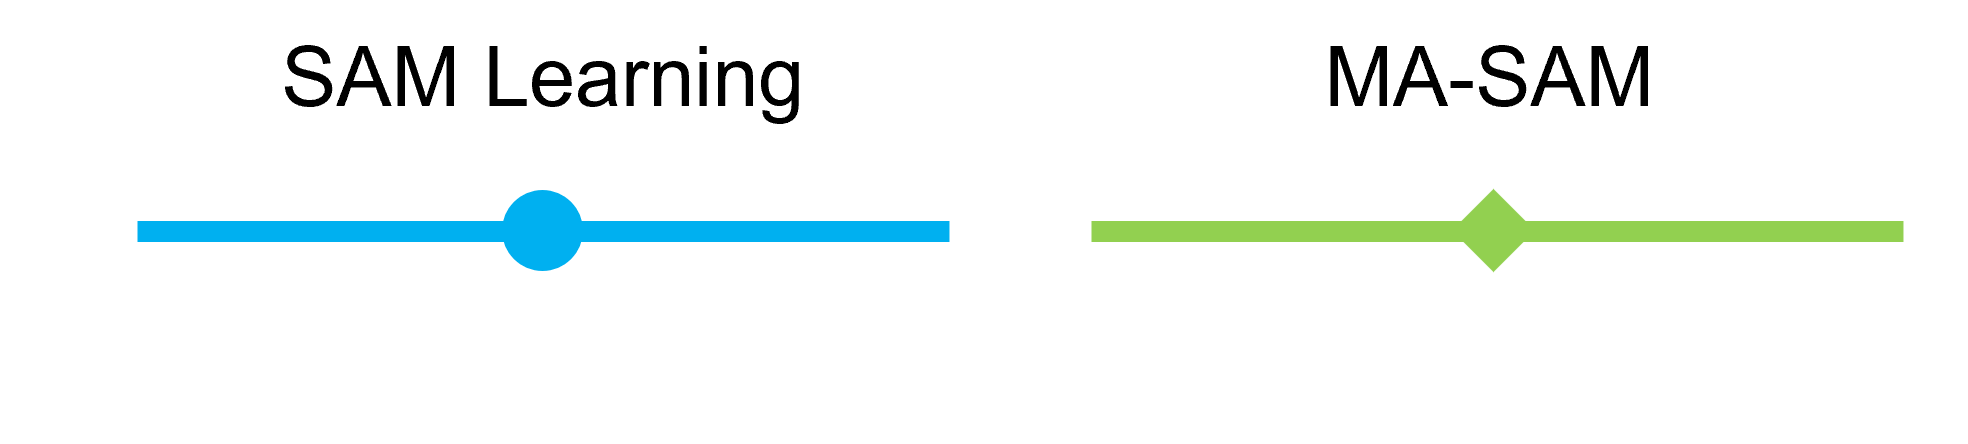
\includegraphics[width=0.8\columnwidth]{figures/legend-graphs.png}
    \label{fig:legend}
  \end{subfigure}
  \begin{subfigure}[b]{\columnwidth}
    \centering
    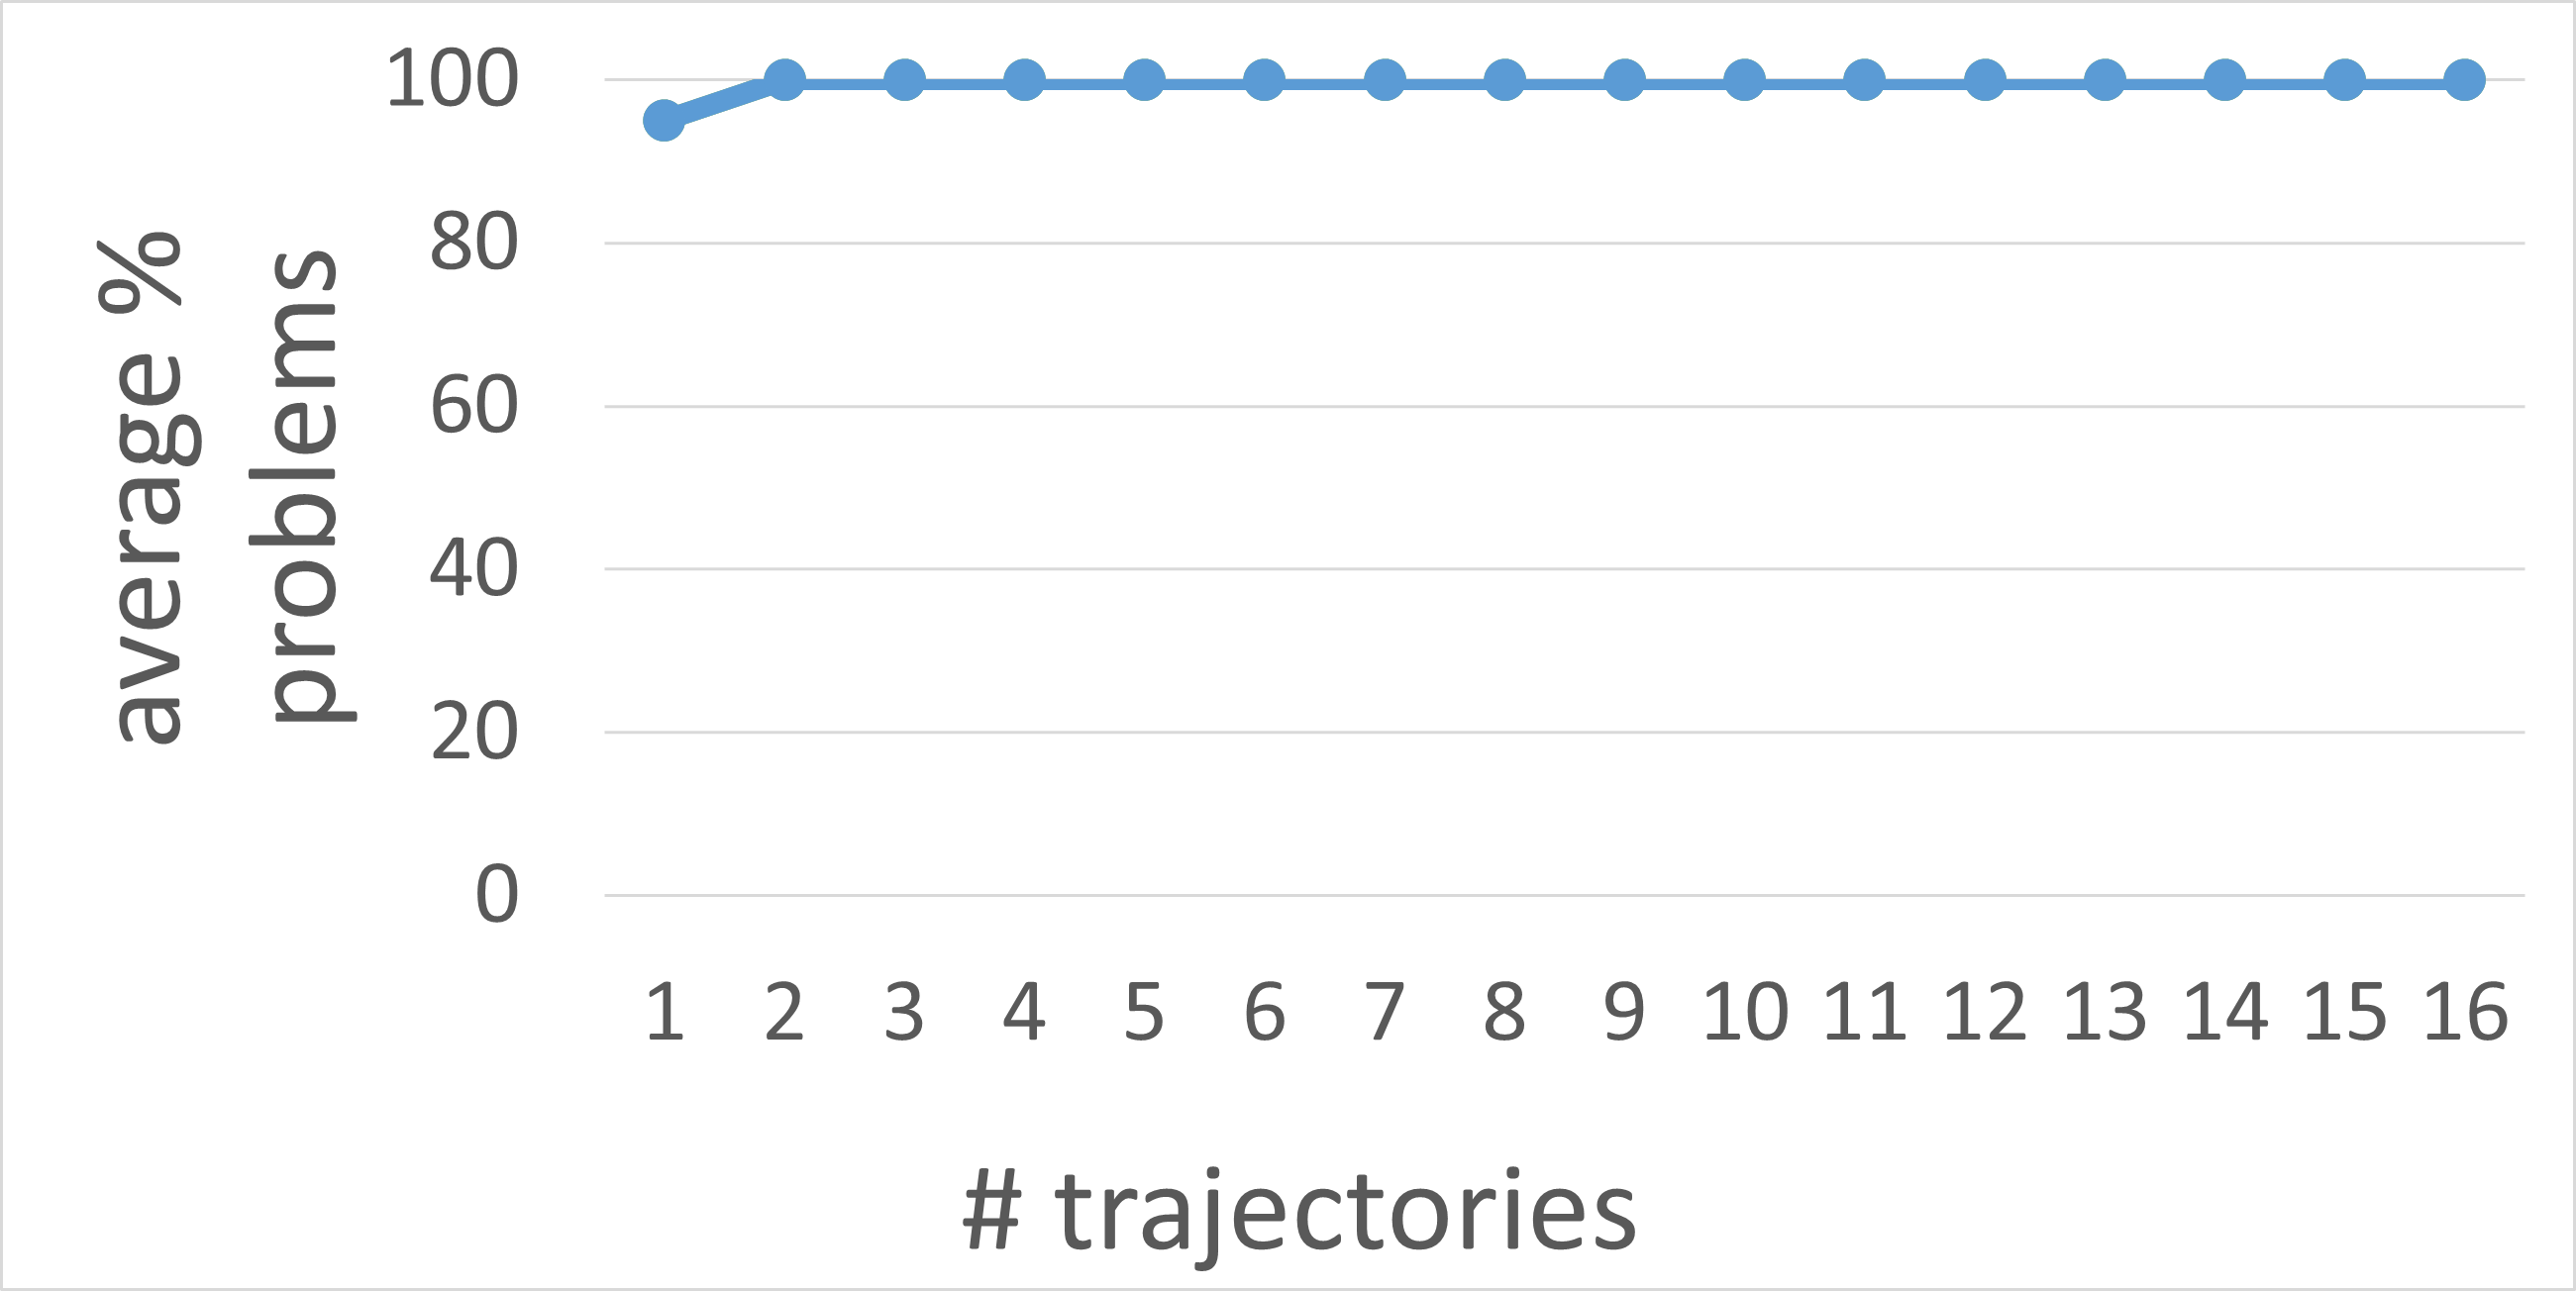
\includegraphics[width=0.48\columnwidth]{figures/sat_easy_learning.png}
    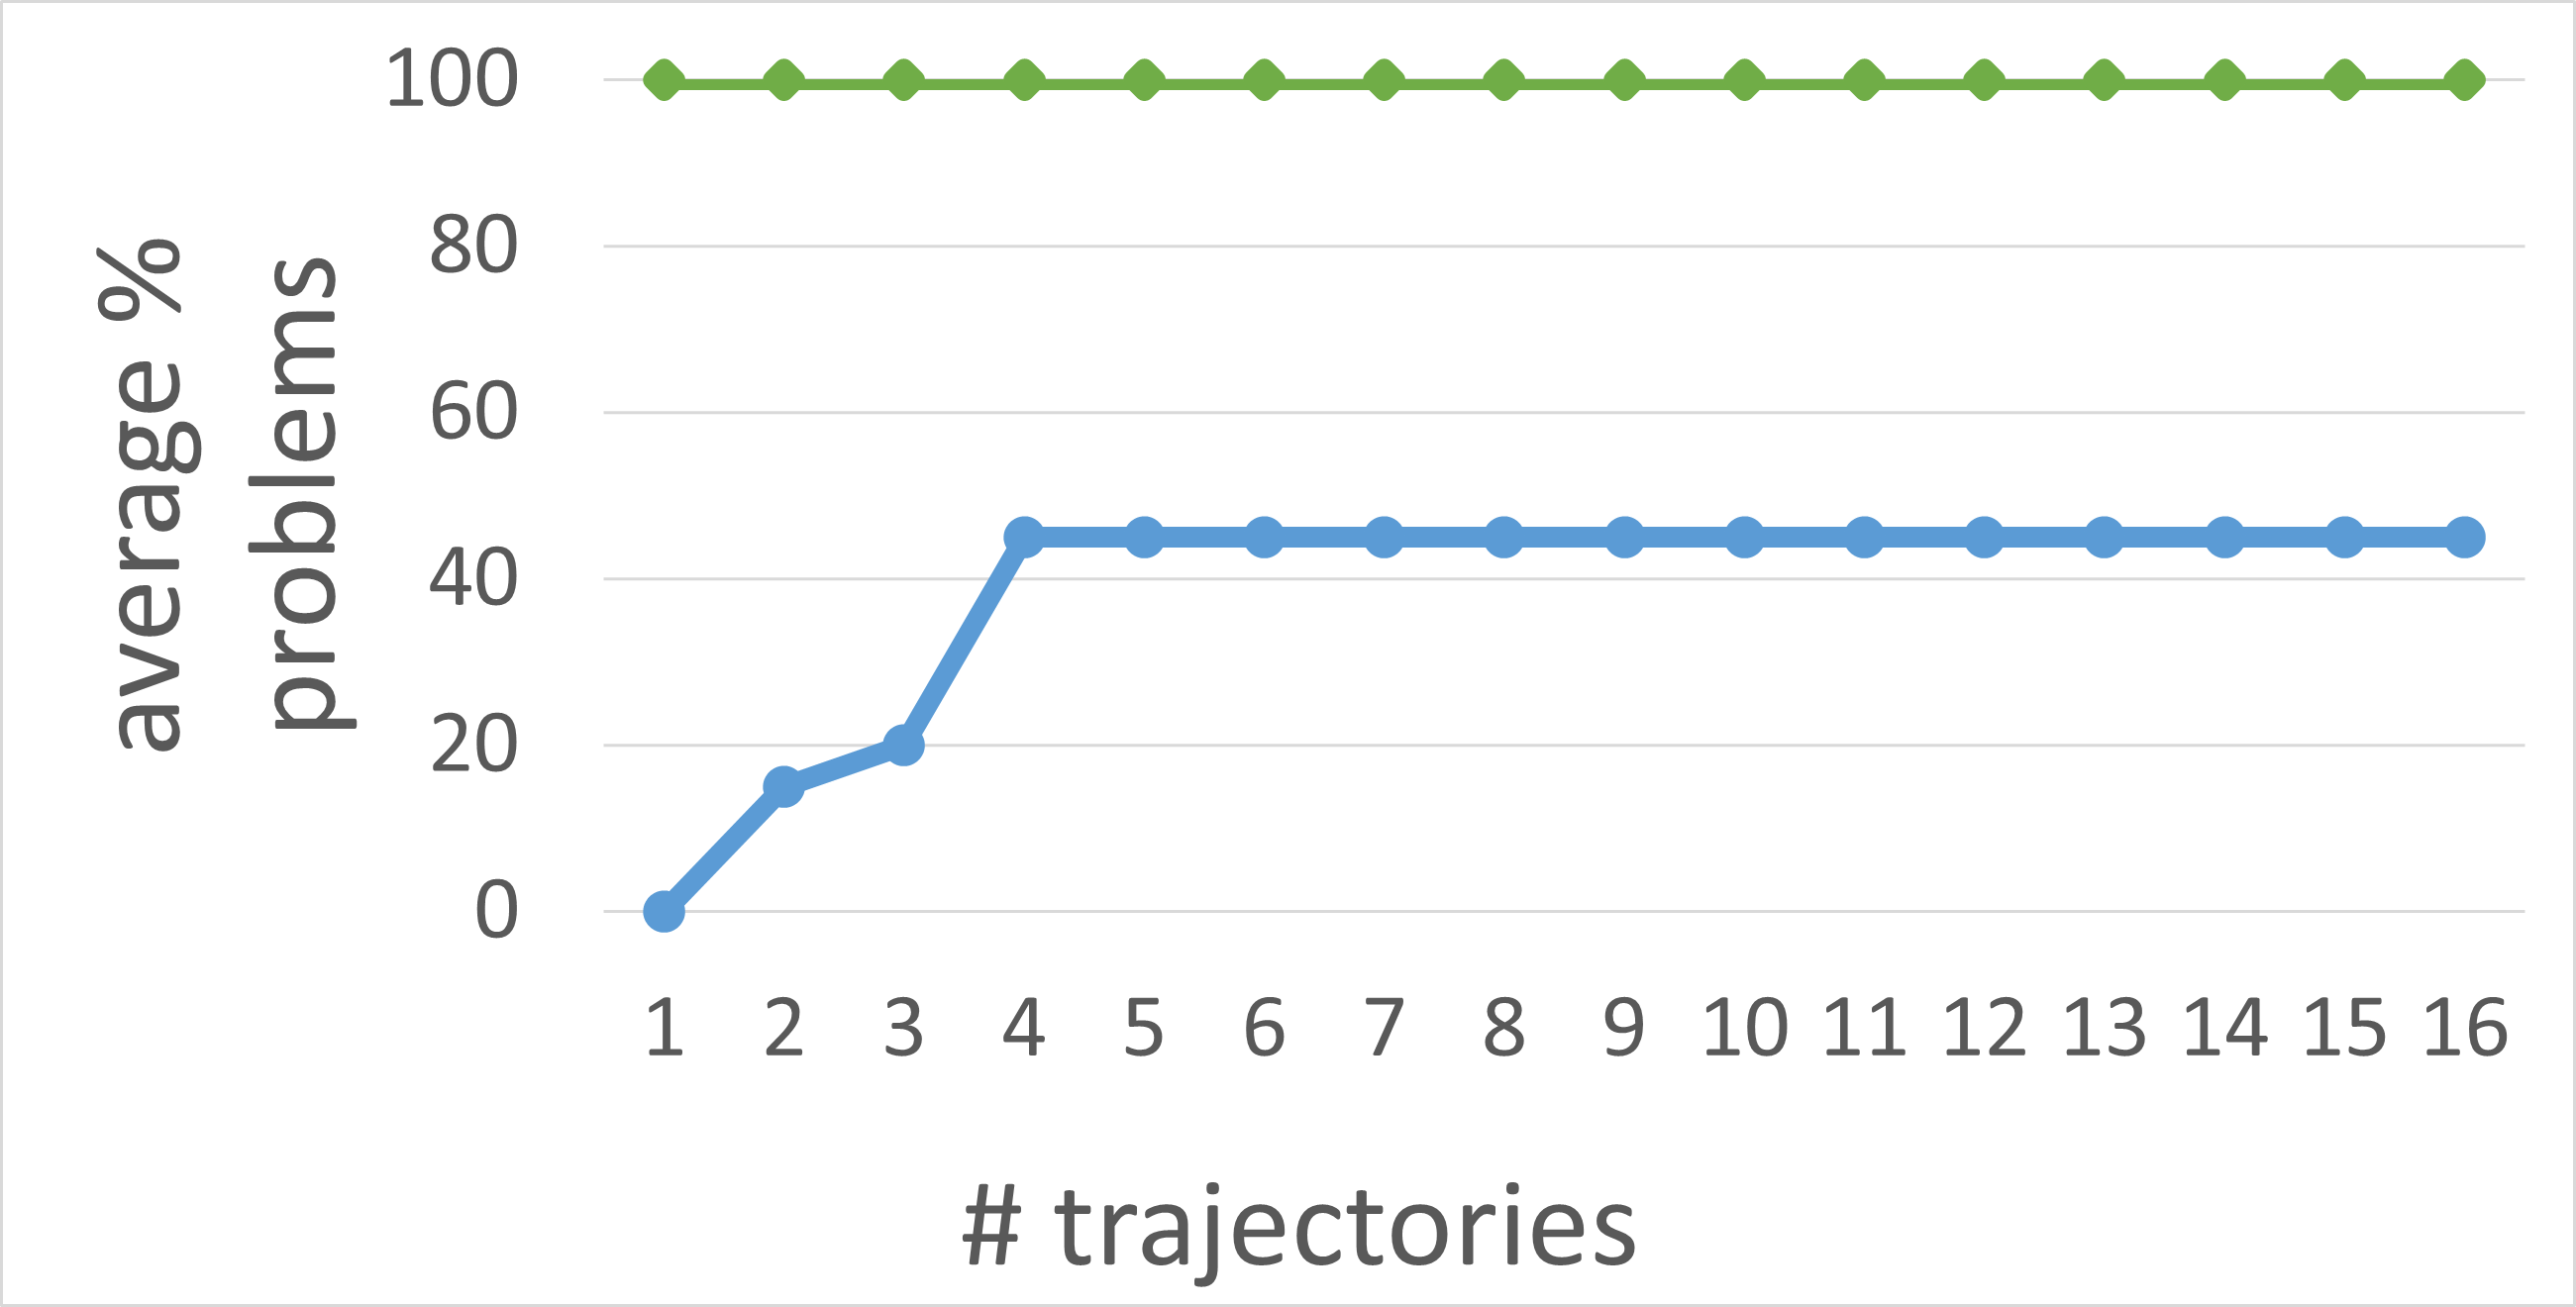
\includegraphics[width=0.48\columnwidth]{figures/sat_hard_learning.png}
    \caption{Satellite}
    \label{fig:sat-results}
  \end{subfigure}
  \begin{subfigure}[b]{\columnwidth}
    \centering
    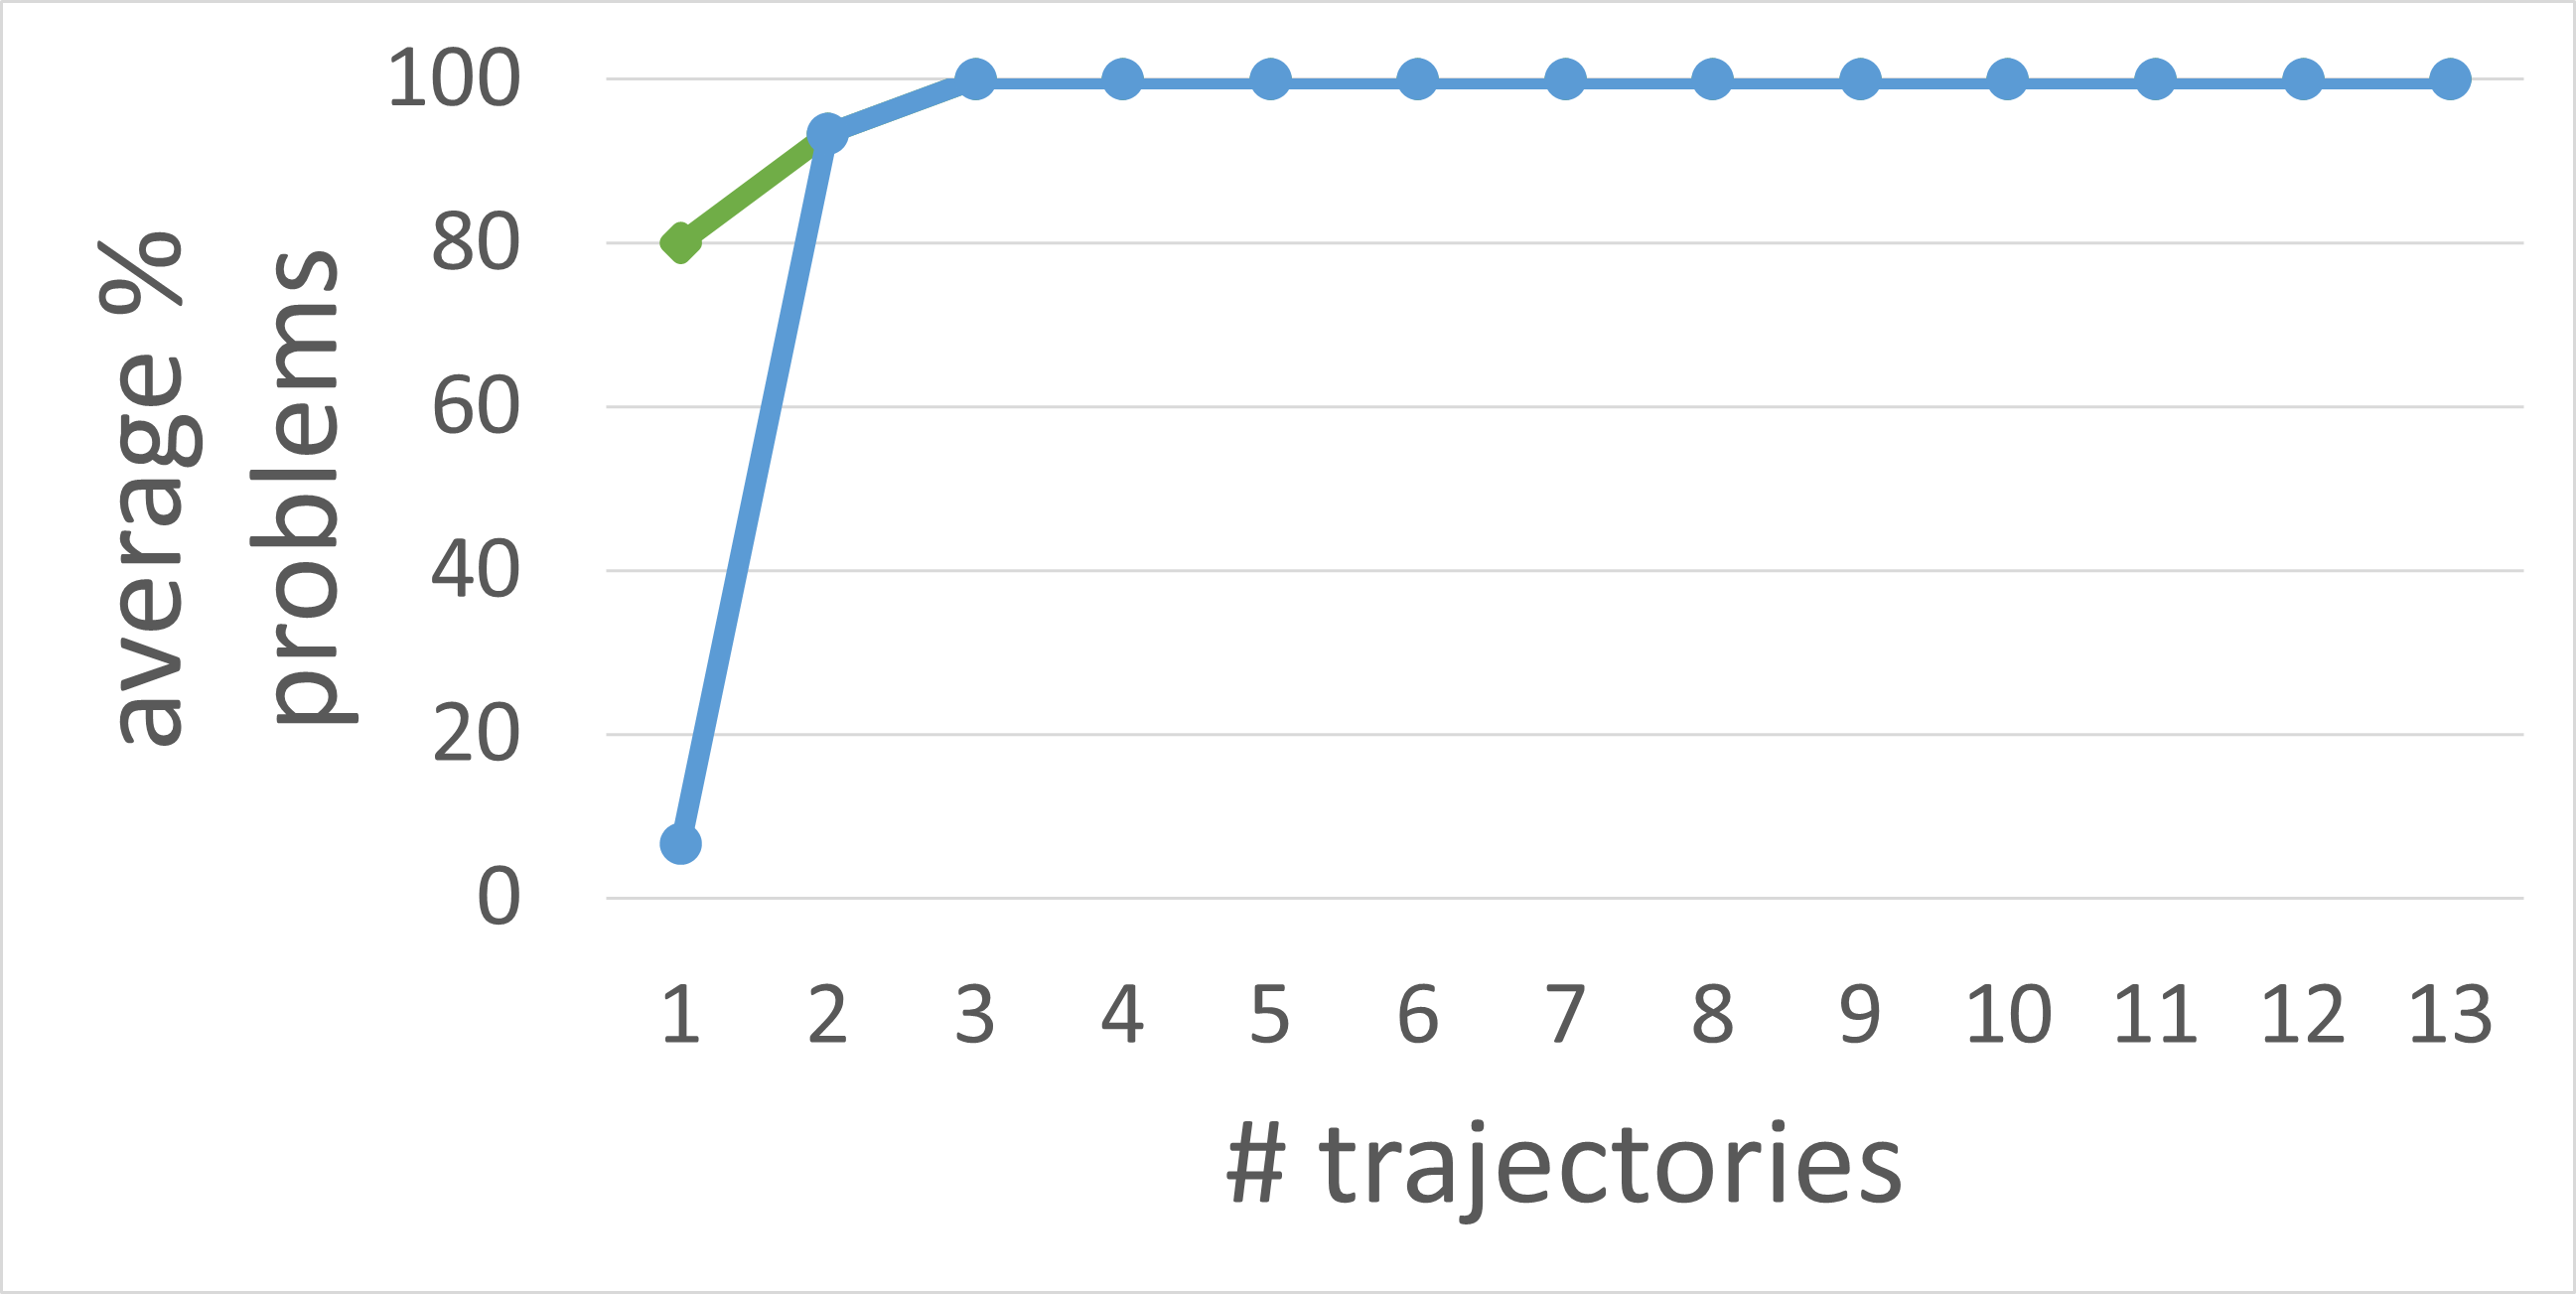
\includegraphics[width=0.48\columnwidth]{figures/driverlog_easy_learning.png}
    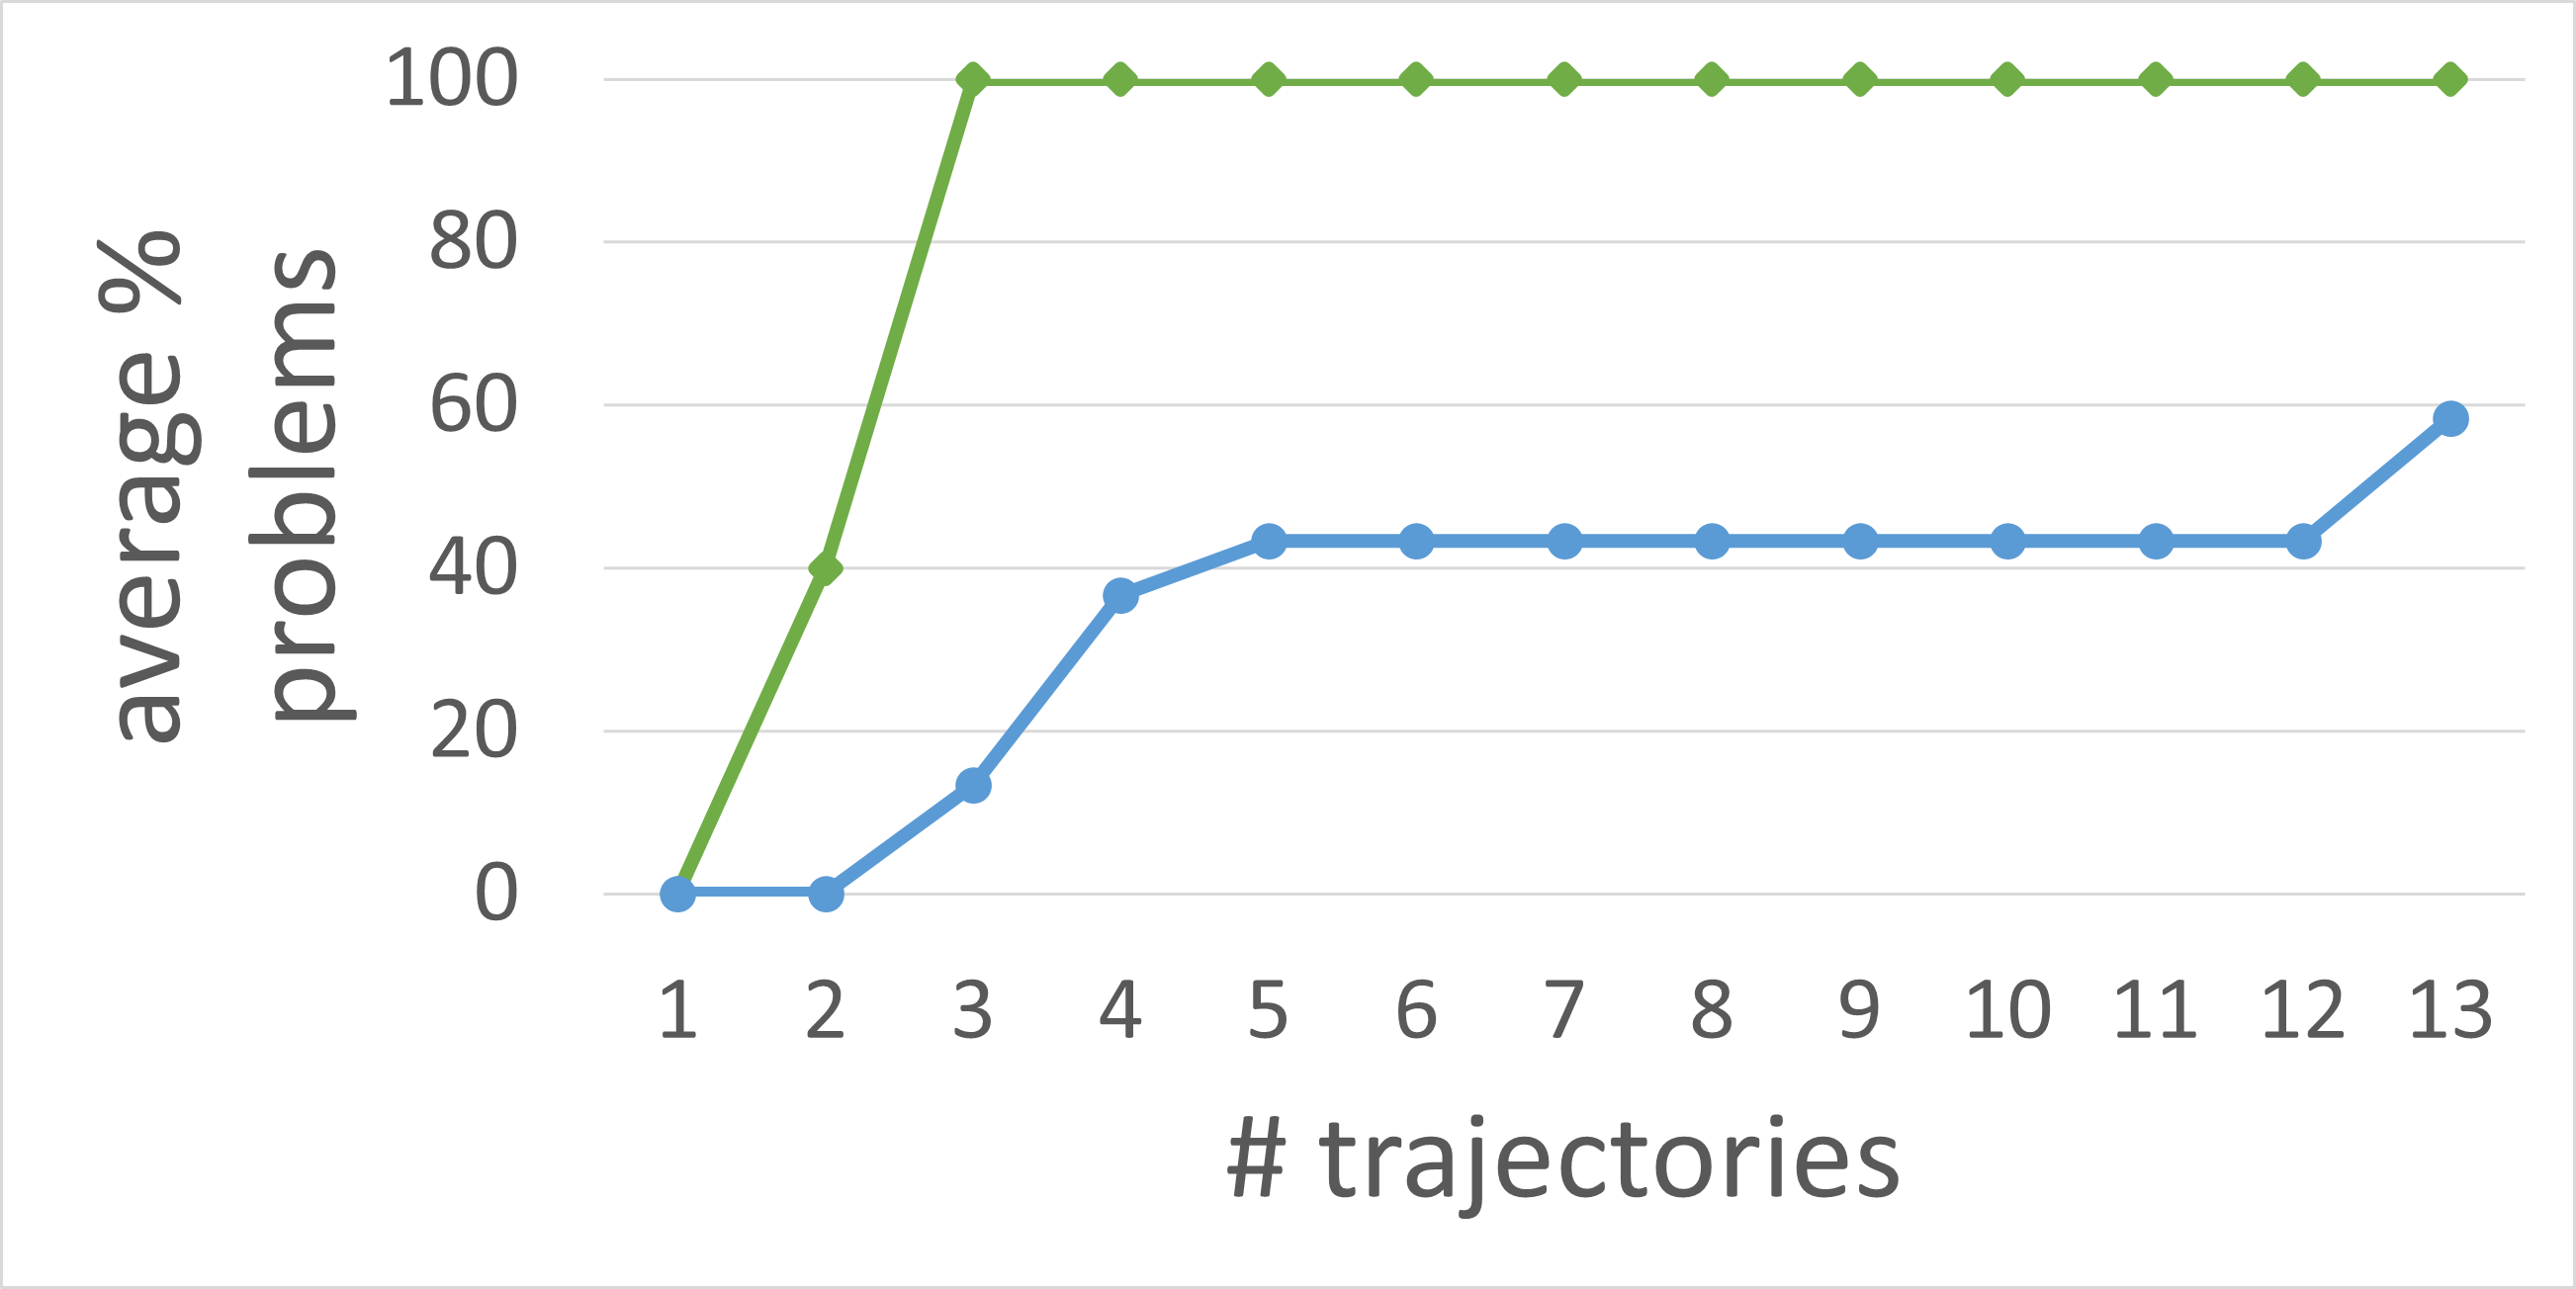
\includegraphics[width=0.48\columnwidth]{figures/driverlog_hard_learning.png}
    \caption{Driverlog}
    \label{fig:driverlog-results}
  \end{subfigure}\\
  \begin{subfigure}[b]{\columnwidth}
    \centering
    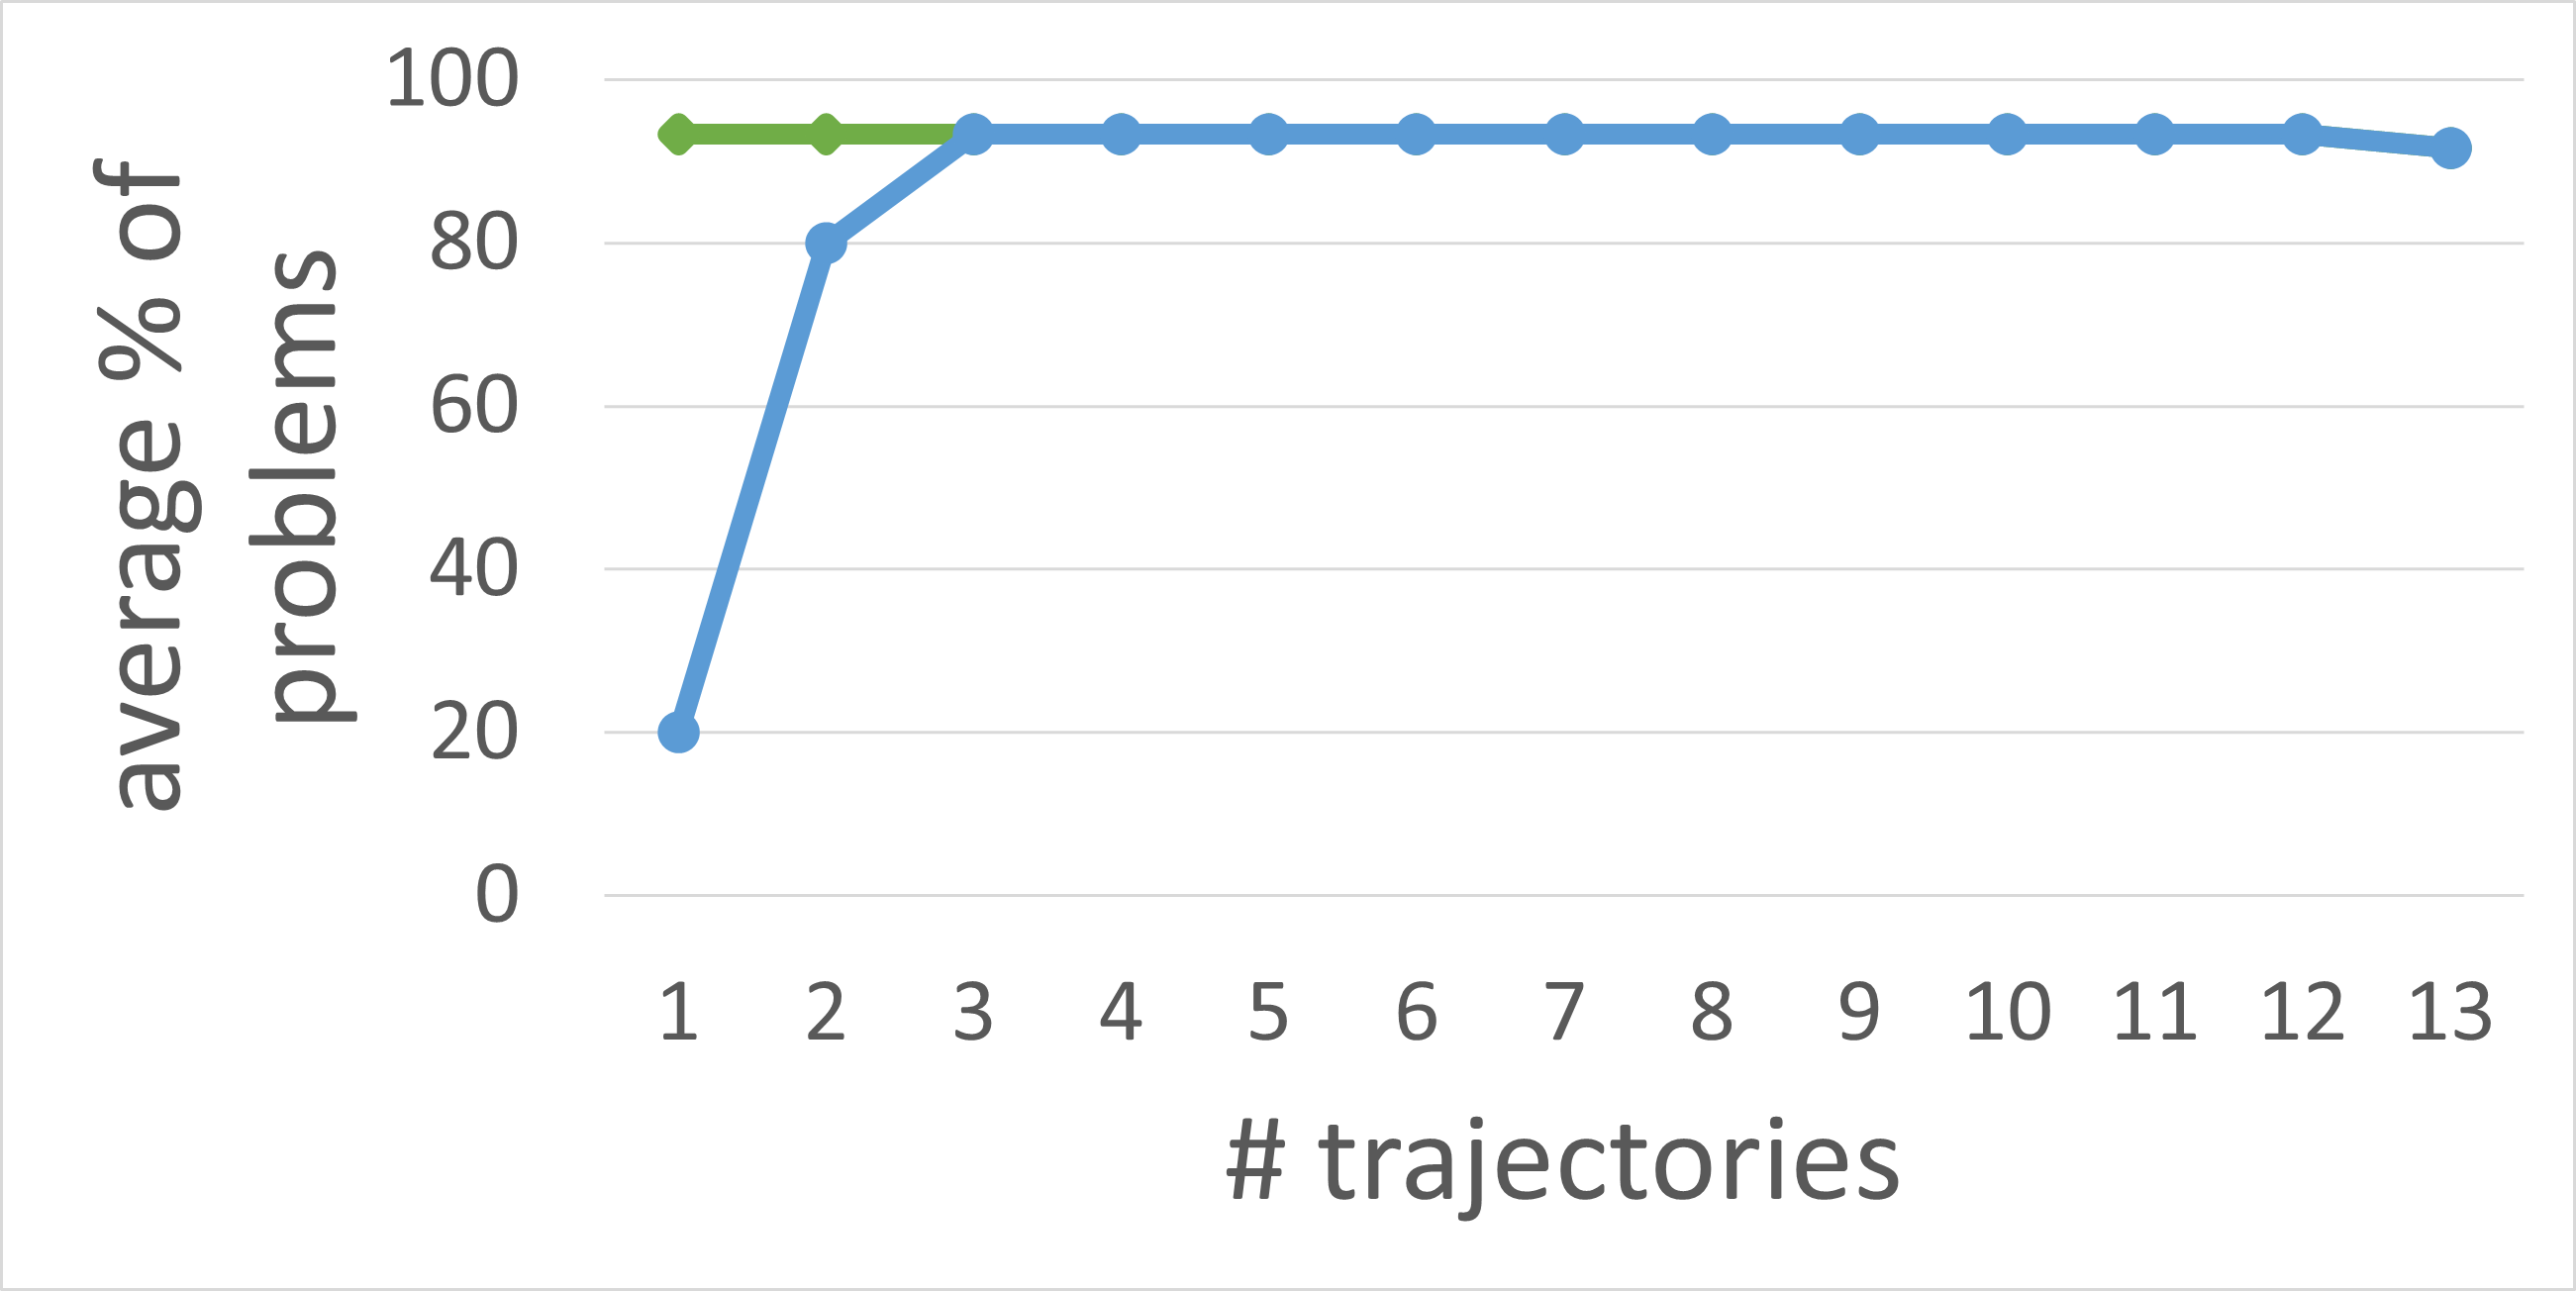
\includegraphics[width=0.48\columnwidth]{figures/depot_easy_learning.png}
    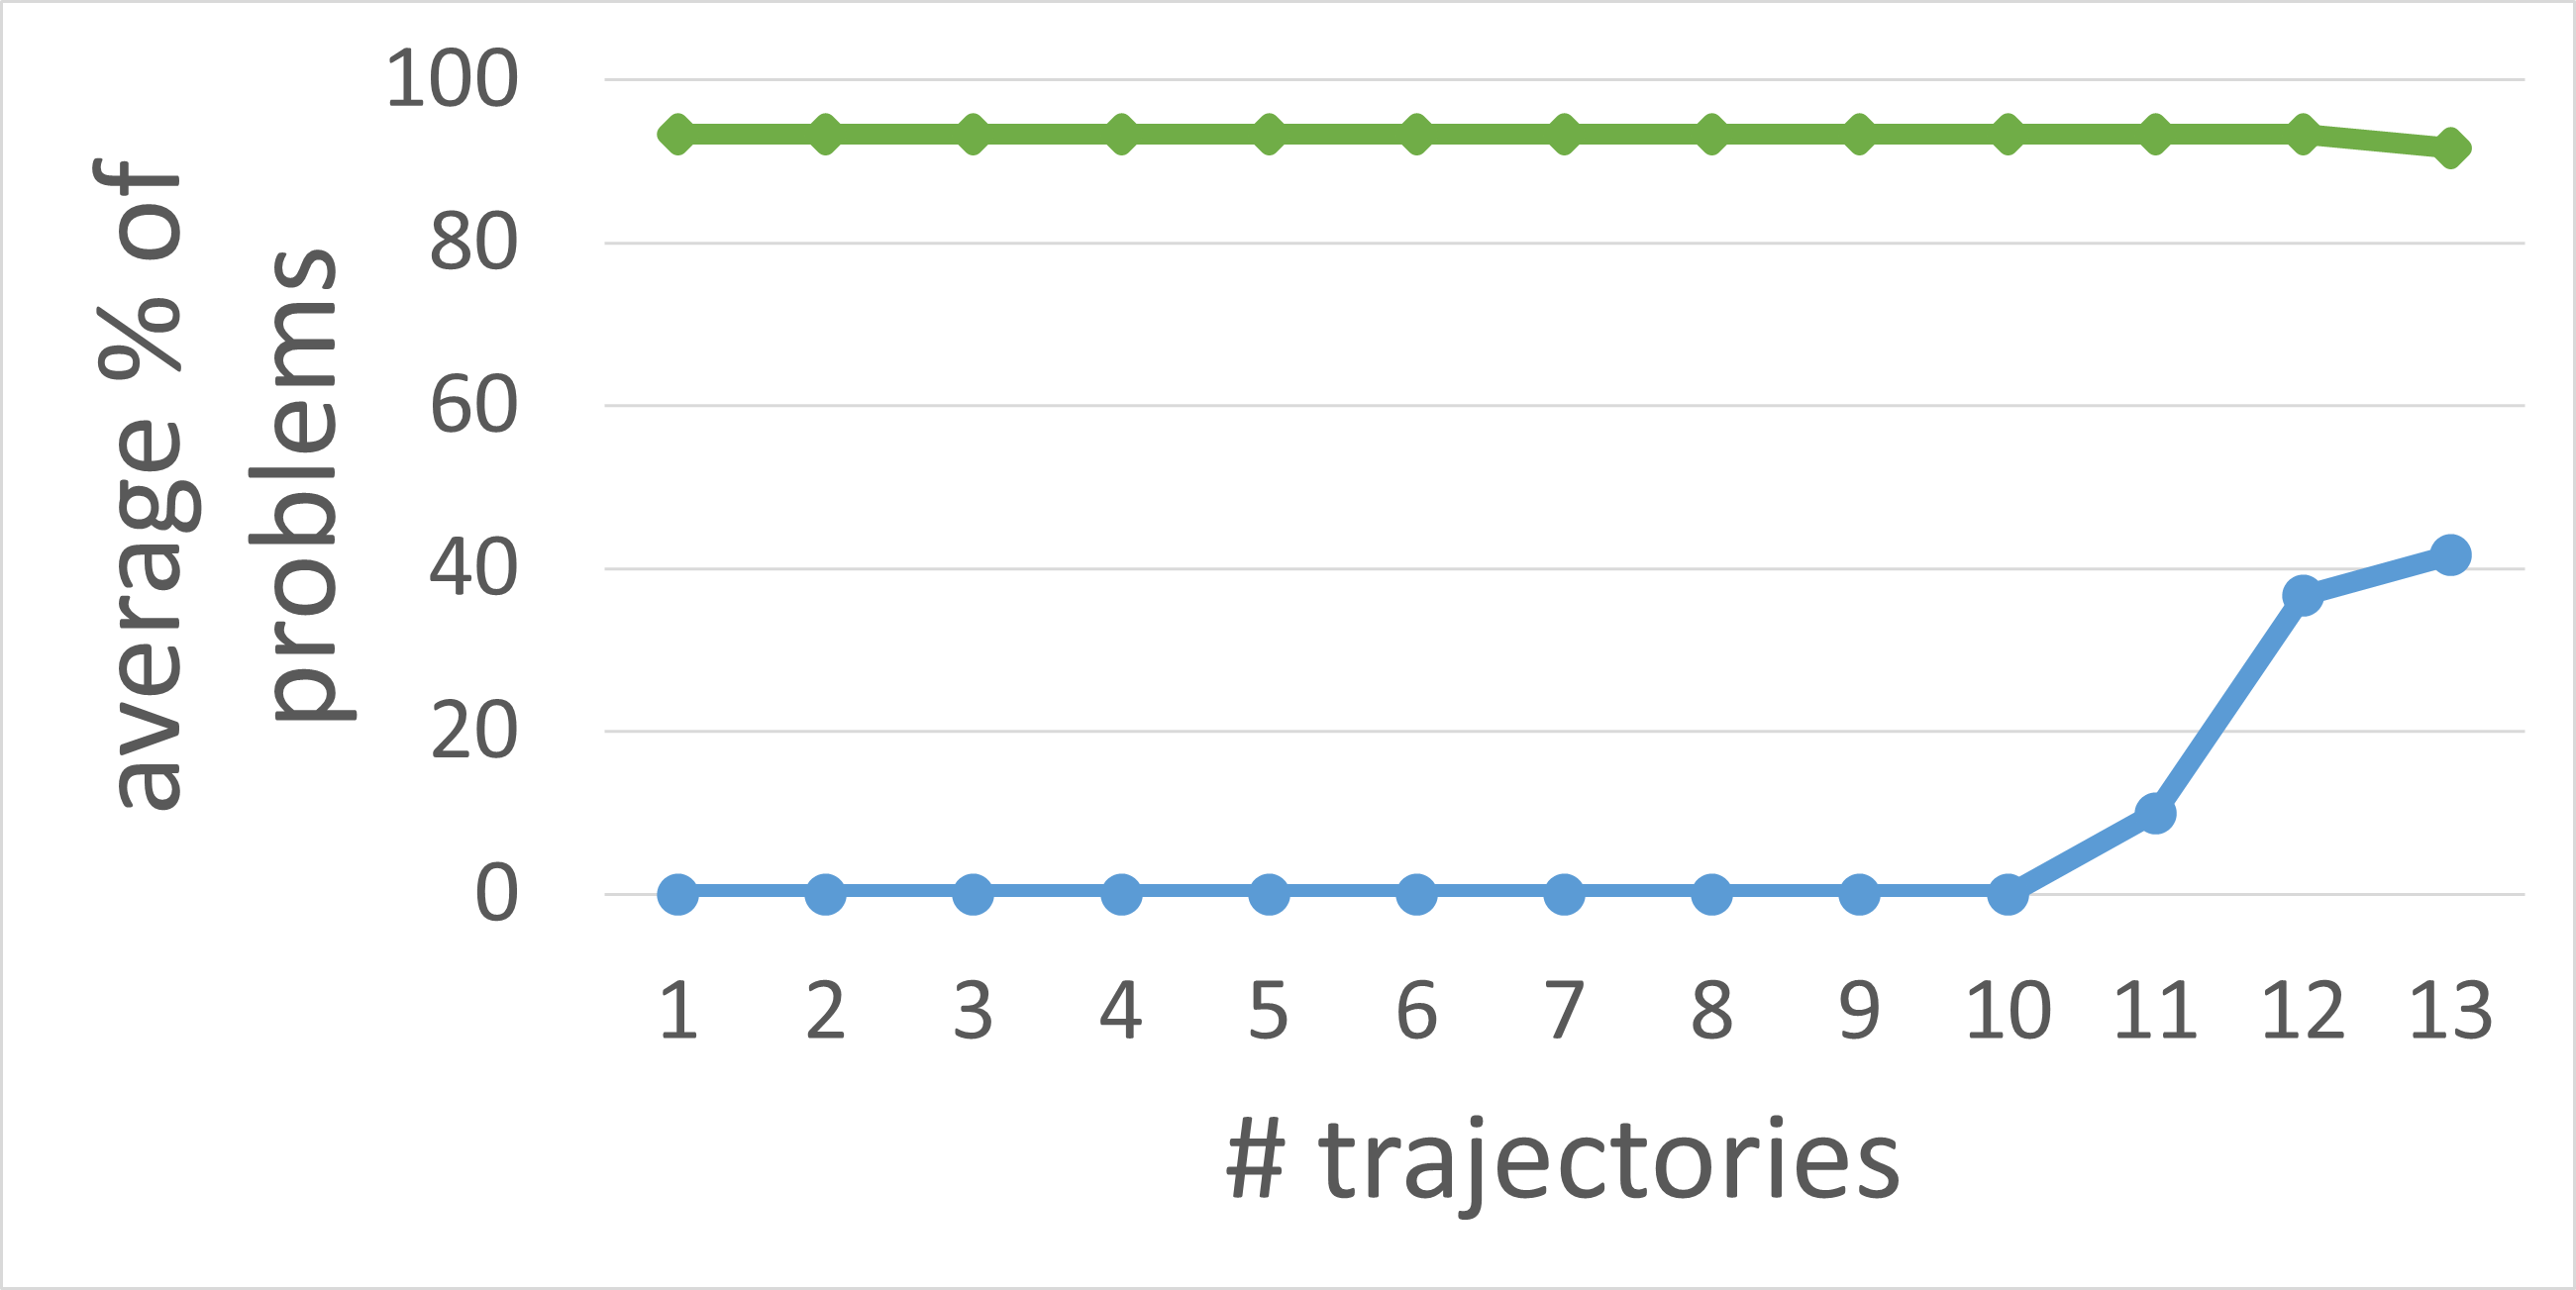
\includegraphics[width=0.48\columnwidth]{figures/depot_hard_learning.png}
    \caption{Depots}
    \label{fig:depots-results}
  \end{subfigure}
  \begin{subfigure}[b]{\columnwidth}
    \centering
    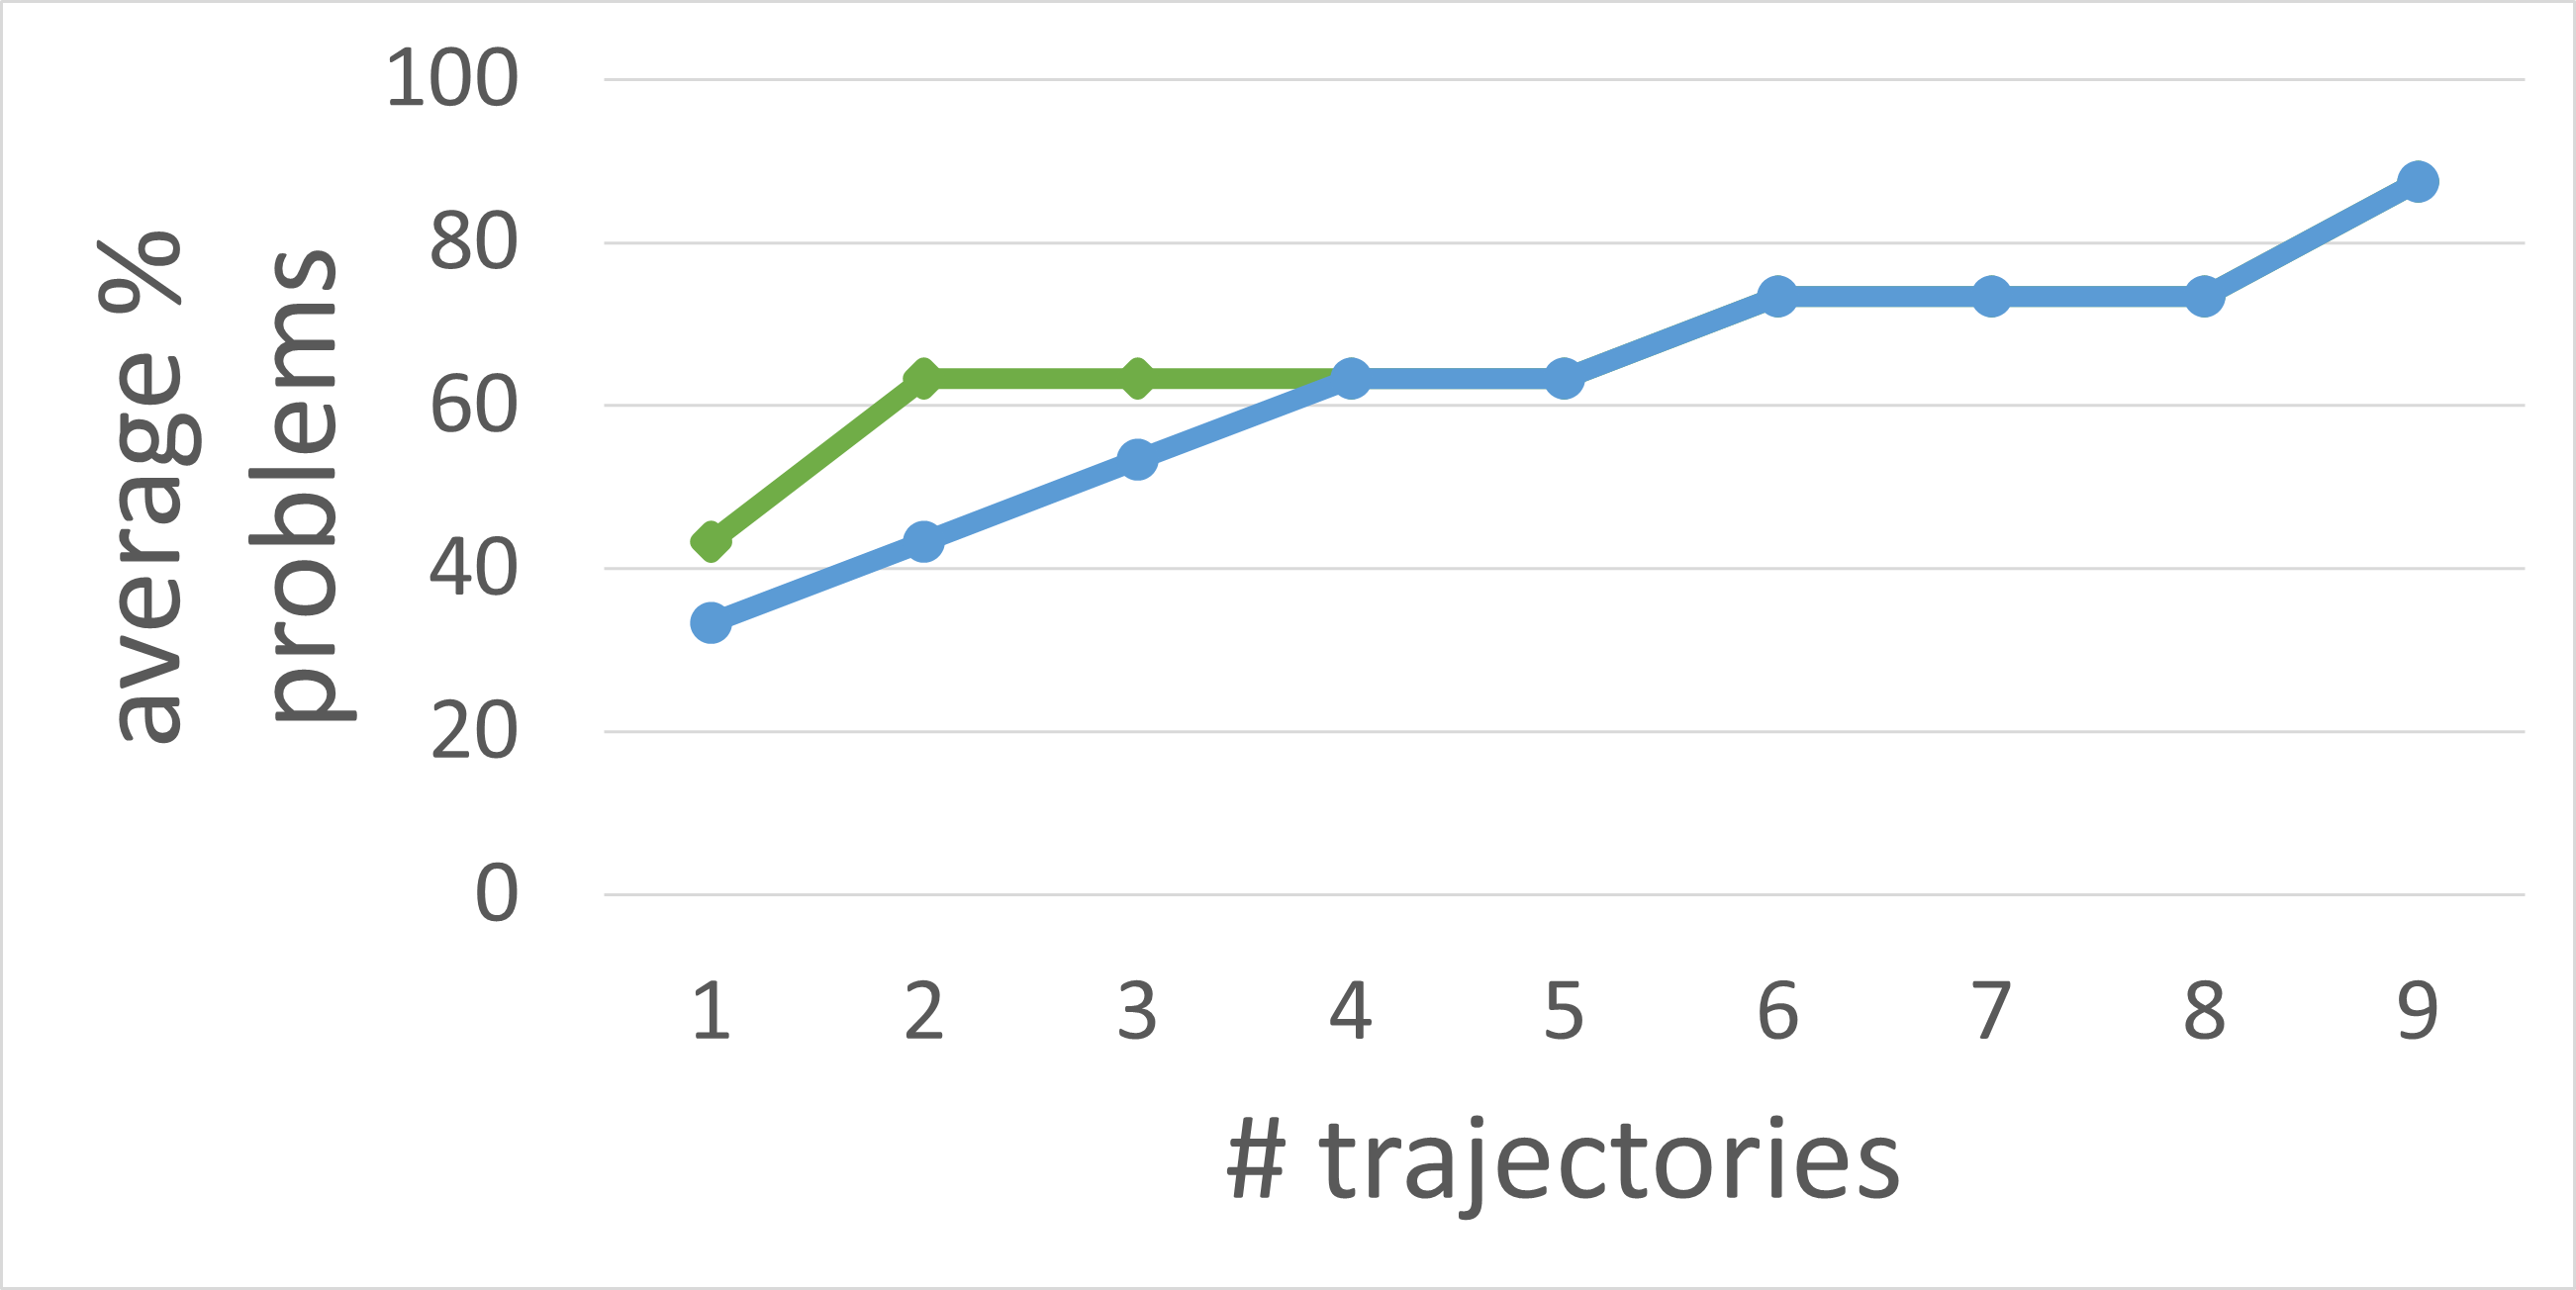
\includegraphics[width=0.48\columnwidth]{figures/sok_easy_learning.png}
    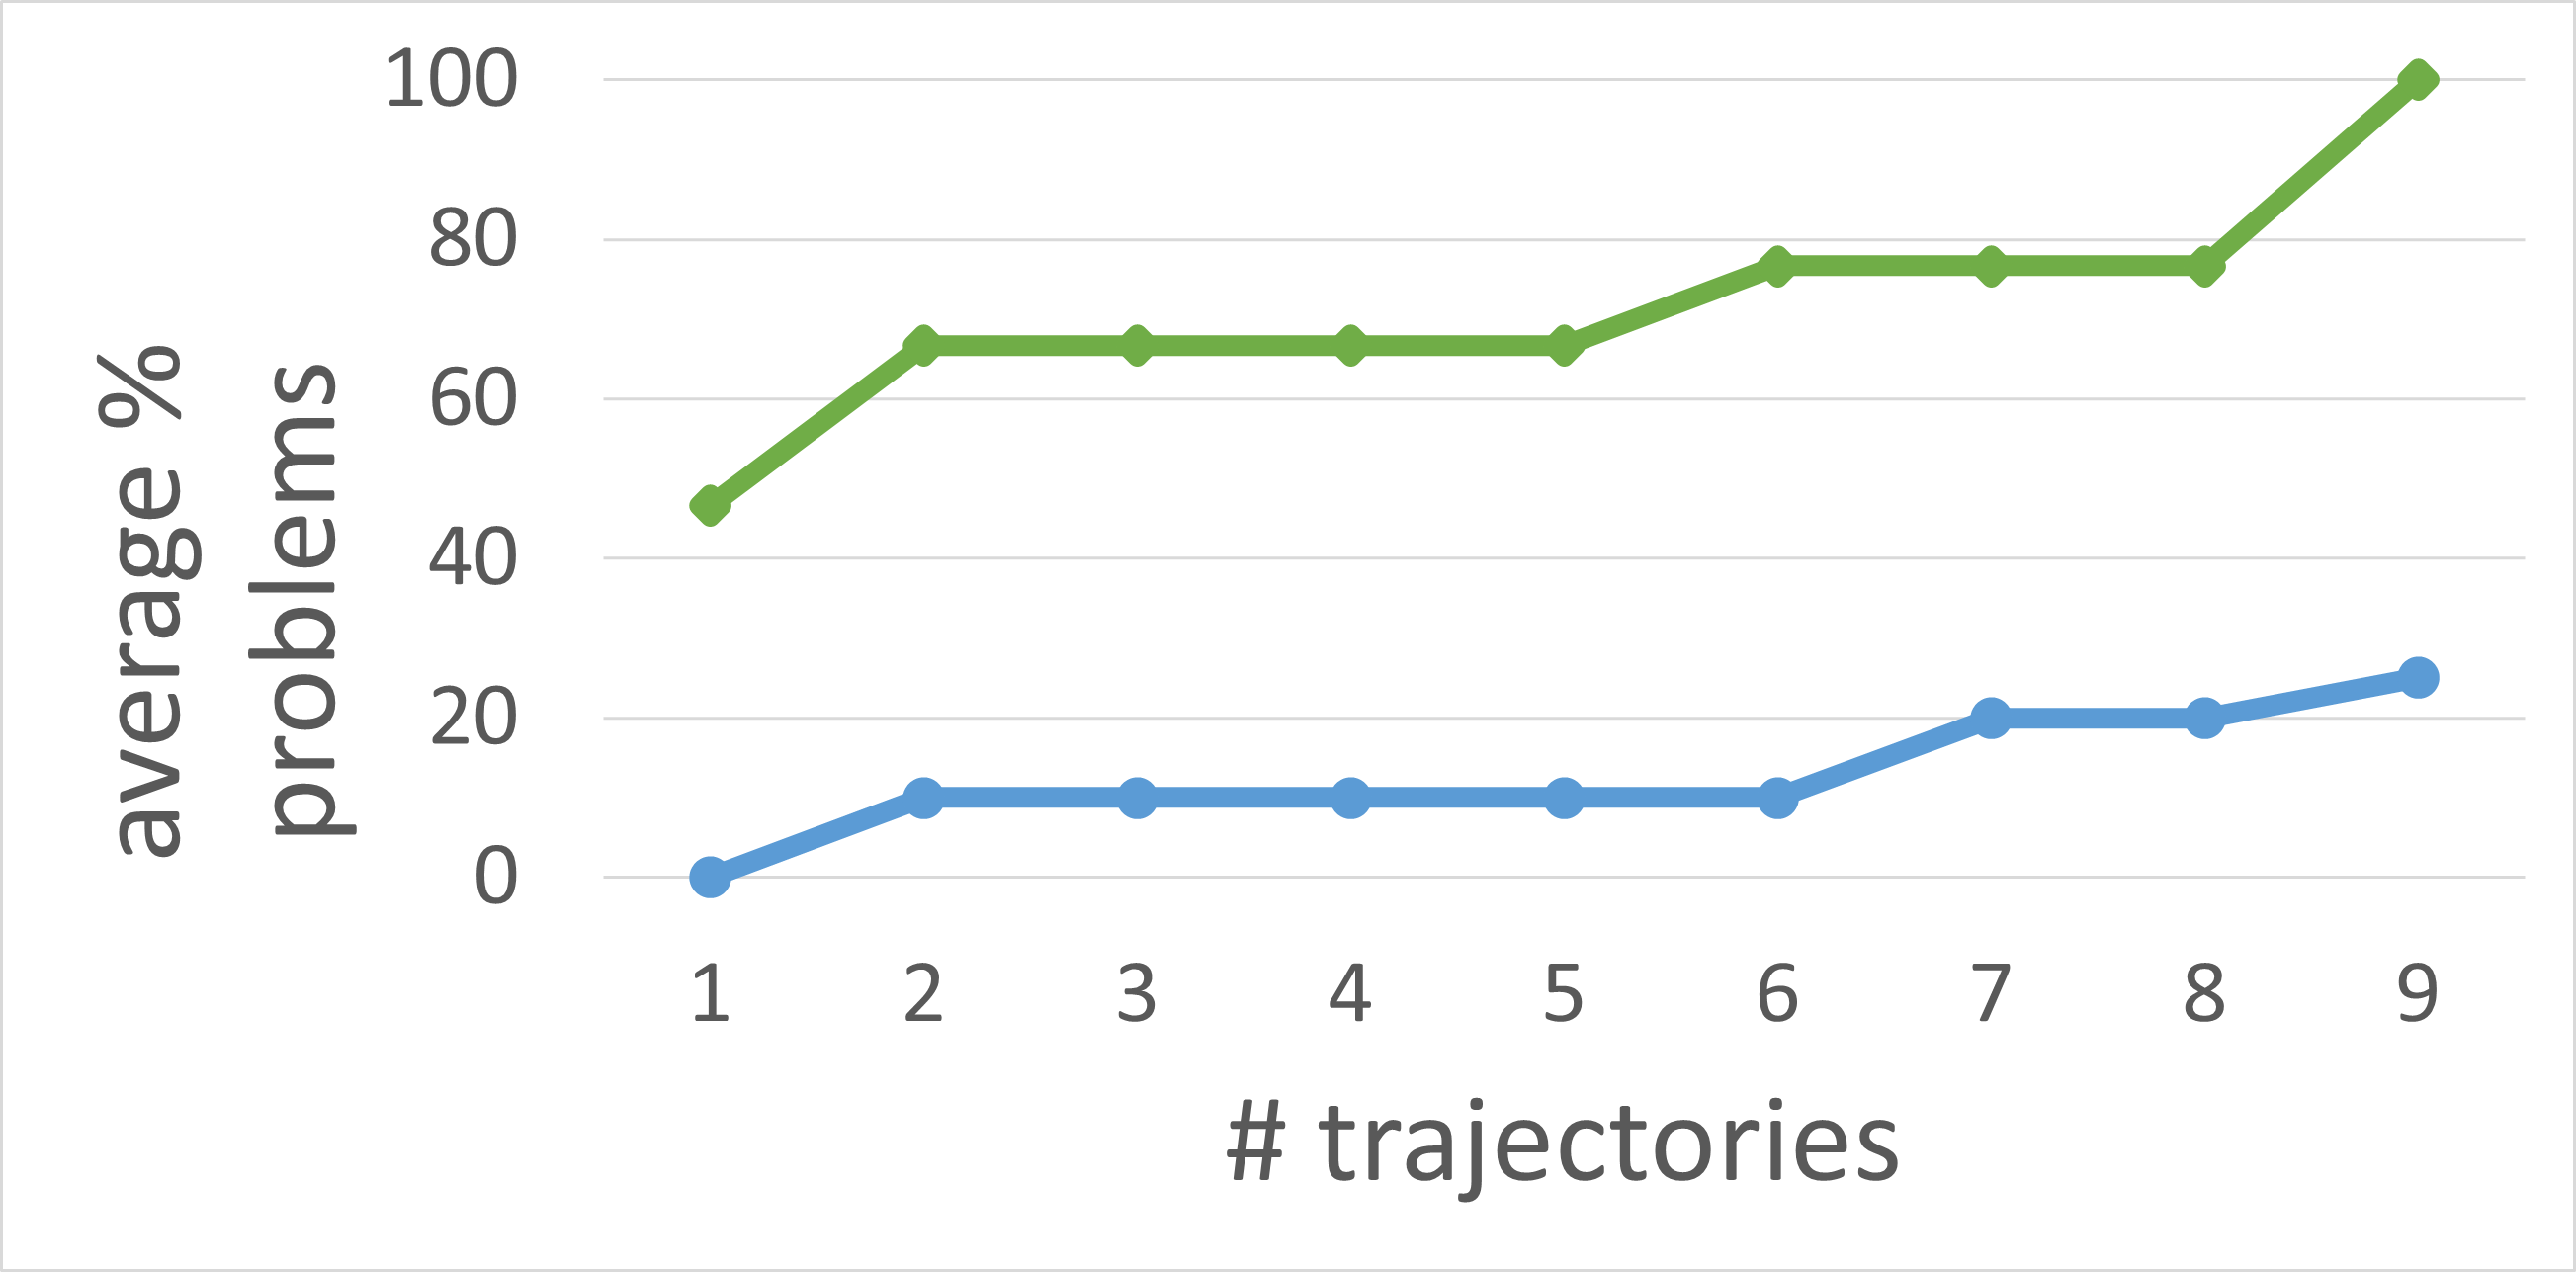
\includegraphics[width=0.48\columnwidth]{figures/sok_hard_learning.png}
    \caption{Sokoban}
    \label{fig:sokoban-results}
  \end{subfigure}\\
  \begin{subfigure}[b]{\columnwidth}
    \centering
    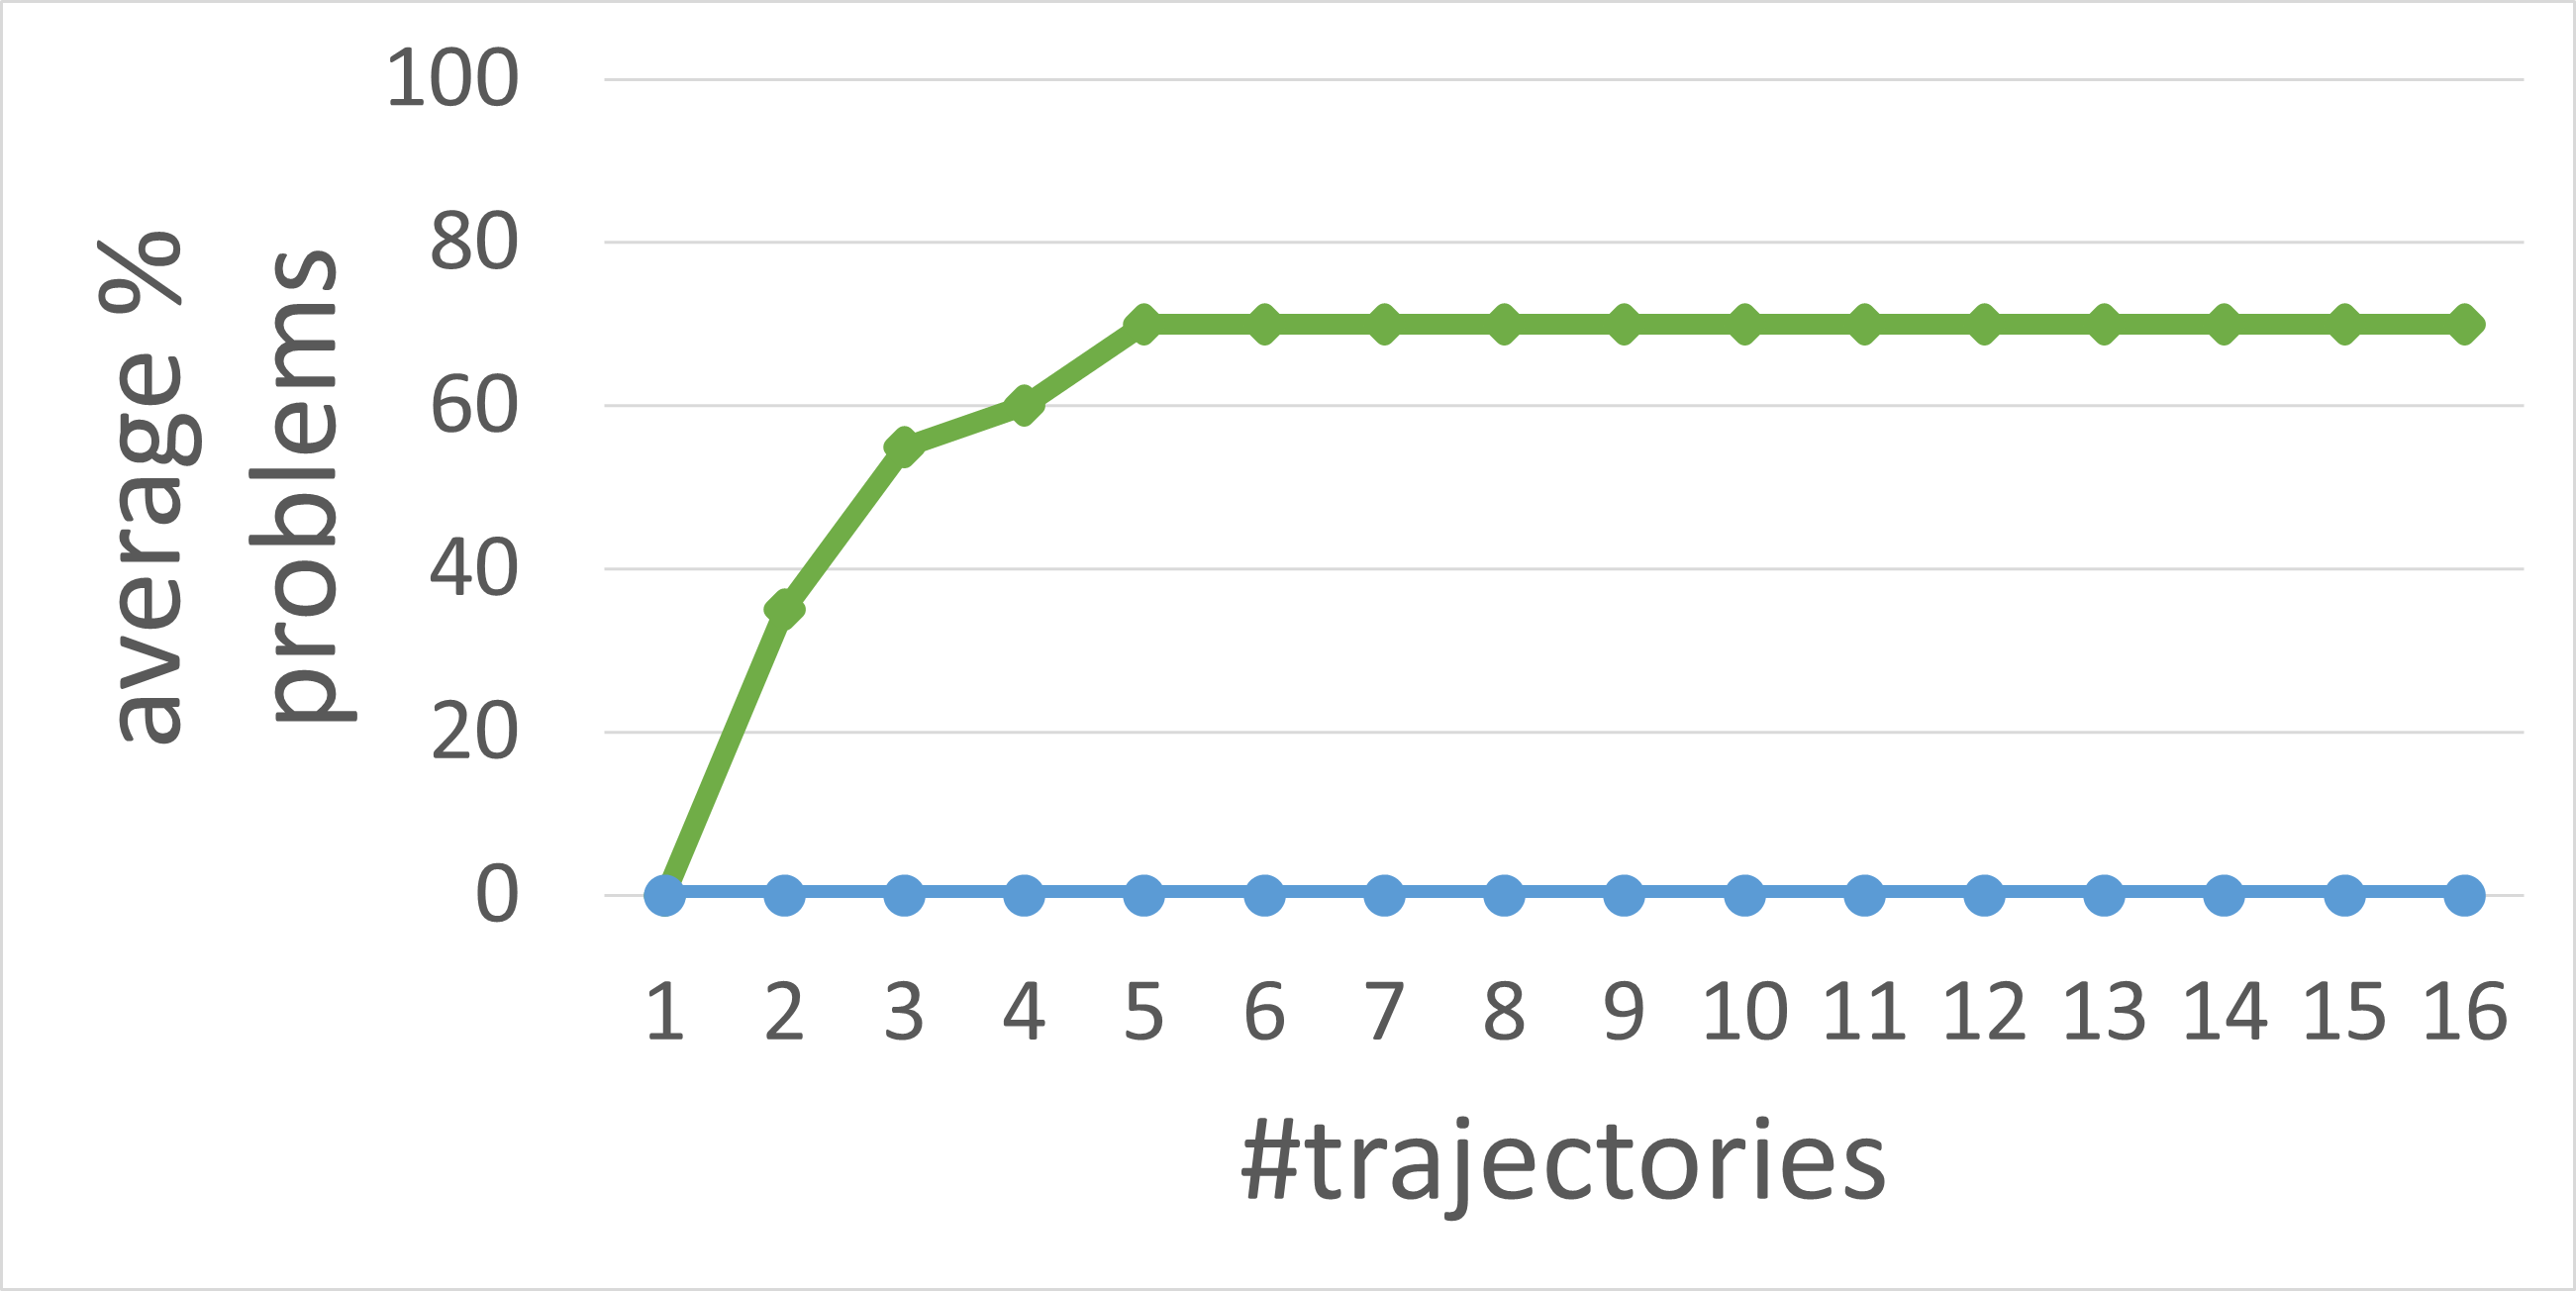
\includegraphics[width=0.48\columnwidth]{figures/rover_easy_learning.png}
    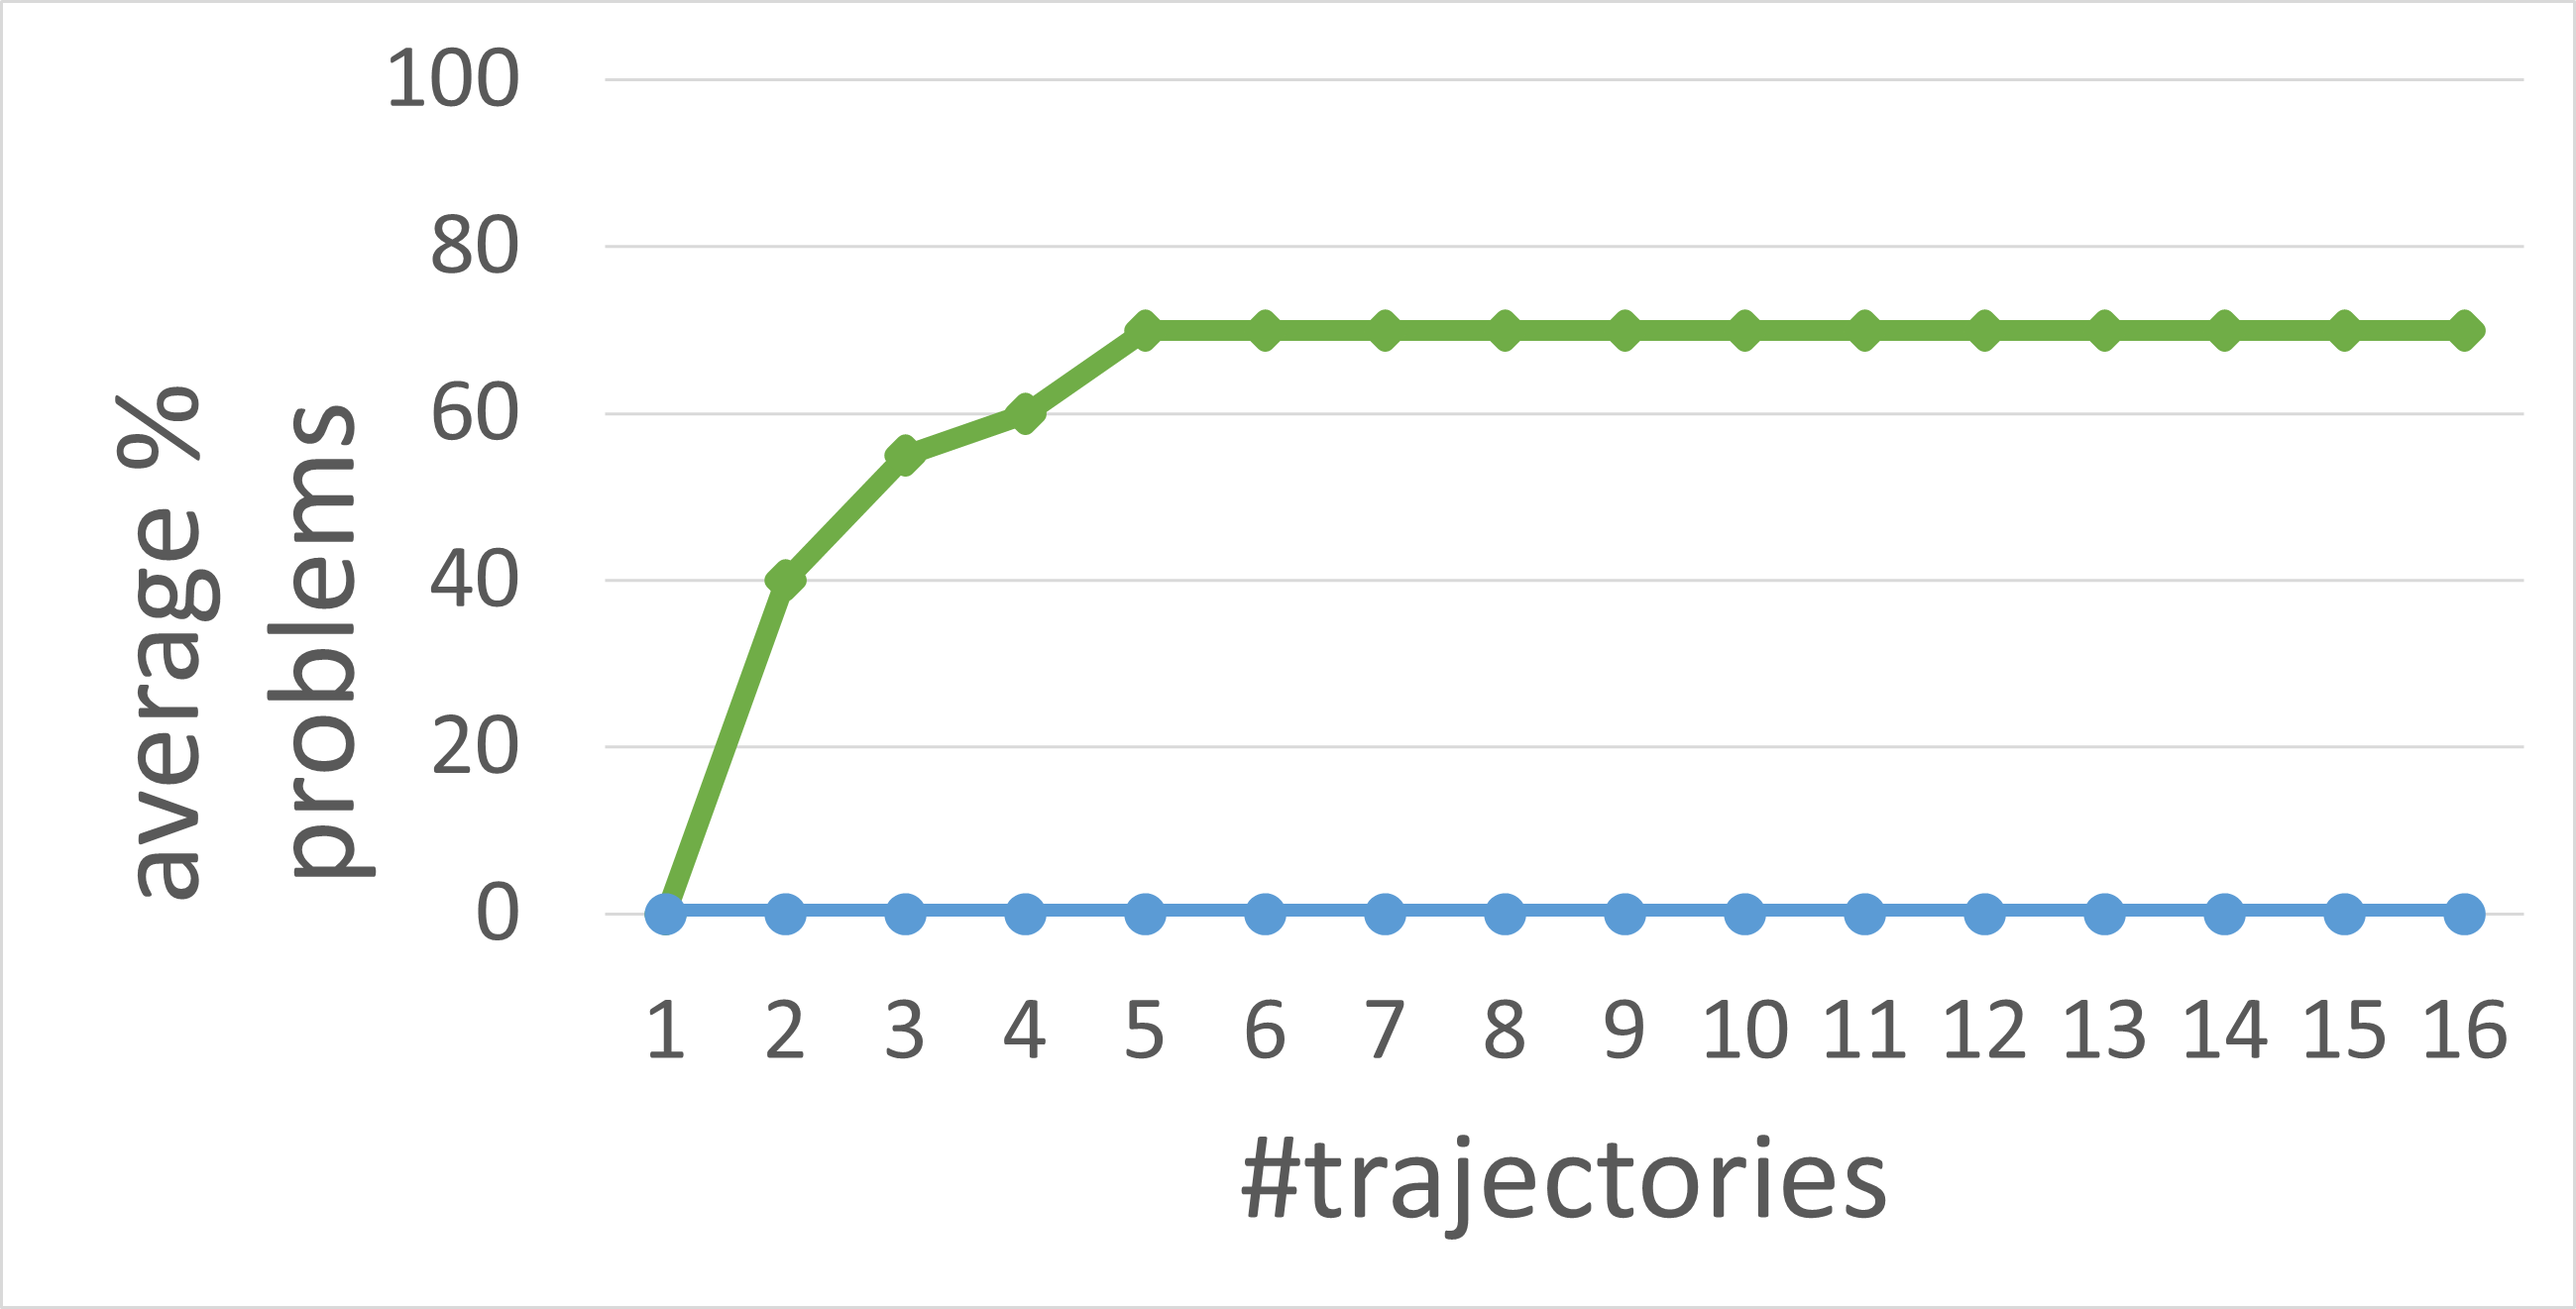
\includegraphics[width=0.48\columnwidth]{figures/rover_hard_learning.png}
    \caption{Rovers}
    \label{fig:rovers-results}
  \end{subfigure}
  \begin{subfigure}[b]{\columnwidth}
    \centering
    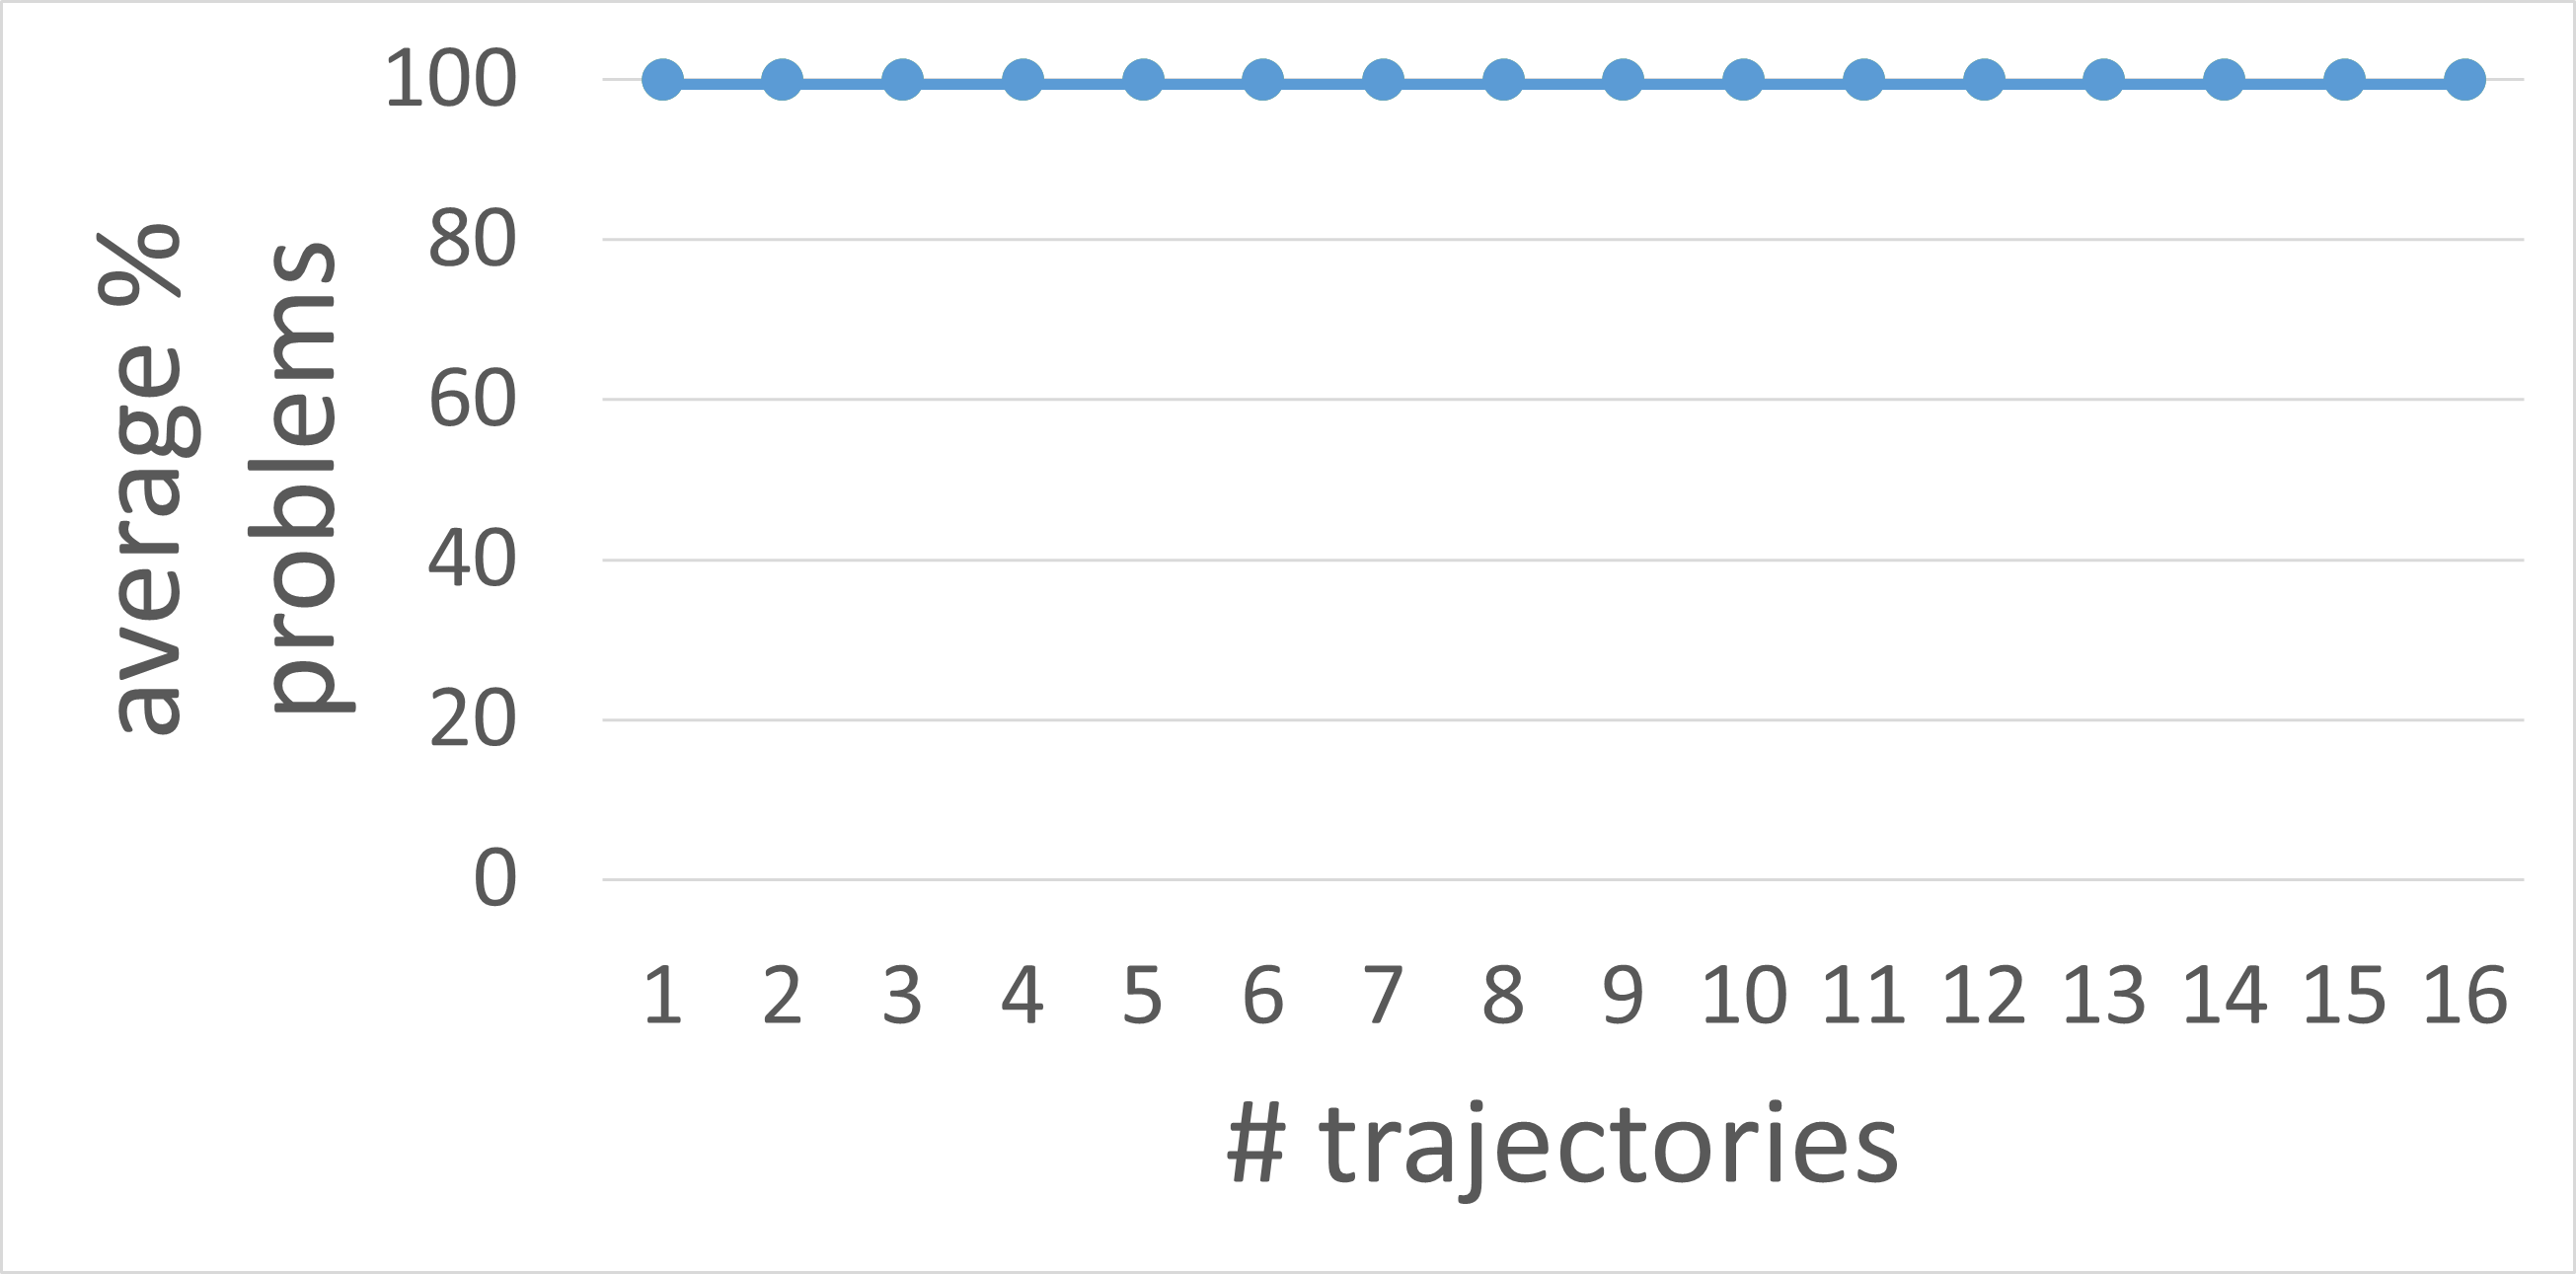
\includegraphics[width=0.48\columnwidth]{figures/logistics_easy_learning.png}
    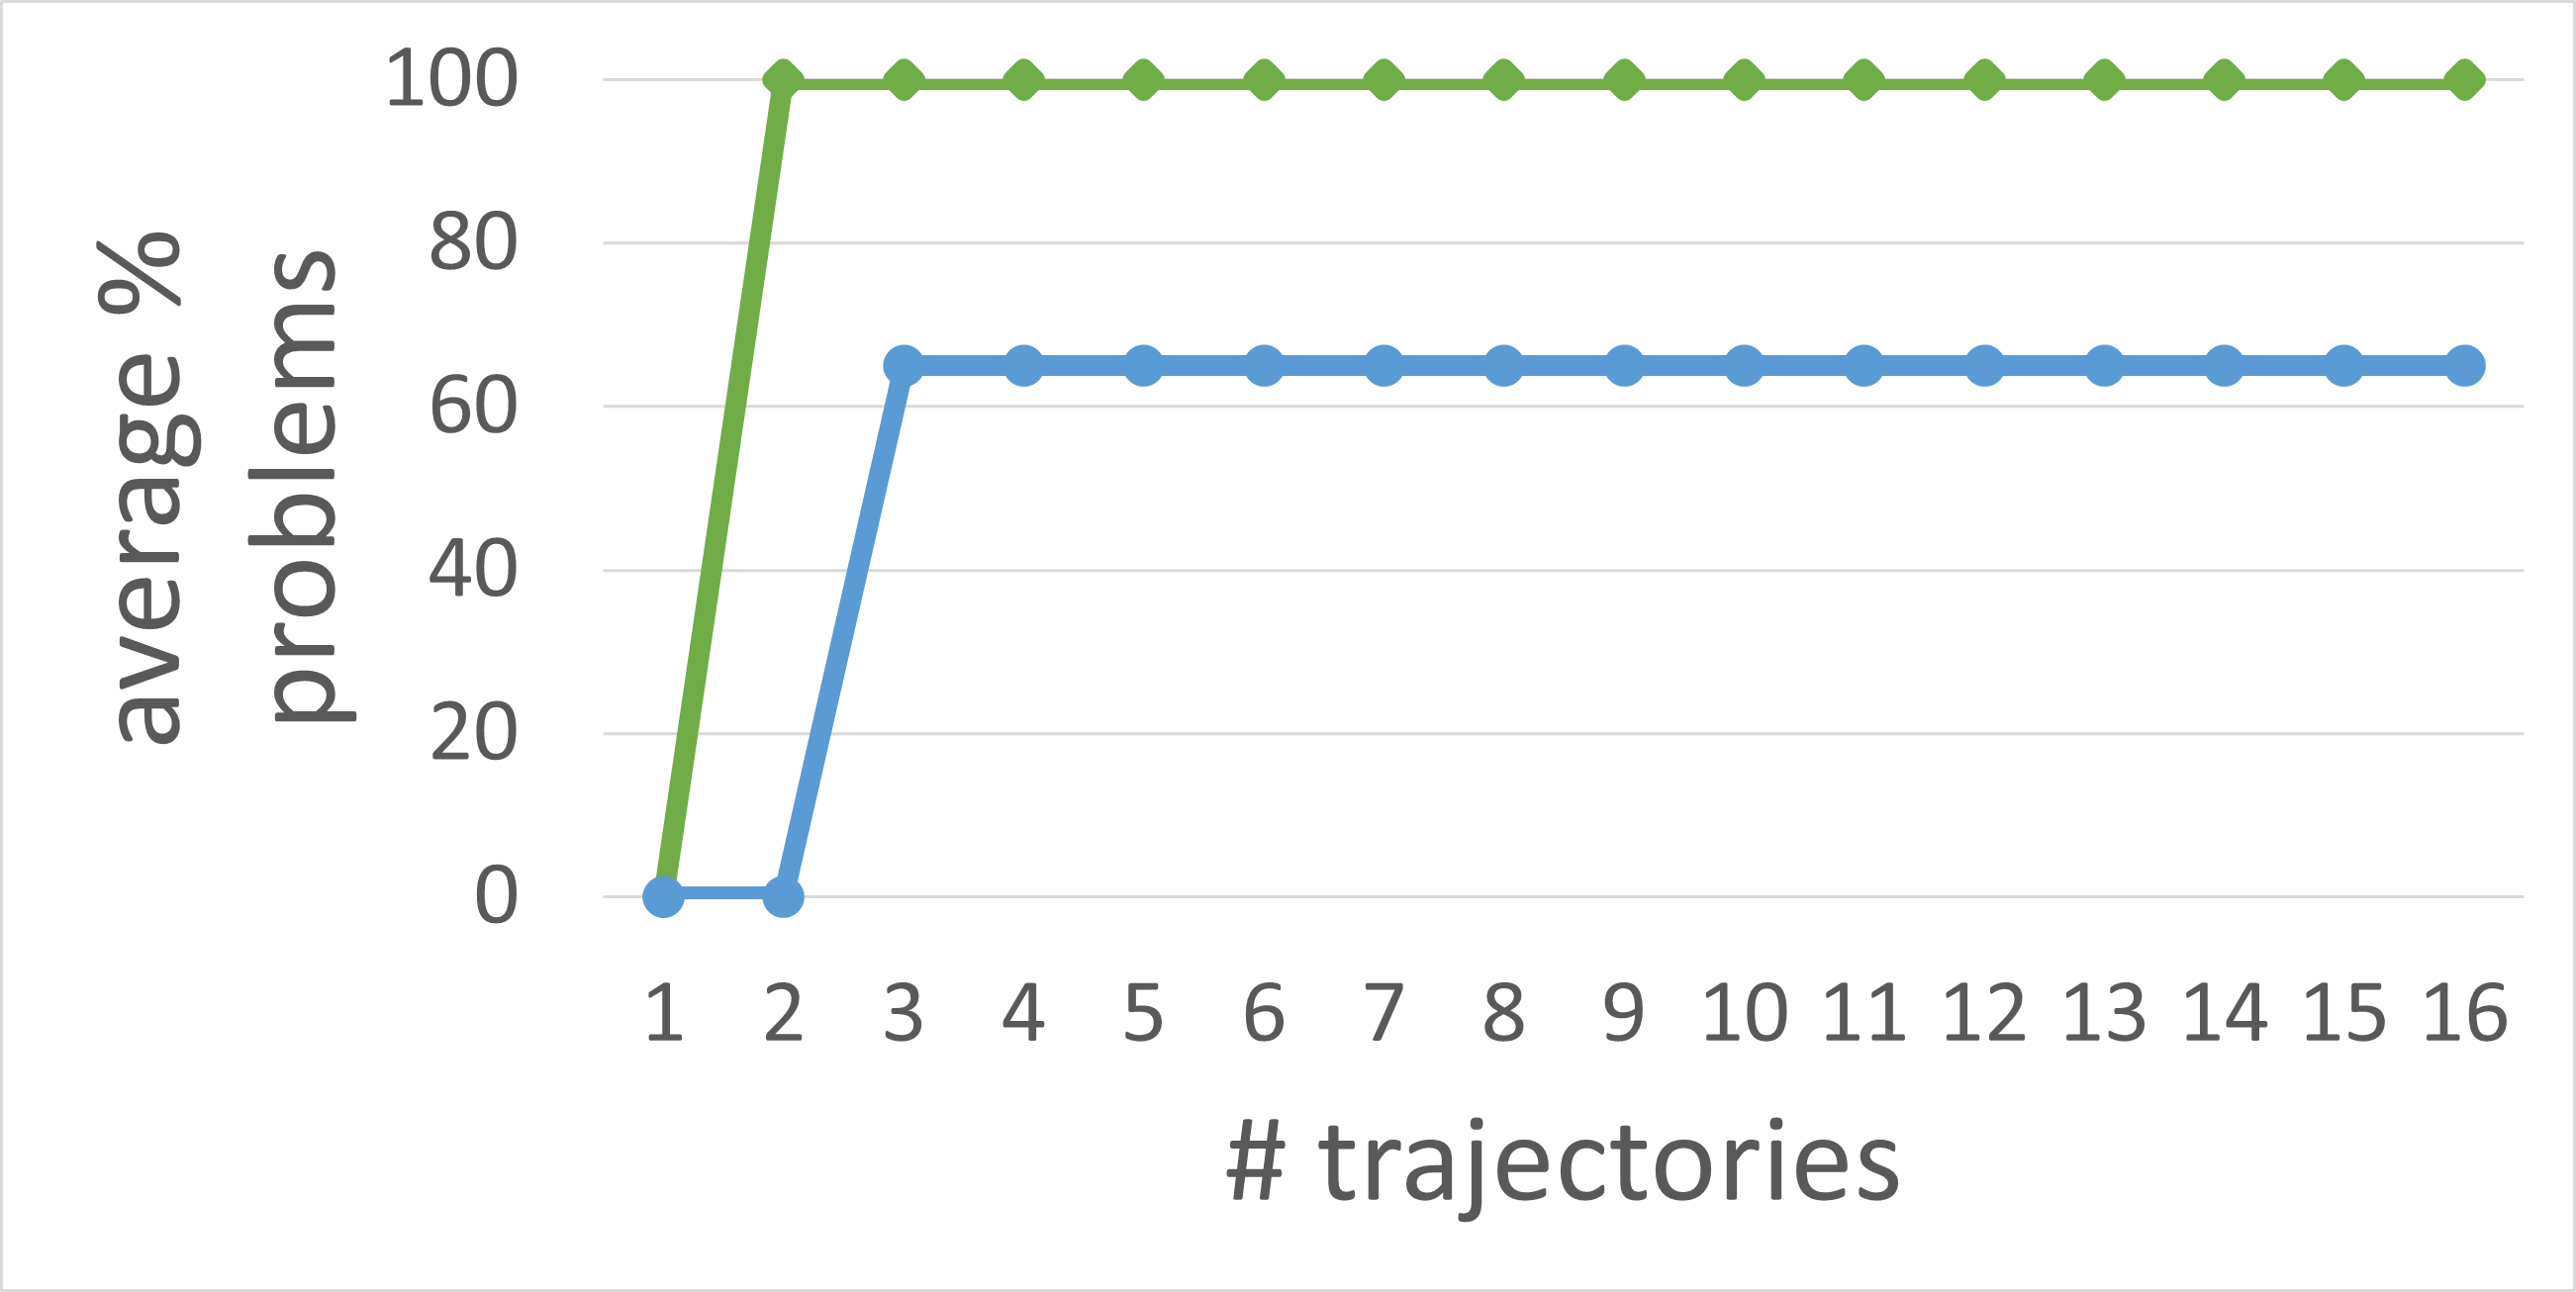
\includegraphics[width=0.48\columnwidth]{figures/logistics_hard_learning.png}
    \caption{Logistics}
    \label{fig:logistics-results}
  \end{subfigure}\\
  \begin{subfigure}[b]{\columnwidth}
    \centering
    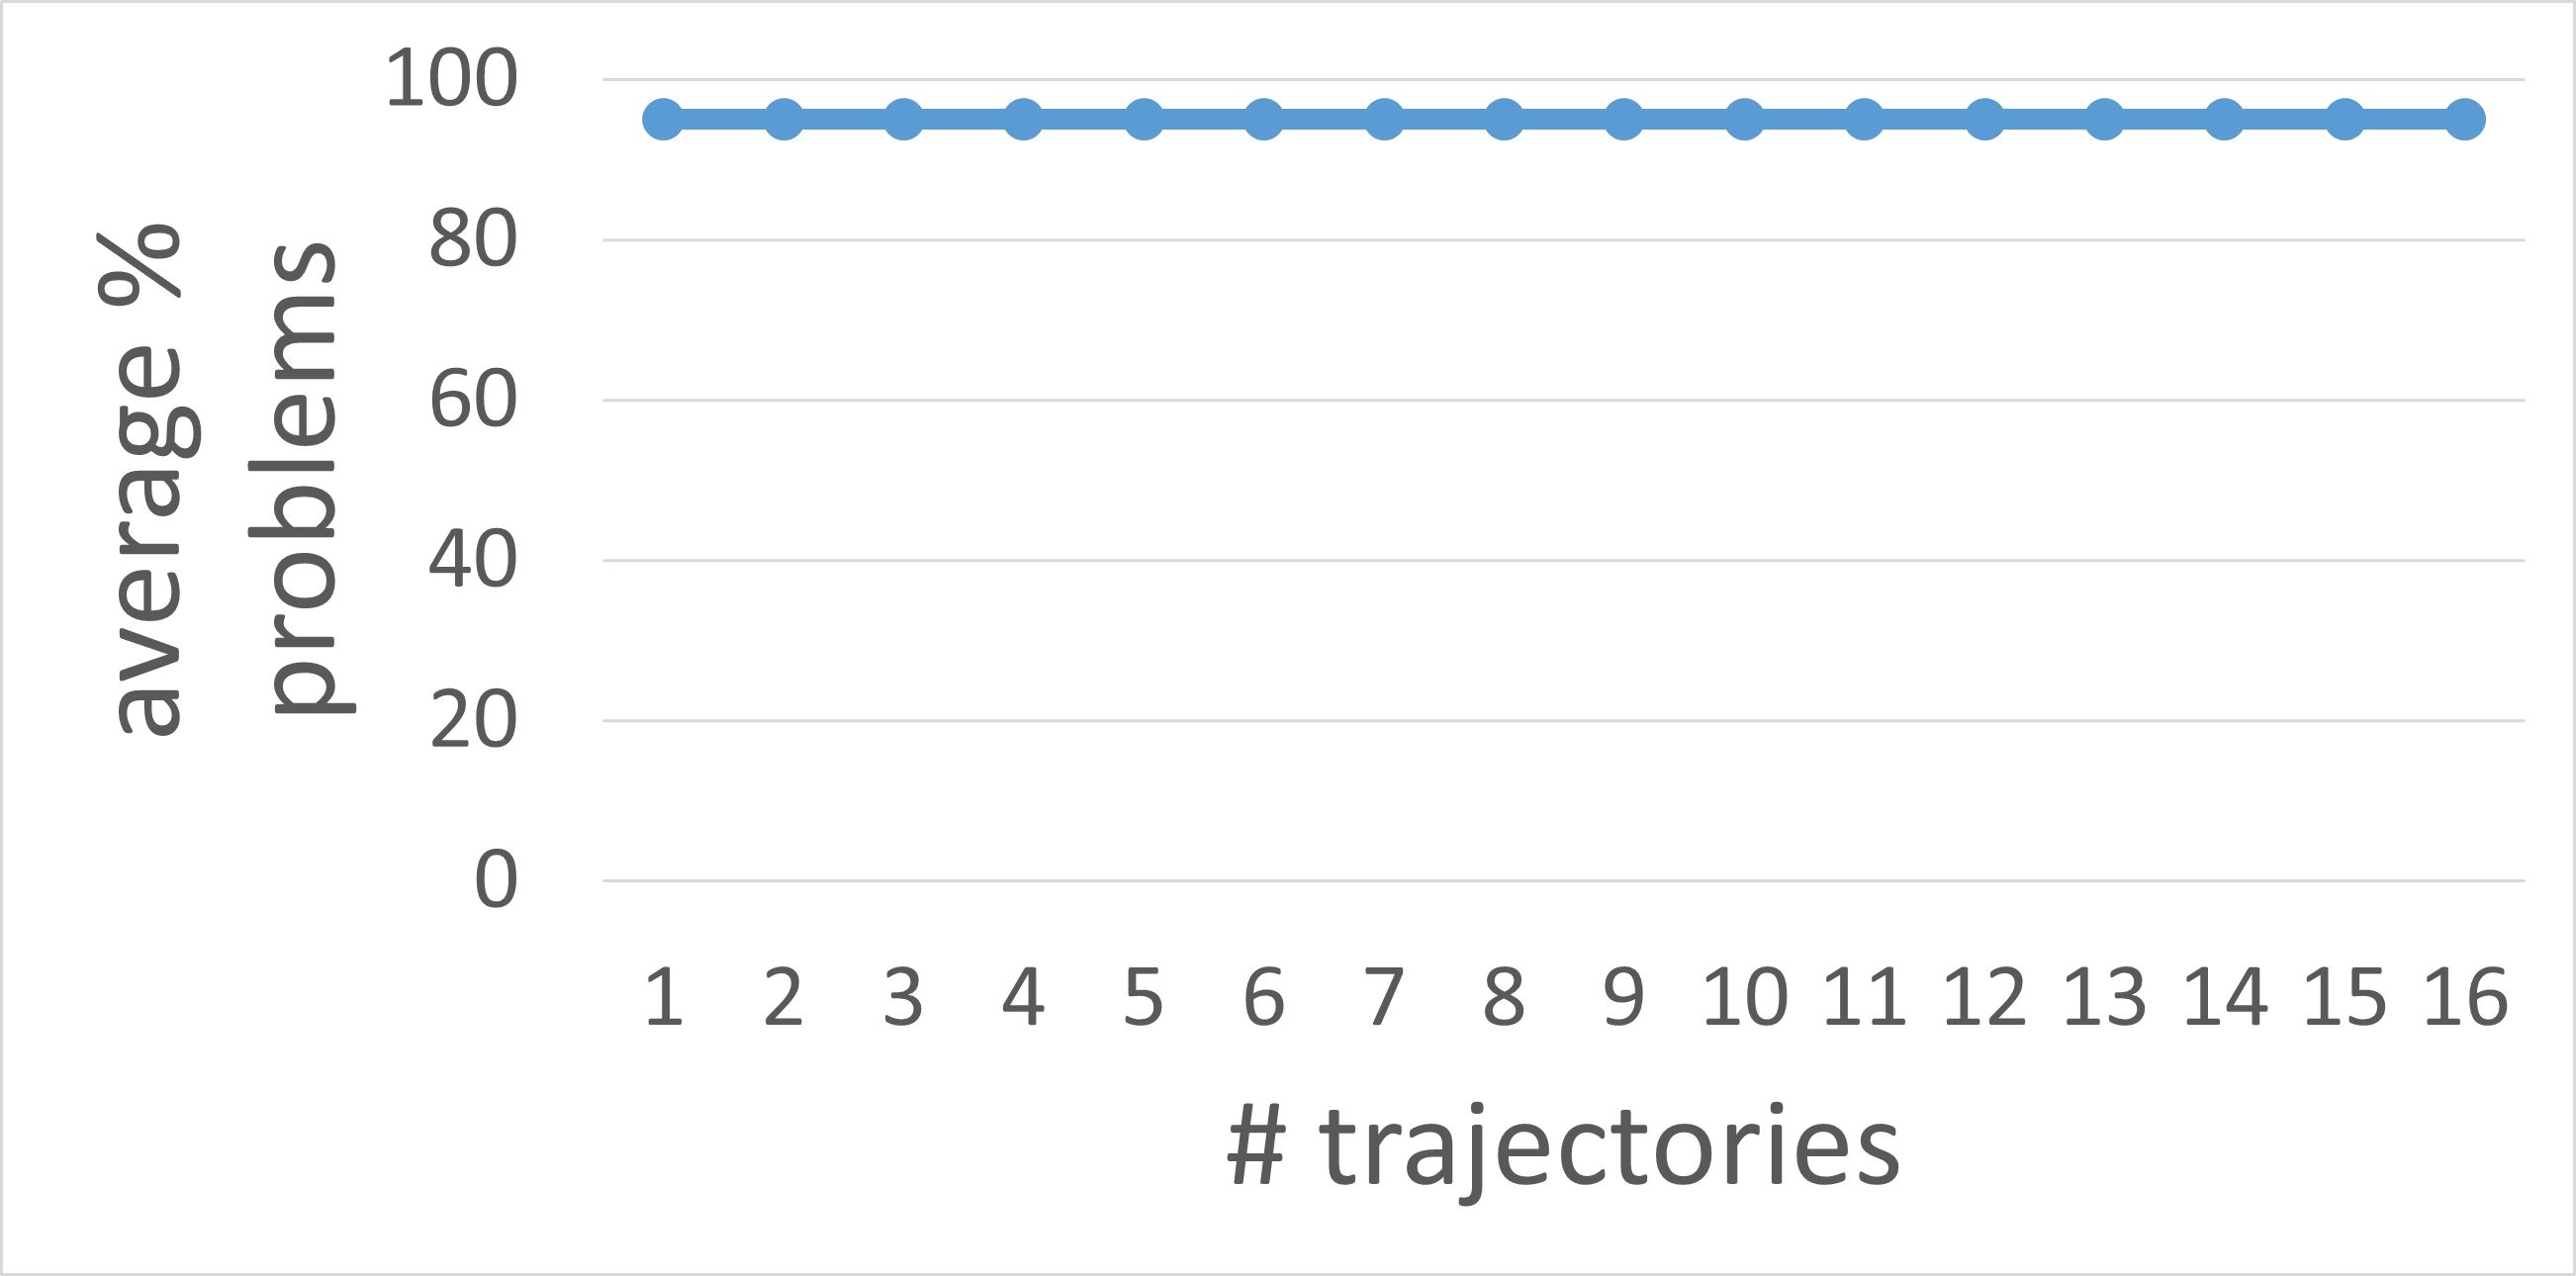
\includegraphics[width=0.48\columnwidth]{figures/blocks_easy_learning.png}
    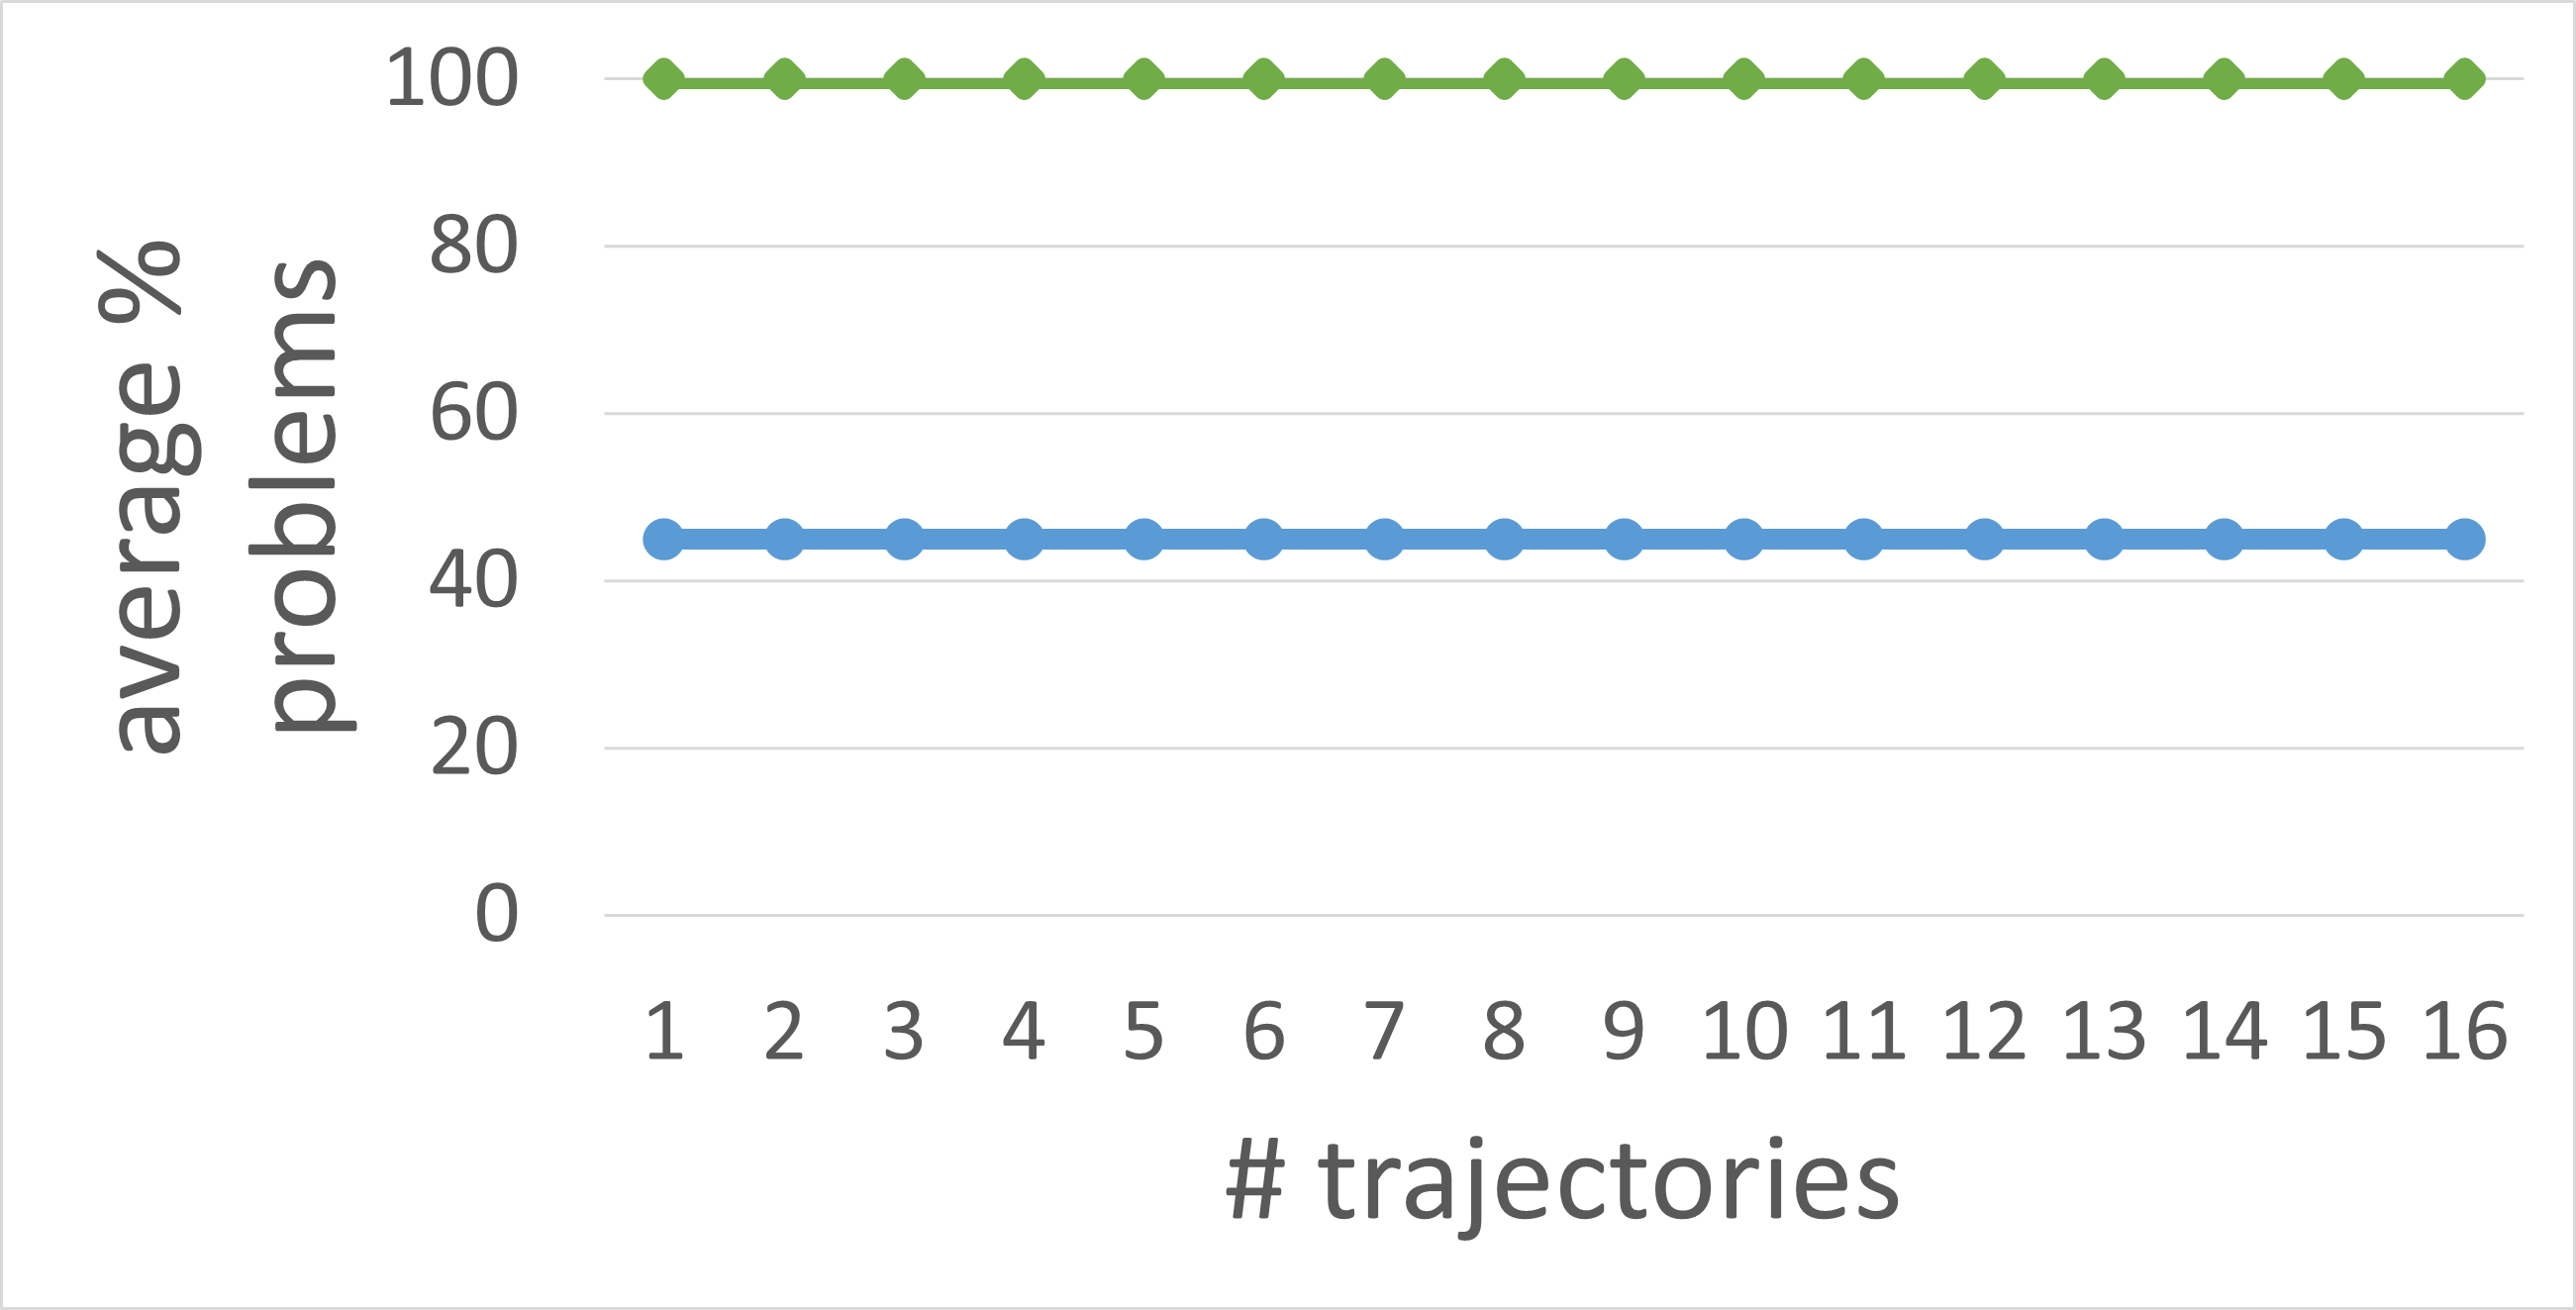
\includegraphics[width=0.48\columnwidth]{figures/blocks_hard_learning.png}
    \caption{Blocks}
    \label{fig:blocks-results}
  \end{subfigure}
  \caption{\% of the test set problems solved by \masam (green diamond) and \sam (blue circle) in each domain. (left) results without the additional actions to encourage concurrency. (right) results with encouraged concurrency.}
  \label{fig:solving-results}
\end{figure}


%\subsection{Benchmark domains}
%We experimented on domains from the publicly available CoDMAP benchmark~\cite{vstolba2016competition}.%\footnote{http://agents.fel.cvut.cz/codmap/}
\subsubsection{Generating trajectories of joint actions}
To generate trajectories for learning, we generated plans for the problems in the evaluated domain using two MA-STRIPS solvers: GPPP~\shortcite{maliah2017collaborative} with landmarks and FF heuristics and MAFS~\shortcite{nissim2014distributed} with the FF heuristic.
% We used this method to generate the input trajectories instead of random plans since we want our algorithm to learn the conditions for a successful execution of actions.
Like most existing MA-STRIPS solvers,
these MA-STRIPS solvers output a plan $\pi$ which is a sequence of single-agent actions.
To create trajectories with non-trivial joint actions, we grouped maximal consecutive sequences of single-agent actions that form well-defined joint actions~\cite{crosby2014single}.
% \begin{figure}
% \begin{center}
% \begingroup
%     \fontsize{8pt}{8pt}\selectfont
% \begin{Verbatim}[commandchars=\\\{\}]
% (:action dummy-add-predicate-action
%     :parameters (?agent - object)
%     :precondition (and)
%     :effect (and (dummy-additional-predicate)
%     )
% )

% (:action dummy-del-predicate-action
%     :parameters (?agent - object)
%     :precondition (and)
%     :effect (and (not (dummy-additional-predicate))
%     )
% )
% \end{Verbatim}
% \endgroup
% %removedVspace
% \caption{The new actions that were added to each agent's domain. The actions receive the agent as a parameter and add or delete the new predicate.}
% %removedVspace
% \label{list:new-actions-to-domain}
% \end{center}
% \end{figure}
% These trajectories were used in the first experimental setup.
In some domains, the resulting trajectories of joint actions contained fewer than 10\% action triplets with non-trivial joint actions, i.e., joint actions that include more than one action that is not a \noop.
Since our contribution is learning from \emph{concurrently executed actions}, we conducted a second set of experiments in which we modified the benchmark domain to encourage non-trivial joint actions. Specifically,
we added the predicate \textit{dummy-additional-predicate} with no parameters, and the agents' actions do not add or delete it.
Then, we added two new actions to each agent \textit{dummy-add-predicate-action} and \textit{dummy-del-predicate-action} that have no preconditions, and they add or delete the newly added predicate, respectively.
% Figure~\ref{list:new-actions-to-domain} presents the actions added to the agents' action models.
To create trajectories containing these new actions, we randomly added the new actions with the original ones to compose joint actions while the resulting plans remained well-defined.
We set the probability of adding one of the new actions to 0.65 for each joint action in the plan sequence.
This means, on average, at least 65\% of the transitions in our trajectories include a non-trivial joint action. %\roni{@Argaman, am I correct?}
We chose such a high percentage of non-trivial joint actions to challenge the algorithms and observe the necessity of supporting concurrency in multi-agent planning. %\roni{Why?}
% With the changes described above, we increased the number of non-trivial joint actions and the total number of actions in any joint action.
% \roni{Not clear how this allows more actions to be concurrent}
Finally, we randomly selected problems and added the newly defined predicate to the goal state.
This addition prevents a planner from solving problems unless the action model it uses includes actions that affect \textit{dummy-additional-predicate}, i.e., by learning from non-trivial joint actions.
% \roni{Why is this important? I think it is because this means we have to learn enough about the dummy actions to apply them}



Table~\ref{tab:domains-information} presents characteristics of the domains used in our experiments.
Columns $|A|$, $|P|$, $arity(p)$, $arity(a)$, ``max $|A_i|$'', and $|\mathcal{T}|$ contain the number of lifted actions (not including those newly added), the number of lifted fluents,  the maximum arity of fluents, the maximum arity of actions, the maximum number of agents acting in a problem, and the total number of trajectories available respectively.
Columns ``$|t|$'', ``\%SA$_1$'', and ``\%SA$_2$'' present the total number of action triplets in the training trajectories and the percentage of triplets that consist only of trivial joint actions.
%, i.e., include only single agent actions, in the first and second settings. REPETITION
% \roni{I do not think ``experimentation setting'' is the correct English term. I am not certain it's incorrect, but I know that ``experimental setup'' is commonly used}
% \roni{I wonder if showing the SA-t and SA*-T results as percentage of the MA-t wouldn't be clearer}
% While in most domains, only a few joint actions include concurrently executed actions, in some domains, such as Depots, the number of concurrent actions is significant (165 out of 500).

% \subsection{Experimental Setup}
% \label{sec:experimental-setup}




\begin{table}[ht]
\centering
\resizebox{\columnwidth}{!}{%
\begin{tabular}{|l|c|c|c|c|c|c|c|c|c|}
\hline
\multicolumn{1}{|c|}{\textbf{Domain}} &
\textbf{$|A|$} &
\textbf{$|P|$} &
\textbf{\begin{tabular}[c]{@{}c@{}}max \\ $arity(p)$\end{tabular}} &
\textbf{\begin{tabular}[c]{@{}c@{}}max \\ $arity(a)$\end{tabular}} &
\textbf{\begin{tabular}[c]{@{}c@{}}max \\ $|A_i|$\end{tabular}} &
\textbf{$|\mathcal{T}|$} &
\textbf{$|t|$}  &
\textbf{\%SA$_1$} &
\textbf{\%SA$_2$}\\ \hline
blocksworld & 4 & 5 & 2 & 3 & 4  & 20 & 1314    & 91   & 34 \\ \hline
depots      & 5 & 7 & 3 & 4 & 12 & 16 & 506     & 67   & 23 \\ \hline
driverlog   & 6 & 6 & 2 & 4 & 8  & 16 & 277     & 94   & 28 \\ \hline
logistics   & 5 & 6 & 3 & 4 & 7  & 20 & 686     & 74   & 26 \\ \hline
rovers      & 9 & 25 & 2 & 6 & 10  & 20 & 833   & 88   & 31  \\ \hline
satellite   & 5 & 8 & 2 & 4 & 10  & 20 & 1,053  & 99   & 35 \\ \hline
sokoban     & 3 & 6 & 3 & 6 & 4  & 11 & 406     & 78   & 29 \\ \hline
\end{tabular}%
}
\caption{Characteristics of the domains in our experiments.}% The domains were extracted from the CoDMAP benchmark.}
\label{tab:domains-information}
\end{table}




% UP TO HERE
\subsubsection{Evaluation Metrics}
We measured the number of problems solved with the learned action model
and the precision and recall of the learned action model.
To measure the number of problems solved,
we ran Fast-Downward~\cite{helmert2006fast} with
the learned action model and counted the number of problems solved within a time limit of 60 seconds. % for each problem.
% If the problem has not been solved within this time frame or the planner de, the solver will return that a "time-out" had occurred.
In our experiments, we observed that the effects are learned perfectly and very quickly, and , we focus on preconditions' precision and recall.
We distinguish between the \textit{syntactic} precision and recall of the preconditions and their \textit{semantic} precision and recall, denoted by $P^{syn}_\pre$, $R^{syn}_\pre$, $P^{sem}_\pre$ and $R^{sem}_\pre$ respectively.
The syntactic precision and recall values measure the textual difference between the real and learned domains.
These metrics may be misleading as two action models may be different syntactically yet still allow solving the same number of problems.
The \textit{semantic precision and recall} of the preconditions address this limitation and is computed as follows:
%Similarly, $applicable_{M^*}(a)$ is the set of states in which $a$ is applicable according to \realm.
%We define another metric to evaluate the accuracy of the learned domains.
%We refer to this metric as \textit{semantic precision/recall}.
%We calculate the semantic precision and recall for each action as follows:
\begin{align*}\small
    P^{sem}_{\pre}(a)= \frac{|app_{\realm}(a)\cap app_M(a)|}{|app_M(a)|} \\
    R^{sem}_{\pre}(a)= \frac{|app_{\realm}(a)\cap app_M(a)|}{|app_{\realm}(a)|}
\end{align*}
where $app_M(a)$ denotes the states in a set of trajectories where $a$ is applicable according to the action model $M$.
Since \masam learns a safe action model, the syntactic recall and the semantic precision are always 1, so we only present results for syntactic precision and semantic recall.
There is no natural baseline to compare with \masam since all other works on learning action models do not support learning from trajectories with joint actions.
Thus, as a baseline, we compared \masam with the single-agent \sam algorithm, which can only learn from action triplets in which the joint action contains exactly one action.
%in the joint action. This baseline is fundamentally the basic, single-agent \sam algorithm.
% For both values, we report the average value over all actions.

% To evaluate the semantic precision and recall over the entire action model, we average the semantic precision and recall of all actions.


% Since we learn a safe action model, the preconditions of the learned action model is a superset of the ones in the real action model. Thus, the recall value of the actions' preconditions is also 1.



\subsubsection{Results}
\label{sec:results}
% We compared the averaged number of problems solved by \masam and \sam in both settings. REPETITION

Figure~\ref{fig:solving-results} presents the average percentage of problems solved as the number of input trajectories varies for each domain in both settings.
In the first experiment, in all domains except Rovers, both \masam and \sam were eventually able to solve over 85\% of the test problems.
In Blocksworld and Logistics, both algorithms learned a correct action model after one trajectory and solved almost all test problems.
The results on Driverlog, Depots, Sokoban, and Rovers highlight that  \masam learns faster than \sam, as expected. %since it utilizes more knowledge. % than \sam.
% This trend can be observed in Driverlog, Depts, and Sokoban Domains.
The weaker performance of both algorithms on Rovers is due to the size of the domain: it has significantly more lifted fluents and actions than all other domains.
The advantage of \masam over \sam is highlighted by the results on the second set of experiments, shown in Figure~\ref{fig:solving-results} (right).
%, where non-trivial joint actions were encouraged (Figure~\ref{fig:solving-results} (right)).
% In the second setting, where non-trivial joint actions were encouraged, we observed that adding \textit{dummy-additional-predicate} to the goal state of the test set problems affected the results for \sam since it could never learn the actions that add it.
For example, in Blocksworld, \sam could not solve more than 45\% of the test problems while \masam had 100\% success.
% This result correlates with the percentage of goals changed with the additional predicate.  In addition, we can see that the small number of single-agent action triplets affected the learning rate. In Depots, Driverlog, Satellite, and Logistics domains \sam requires more trajectories than \masam to converge.

% Note that the Rovers
% We observe that some of the learned actions for the Rovers domain contain more preconditions in the domains generated by \sam than those generated by \masam.
% These additional preconditions explain the results in Figure~\ref{fig:rovers-results}.
% We note that the Rovers domain contains more actions and predicates than the other domains, making it much harder to learn. Thus,  both \sam and \masam fail to learn a representation that enables solving all test set problems.


% We notice that when we did not inject additional actions, the average percentage of problems solved is similar for both \sam and \masam for most domains
% \roni{Danger: a reviewer may say ``ah, so we didn't really need MA-SAM in practice'' try to say differently}.
% After the learning converges for Sokoban, Drivelog, and Depots domains, both algorithms output the same results.


% \roni{The results will be clearer if you split to first discuss the results for the first experiment, and then the results of the other. Currently it is convoluted which makes reading hard.}
% In Blocksworld, Logistics, Satellite, and DriverLog, \masam  was able to solve almost all test problems with only a single trajectory learning, and all of them with only two trajectories.
% Figure~\ref{fig:problem-solved-graphs} shows the average percentage of problems solved in each of the remaining domains as a function of the number of given trajectories.
% The results show that \masam can learn a more robust action model faster (i.e., with fewer trajectories) than the baseline algorithm. For example, in the Depots domain, \masam learned an action model strong enough to solve all problems using only one trajectory, whereas the baseline required 3 trajectories.  %The same trend applies to the Driverlog domain as well.


% In the Blocksworld domain, except for a single fold, the planner solved all test set problems. In the outlier fold, it timed out on a single problem for any given number of trajectories.
% In the Logistics domain, the planner solved all the test set problems in all folds.
% In the Satellite domain, we observed an identical behavior for the two versions of \masam.
% For both algorithms using one trajectory, the solver solved 95\% problems, and after two trajectories, all test set problems were solved.
% For this reason, we decided not to present these three domains graphically.


% % Figure~\ref{fig:problem-solved-graphs} shows the average percentage of problems solved over the 5-fold, in each domain, as a function of the number of train set trajectories and the learning algorithm.
% Figure~\ref{fig:problem-solved-graphs} shows the average percentage of problems solved in each domain as a function of the number of trajectories. % and the learning algorithm.
% We differentiate the results on the type of learning algorithm that created the domains used to solve the test set problems, i.e., \masam and its baseline version.




\begin{table}[ht]
\centering
\resizebox{0.45\columnwidth}{!}{%
\begin{tabular}{|l|c|c|}
\hline
\multicolumn{1}{|c|}{\textbf{Domain}} & \textbf{$P^{syn}_\pre$}  & \textbf{$R^{sem}_\pre$}  \\ \hline
Blocksworld & 0.60 &  1.00\\ \hline
Depots      & 0.68 &  1.00\\ \hline
Driverlog   & 0.59 &  1.00\\ \hline
Logistics   & 0.66 &  1.00\\ \hline
Rovers      & 0.62 &  0.88\\ \hline
Satellite   & 0.70 &  0.99\\ \hline
Sokoban     & 0.68 &  0.99\\ \hline
\end{tabular}%
}
\caption{Average syntactic precision and semantic recall of actions' preconditions.}% and the semantic precision and recall of each domain when using the maximal number of trajectories.
\label{tab:precision-recall}
\end{table}



% \begin{table}[ht]
% \centering
% \resizebox{0.5\columnwidth}{!}{%
% \begin{tabular}{|l|c|c|}
% \hline
% \multicolumn{1}{|c|}{\textbf{Domain}} & \textbf{$P^{syn}_\pre$}  & \textbf{$R^{sem}_\pre$}  \\ \hline
% Blocksworld & 0.41 &  1.00\\ \hline
% Depots      & 0.56 &  1.00\\ \hline
% Driverlog   & 0.48 &  1.00\\ \hline
% Logistics   & 0.55 &  1.00\\ \hline
% Rovers      & 0.54 &  0.85\\ \hline
% Satellite   & 0.59 &  0.98\\ \hline
% Sokoban     & 0.68 &  1.00\\ \hline
% \end{tabular}%
% }
% \caption{Average syntactic precision and semantic recall of actions' preconditions.}% and the semantic precision and recall of each domain when using the maximal number of trajectories.
% \label{tab:precision-recall}
% \end{table}

%In our experimentation, we observed that the effects' syntactic precision and recall values are constant 1.

Table~\ref{tab:precision-recall} shows the average syntactic precision and semantic recall for preconditions ($P^{syn}_\pre$ and $R^{sem}_\pre$) for the action model learned by \masam for every domain given all the available trajectories. We show results only for the second set of experiments since it presented more challenges to both algorithms. Interestingly, the syntacicantly different.
This difference highlights that while \masam's conservative approach to learning preconditions indeed learns more preconditions than those appearing in the PDDL domain, in most cases, these additional preconditions do not affect the 
Here too, Rovers pose the greatest challenge to \masam 
% For example, in the Blocksworld domain \masam included three additional literals as preconditions for the \textit{put-down} action, \textit{(not (ontable ?x))}, \textit{(not (handempty ?a))} and \textit{(not (clear ?x))}. The only precondition required, according to the PDDL definition, is \textit{(holding ?a ?x)}. The additional three literals, however, are always true when \textit{(holding ?a ?x)} is true, and  adding them does not limit the set of problems that can be solved with the learned action model. [[Roni: omitted for space]]

% That being said, in some cases \masam does learn a restrictive model that is weaker than the original PDDL domain.
% Such cases are presented in the Satellite, Sokoban and Rovers domains.
% In the Satellite and Sokoban domains, we can see that the semantic recall is 99\% which indicates that the number of states in which an action would be inapplicable, compared to the real action, is very small.
% In the Rovers domain, on the other hand, we can see that the semantic recall is only 88\% which is relatively low.
% This indicates that some solvable problems might not be solved using \masam's learned domains since they are too restrictive. [[Roni: omitted for space]]

%We also evaluated our algorithm by calculating the total percentage of test set problems solved. We compared these findings with a baseline version of \masam where action triplets.



% We examined more metrics for the Sokoban and Rovers domains to better understand the algorithms' behavior given different numbers of trajectories.
% Table~\ref{tab:learning-rate} displays the average number of preconditions learned for each action model in column \pre, the average number of safe actions in the column ``safe'', and then the average percentile of the unsolvable problems and those which the solver timed out in the columns ``NS'' and ``TO'', respectively.

% In the Sokoban domain, for all trajectories, all actions were considered safe for both \masam and the baseline algorithm.
% Furthermore, using one trajectory, both \masam and the baseline version performed the same.
% Once adding a second trajectory, we observe the benefits of learning from joint actions with multiple single-agent actions.
% \masam eliminates more preconditions than the baseline algorithm, and as a result, more problems are solved using the model generated by \masam. This indicates that once the action model created is too restrictive; the test set problems become unsolvable.
% We notice that this trend continues until both algorithms learn the same action model after four trajectories.

% In  Rovers, we observe that the average number of safe actions learned by \masam is lower than that of the baseline algorithm for one trajectory.
% This means that \masam encountered a concurrent execution of actions that resulted in ambiguity.
% However, no problem was solved for either algorithm since some required actions were missing from the model.
% From two trajectories onward, both algorithms learn all the actions.
% Similarly to the Sokoban domain, \masam creates a concise action model with fewer preconditions, and  more test set problems become solvable.

% These observations show \masam performs as well as or better than when ignoring triplets containing multiple actions.
% These results signify the importance of learning from triplets containing concurrent execution of actions.

% Please add the following required packages to your document preamble:
% \usepackage{graphicx}
% \begin{table}[]
% \centering
% \resizebox{\columnwidth}{!}{%
% \begin{tabular}{|c|cccc|cccc|}
% \hline
%  &
%   \multicolumn{4}{c|}{MA-SAM} &
%   \multicolumn{4}{c|}{Baseline} \\ \hline
% $|\mathcal{T}|$ &
%   \multicolumn{1}{c|}{\pre} &
%   \multicolumn{1}{c|}{safe} &
%   \multicolumn{1}{c|}{NS} &
%   TO &
%   \multicolumn{1}{c|}{\pre} &
%   \multicolumn{1}{c|}{safe} &
%   \multicolumn{1}{c|}{NS} &
%   TO \\ \hline
% 1 &
%   \multicolumn{1}{c|}{14.64} &
%   \multicolumn{1}{c|}{7.40} &
%   \multicolumn{1}{c|}{100} &
%   0 &
%   \multicolumn{1}{c|}{16.00} &
%   \multicolumn{1}{c|}{8.20} &
%   \multicolumn{1}{c|}{100} &
%   0 \\ \hline
% 2 &
%   \multicolumn{1}{c|}{11.80} &
%   \multicolumn{1}{c|}{9.00} &
%   \multicolumn{1}{c|}{35} &
%   15 &
%   \multicolumn{1}{c|}{12.62} &
%   \multicolumn{1}{c|}{9.00} &
%   \multicolumn{1}{c|}{65} &
%   15 \\ \hline
% 3 &
%   \multicolumn{1}{c|}{11.22} &
%   \multicolumn{1}{c|}{9.00} &
%   \multicolumn{1}{c|}{30} &
%   0 &
%   \multicolumn{1}{c|}{11.69} &
%   \multicolumn{1}{c|}{9.00} &
%   \multicolumn{1}{c|}{55} &
%   0 \\ \hline
% 4 &
%   \multicolumn{1}{c|}{10.96} &
%   \multicolumn{1}{c|}{9.00} &
%   \multicolumn{1}{c|}{30} &
%   0 &
%   \multicolumn{1}{c|}{11.27} &
%   \multicolumn{1}{c|}{9.00} &
%   \multicolumn{1}{c|}{40} &
%   0 \\ \hline
% 5 &
%   \multicolumn{1}{c|}{10.71} &
%   \multicolumn{1}{c|}{9.00} &
%   \multicolumn{1}{c|}{30} &
%   0 &
%   \multicolumn{1}{c|}{10.99} &
%   \multicolumn{1}{c|}{9.00} &
%   \multicolumn{1}{c|}{30} &
%   0 \\ \hline
% \end{tabular}%
% }
% \caption{Rovers domain comparison of the learning rate of both \masam and the baseline algorithm. }
% \label{tab:rovers-learning-rate}
% \end{table}

% % Please add the following required packages to your document preamble:
% % \usepackage{graphicx}
% \begin{table}[]
% \centering
% \resizebox{\columnwidth}{!}{%
% \begin{tabular}{|c|cccc|cccc|}
% \hline
% \multicolumn{1}{|c|}{} &
%   \multicolumn{4}{c|}{MA-SAM} &
%   \multicolumn{4}{c|}{Baseline} \\ \hline
% $|\mathcal{T}|$ &
%   \multicolumn{1}{c|}{\pre} &
%   \multicolumn{1}{c|}{safe} &
%   \multicolumn{1}{c|}{NS} &
%   \multicolumn{1}{c|}{TO} &
%   \multicolumn{1}{c|}{\pre} &
%   \multicolumn{1}{c|}{safe} &
%   \multicolumn{1}{c|}{NS} &
%   \multicolumn{1}{c|}{TO} \\ \hline
% 1 &
%   \multicolumn{1}{l|}{15.07} &
%   \multicolumn{1}{l|}{3} &
%   \multicolumn{1}{l|}{60} &
%   10 &
%   \multicolumn{1}{l|}{15.07} &
%   \multicolumn{1}{l|}{3} &
%   \multicolumn{1}{l|}{60} &
%   10 \\ \hline
% 2 &
%   \multicolumn{1}{l|}{13.73} &
%   \multicolumn{1}{l|}{3} &
%   \multicolumn{1}{l|}{40} &
%   10 &
%   \multicolumn{1}{l|}{14.53} &
%   \multicolumn{1}{l|}{3} &
%   \multicolumn{1}{l|}{60} &
%   10 \\ \hline
% 3 &
%   \multicolumn{1}{l|}{13.13} &
%   \multicolumn{1}{l|}{3} &
%   \multicolumn{1}{l|}{20} &
%   17 &
%   \multicolumn{1}{l|}{13.20} &
%   \multicolumn{1}{l|}{3} &
%   \multicolumn{1}{l|}{30} &
%   17 \\ \hline
% 4 &
%   \multicolumn{1}{l|}{12.60} &
%   \multicolumn{1}{l|}{3} &
%   \multicolumn{1}{l|}{20} &
%   17 &
%   \multicolumn{1}{l|}{12.60} &
%   \multicolumn{1}{l|}{3} &
%   \multicolumn{1}{l|}{20} &
%   17 \\ \hline
% 5 &
%   \multicolumn{1}{l|}{12.47} &
%   \multicolumn{1}{l|}{3} &
%   \multicolumn{1}{l|}{20} &
%   17 &
%   \multicolumn{1}{l|}{12.47} &
%   \multicolumn{1}{l|}{3} &
%   \multicolumn{1}{l|}{20} &
%   17 \\ \hline
% \end{tabular}%
% }
% \caption{Sokoban domain comparison of the learning rate of both \masam and the baseline algorithm.}
% \label{tab:sokoban-learning-rate}
% \end{table}



% \begin{table}[]
% \centering
% \resizebox{0.9\columnwidth}{!}{%
% \begin{tabular}{|c|cccc|cccc|}
% \hline
%  &
%   \multicolumn{4}{c|}{MA-SAM} &
%   \multicolumn{4}{c|}{Baseline} \\ \hline
% & \multicolumn{8}{|c|}{Rovers}\\ \hline
% $|\mathcal{T}|$ &
%   \multicolumn{1}{c|}{\pre} &
%   \multicolumn{1}{c|}{safe} &
%   \multicolumn{1}{c|}{NS} &
%   TO &
%   \multicolumn{1}{c|}{\pre} &
%   \multicolumn{1}{c|}{safe} &
%   \multicolumn{1}{c|}{NS} &
%   TO \\ \hline
% 1 &
%   \multicolumn{1}{c|}{14.64} &
%   \multicolumn{1}{c|}{7.40} &
%   \multicolumn{1}{c|}{100} &
%   0 &
%   \multicolumn{1}{c|}{16.00} &
%   \multicolumn{1}{c|}{8.20} &
%   \multicolumn{1}{c|}{100} &
%   0 \\ \hline
% 2 &
%   \multicolumn{1}{c|}{11.80} &
%   \multicolumn{1}{c|}{9.00} &
%   \multicolumn{1}{c|}{35} &
%   15 &
%   \multicolumn{1}{c|}{12.62} &
%   \multicolumn{1}{c|}{9.00} &
%   \multicolumn{1}{c|}{65} &
%   15 \\ \hline
% 3 &
%   \multicolumn{1}{c|}{11.22} &
%   \multicolumn{1}{c|}{9.00} &
%   \multicolumn{1}{c|}{30} &
%   0 &
%   \multicolumn{1}{c|}{11.69} &
%   \multicolumn{1}{c|}{9.00} &
%   \multicolumn{1}{c|}{55} &
%   0 \\ \hline
% 4 &
%   \multicolumn{1}{c|}{10.96} &
%   \multicolumn{1}{c|}{9.00} &
%   \multicolumn{1}{c|}{30} &
%   0 &
%   \multicolumn{1}{c|}{11.27} &
%   \multicolumn{1}{c|}{9.00} &
%   \multicolumn{1}{c|}{40} &
%   0 \\ \hline
% 5 &
%   \multicolumn{1}{c|}{10.71} &
%   \multicolumn{1}{c|}{9.00} &
%   \multicolumn{1}{c|}{30} &
%   0 &
%   \multicolumn{1}{c|}{10.99} &
%   \multicolumn{1}{c|}{9.00} &
%   \multicolumn{1}{c|}{30} &
%   0 \\ \hline

% & \multicolumn{8}{|c|}{Sokoban}\\
% \hline
% % \multicolumn{1}{|c|}{} &
% %   \multicolumn{4}{c|}{MA-SAM} &
% %   \multicolumn{4}{c|}{Baseline} \\ \hline
% $|\mathcal{T}|$ &
%   \multicolumn{1}{c|}{\pre} &
%   \multicolumn{1}{c|}{safe} &
%   \multicolumn{1}{c|}{NS} &
%   \multicolumn{1}{c|}{TO} &
%   \multicolumn{1}{c|}{\pre} &
%   \multicolumn{1}{c|}{safe} &
%   \multicolumn{1}{c|}{NS} &
%   \multicolumn{1}{c|}{TO} \\ \hline
% 1 &
%   \multicolumn{1}{l|}{15.07} &
%   \multicolumn{1}{l|}{3} &
%   \multicolumn{1}{l|}{60} &
%   10 &
%   \multicolumn{1}{l|}{15.07} &
%   \multicolumn{1}{l|}{3} &
%   \multicolumn{1}{l|}{60} &
%   10 \\ \hline
% 2 &
%   \multicolumn{1}{l|}{13.73} &
%   \multicolumn{1}{l|}{3} &
%   \multicolumn{1}{l|}{40} &
%   10 &
%   \multicolumn{1}{l|}{14.53} &
%   \multicolumn{1}{l|}{3} &
%   \multicolumn{1}{l|}{60} &
%   10 \\ \hline
% 3 &
%   \multicolumn{1}{l|}{13.13} &
%   \multicolumn{1}{l|}{3} &
%   \multicolumn{1}{l|}{20} &
%   17 &
%   \multicolumn{1}{l|}{13.20} &
%   \multicolumn{1}{l|}{3} &
%   \multicolumn{1}{l|}{30} &
%   17 \\ \hline
% 4 &
%   \multicolumn{1}{l|}{12.60} &
%   \multicolumn{1}{l|}{3} &
%   \multicolumn{1}{l|}{20} &
%   17 &
%   \multicolumn{1}{l|}{12.60} &
%   \multicolumn{1}{l|}{3} &
%   \multicolumn{1}{l|}{20} &
%   17 \\ \hline
% 5 &
%   \multicolumn{1}{l|}{12.47} &
%   \multicolumn{1}{l|}{3} &
%   \multicolumn{1}{l|}{20} &
%   17 &
%   \multicolumn{1}{l|}{12.47} &
%   \multicolumn{1}{l|}{3} &
%   \multicolumn{1}{l|}{20} &
%   17 \\ \hline
% \end{tabular}%
% }
% \caption{Comparing the learning rate of both \masam and the baseline algorithm, for Rovers and Sokoban.}
% \label{tab:learning-rate}
% \end{table}



% we can see that on average, when given only one trajectory to the baseline algorithm only 20\% of the problems were solved and the rest of the test set problems had no solution with the generated domain.
% On the other hand when we used \masam 85\% of the problems were solved and validated. When given two trajectories, the baseline algorithm improved to have 75\% of the problems solved and validated with only 20\% of the problems without a possible solution. From three trajectories onward both algorithms behaved the same with 95\% of the problems solved. We observed that with 16 trajectories, all of the test set problems were solved in all folds.

% In Driverlog domain we observed similar trends.
% Given one trajectory the \masam's domains can solve 73\% of the problems whereas with the baseline's domains no problem was solvable. From two trajectories both versions behaved the same converging on 100\% after three trajectories.
% In Sokoban domain we observed that when given a single trajectory \masam is able to solve 47\% of the problems, 37\% of the problems had no solution and for 16\% of the problems the solver timed out.
% On the other hand, using the baseline algorithm only 27\% of the test set problems were solved, 57\% had no solution and the rest (16\%) had timed out.
% \textbf{ROVERS NEEDS TO BE COMPLETED AND ADDED!!!}








% \section{Stuff to talk about}
% Definitions:
% lifted(l1,a1) = the parameter bound literal bounded by a1
% lifted(a1) = the lifted action for the grounded action a1
% lifted(l1) = the lifted literal for the grounded literal l1
% relevant(a,l) = the set of grounded actions in the joint action a that
% are bound to the grounded literal l.
% relevant(a) = the set

% Example:
% fluents: f1
% actions: a1,a2

% Observation 1:
% (not(f1), (a1,a2), f1)

% Observation 2:
% (not(f1), (a1,a3), not(f1))

% ==>
% pre(lifted(a1)) = not(lifted(f1,a1))
% pre(lifted(a2)) = not(lifted(f1,a2))

% CNF_{eff}(lifted(f1)) = ( is_eff(lifted(f1, a1), lifted(a1))
%                 or is_eff(lifted(f1, a2),a2) )

% General rules:
% For every transition (s,a,s'):
% 1.  For every literal $l\notin s$ and every $a'\in relevant(a,l)$
%     remove lifted(l,a') from pre(lifted(a')).

% 2.  For every literal $l\notin s'$ and every $a'\in relevant(a,l)$
%     add $\neg(\iseff(lifted(l,a'),lifted(a'))$ to $CNF_{lifted(l)}$

% 3.  For every literal $l\in s'\setminus s$
%     add $\bigvee_{a'\in relevant(a,l)} \iseff(lifted(l,a'),lifted(a'))$ to $CNF_{lifted(l)}$


% % Identify single-agent actions that have unambiguous effects
% When can we perform a lifted single-agent action $a$?
% If for every lifted literal $l$ and every parameter-bound literal $l'$ connecting $l$ and $a$
% either $CNF_{l}\rightarrow \iseff(l',a)$
% or $CNF_{l}\rightarrow \neg\iseff(l',a)$.

% <-- STOP HERE FOR EXPERIMENTS -->


% % Identify pairs of single-agent actions that have unambiguous effects when performed concurrently
% OPEN CHALLENGE
% When can we perform a joint action with a pair of single-agent actions (a1,a2)?
% If for every parameter-bound lifted literal $l$
% either $CNF_{l}\rightarrow (\iseff(l,a1)\vee \iseff(l,a2))$
% or $CNF_{l}\rightarrow \neg(\iseff(l,a1)\vee \iseff(l,a2))$.



% When can we perform a

% What is the effect of

% =========


% Algorithm:

% 1. For every transitions apply rules
% 2. For every CNF, minimize it (apply unit propagation)
%   (For every unit clause $l_\iseff$ in $CNF_X$, remove $\neg l_\iseff$ from all clauases in $CNF_X$)
% 3. SafeActions$\gets$ all lifted actions
% 4. For every lifted action $a$
% 3.1. For every parameter-bound lifted literal $l$ that can be relevant to $a$ and $l$ is not in $pre(a)$
% 3.1.1. If $\iseff(l,a)$ is not a unit clause in $CNF_l$ and $\neg\iseff(l,a)$ is not a unit clause in $CNF_l$
% 3.1.1.1. Remove $a$ from SafeActions
% \section{Discussion}


% \section{Support for Collaborative and Conflicting Actions}
\section{}

% How to generalize beyond independent actions
\masam and \cmasam are designed for cases where single-agent actions are independent.
In some domains,  differently when executed concurrently~\shortcite{boutilier2001partial}. This section discusses how \masam and \cmasam can be extended to support such domains. Such domains may include \emph{conflicting actions}, i.e., where the preconditions  over rently, as well as \emph{collaborative actions}, i.e., sets of acstituent single-agent actions.
The \sam over joint ac for such domains.
This algorithm cannot scale beyond 
 be actions can allow more efficient learning.

% . %this assumption can be relaxed.
% % In this section, we discuss extending our work to the case where single-agent actions are not independent, i.e., where the preconditions and effects of a joint action are not necessarily the union of the preconditions and effects of its constituent single-agent actions.

% If there are no restrictions on the relation between the preconditions and effects of a joint action and the preconditions and effects of its constituent single-agent actions, the only option is to use \sam over joint actions on
% This general definition includes multi-agent action models that define
% \emph{conflicting actions}, i.e., where the preconditions of performing single-agent actions include constraints over which other single-agent actions are performed concurrently,
% ; and \emph{collaborative actions}, i.e., sets of actions whose effects differ from the union of their constituent single-agent actions.


% % Most general: Impossible
% Under such settings, any learning of action model that allows generalizing beyond previously seen joint actions cannot be safe, since every combination of single-agent actions may have a unique set of effects and preconditions.
% Thus, the only option to learn a safe action model is
% to use single-agent SAM learning that considers every possible joint action as a separate action, and only allow joint actions that have been observed before.
% %[[Why bad]]
% Clearly, this approach cannot scale because the number of joint actions grows exponentially with the number of agents.
% [[Roni: ideally note that we talked about this in previous sections. Not sure how to do this elegantly. ]]
% However, there are several natural restrictions over the relation between joint actions and  the single-agent actions they are composed of in which learning can be done more efficiently.


% % Most general: Impossible
% Under such settings, the only option to learn a safe action model is
% to use single-agent SAM learning to learn the preconditions and effects of every possible joint action independently, and only allow joint actions that have been observed before.
% %[[Why bad]]
% This approach to learning a safe action model
% form cannot scale because the number of joint actions grows exponentially with the number of agents.
% %[[Why this is the only safe option]]
% Any learning of action model that allows generalizing beyond previously seen joint actions cannot be safe, since every combination of single-agent actions may have a unique set of effects and preconditions.

% What if we have only conflicts
%After presenting a solution to the most general setting, we address settings where some restrictions can be applied to the executed actions.
% First, we discuss a setting where actions do not have collaborative effects, but some actions present in a joint action can conflict.
% Under the above restrictions, the most general setting is that any type of conflict may occur. Since we assume that observations contain successful execution of joint actions,
% we cannot assume that unobserved joint action executions will not result in an unexpected conflict. Thus,
%  way to learn a safe action model.

\paragraph{Conflicting Actions}
Consider domains with conflicting but not collaborative actions.
In such domains, \masam and \cmasam can be used to learn actions' effects, but learning preconditions is challenging.
Without any  
Thus,  way to learn a safe action model.
% That is, we can only learn the preconditions and effects of the lifted joint actions observed in the input trajectories.
% [[Roni: not clear what you mean by "memorizing previously observed actions". Elaborate please]]

More efficient learning can be achieved by restricting  conflicts are defined for at most $n$ concurrently executed actions (e.g., only pair-wise conflicts). In that  size $n$ and can then generalize to joint actions containing more single-agent actions.
% First, we discuss restricting the number of potentially conflicting actions referred to as $n$. In this setting, we only need to memorize joint actions of up to size $n$, and then we can generalize to joint actions containing more single-agent actions.
For example, given three actions $a_1,a_2,a_3$ and $n=2$ if we observe the joint actions: $\tuple{a_1,a_2}, \tuple{a_1,a_3}, \tuple{a_2,a_3}$, we can infer that the joint execution of $\tuple{a_1,a_2,a_3}$ is safe. Assuming we have $k \gg n$ agents, this approach significantly reduces the ing the safety property.

 conflict caused by violating the concurrency constraint~\cite{boutilier2001partial}. Recall that concurrency constraints disallow some joint actions, either because two or more actions cannot be performed in parallel or, on the contrary, because some actions must be executed in parallel~\cite{boutilier2001partial,crosby2014single}. Under such a setting, we can learn an approximation to the lower and upper bounds for the concurrency constraint of the actions' objects. This can be achieved by assigning a lower and upper bound on the actions' parameters based on the observations in which the actions are being applied. I.e., for each joint action, we can calculate the number   Corollary 2~\footnote{Presented in the supplementary material.} also addresses actions with concurrency constraints.

-defined joint actions~\cite{boutilier2001partial}.
These are joint actions in which some of the actions' preconditions or effects may conflict. We propose a conflict inference stage for \masam to address this setting.  learned actions during the learning stage, using the observation objects, and inferring whether there are two grounded actions with contradicting preconditions or effects. If so, we can deduce that these two actions can same objects and should always be independent. We can    
% [[What if we don't have collaborative actions but do have conflicts]]
% [[General conflicts, as bad as before: must memorize all previously observed joint actions]]
% [[Natural restrictions on possible conflicts that we can do something about]]
% [[Size of conflicts: Limit the number of potentially conflicting single-agent actions --- can generalize by learning all sets of the maximal size]]
% [[Cardinality constraints: limit the type of conflicts to only concurrency constraints]]
% [[Ill-formed constraints: can post-processing stage, and maybe can also use in the learning itself]]

\paragraph{Collaborative Actions}

Finally, we address learning collaborative actions. As before, safely learning all posserved collaborative effects cannot be inferred, to safely  observe all possible joint executions of actions.
On the  as those presented in~\cite{shekhar2020representing} is already supported in \cmasam since such actions are just additional macro actions with the agents as part of 

  create collaborative effects, $n$, we observe that \textit{collaborative effects are conditional effects of the joint actions.}  concurrently on the same objects, i.e., when the \textit{additional} condition stating the single-agent actions com pear fects, we use \cmasam to learn all possible joint actions up to size $n$ while adding the functionality presented in~\cite{mordoch2023safe}. The result of applying \cmasam while learning the conditional effects will be new macro actions that contain conditional effects similar to those presented in~\cite{hofmann2020macro}.


\section{}
\label{sec:conclusions}
This work explored the problem of learning action models in a multi-agent setting.
Unlike previous works, we learned the single agents' action models from trajectories of joint actions.
We presented \masam, an algorithm capable of learning from such trajectories. We observed that in some cases, \masam encounters amties, we presented \sam over joint actions, which cannot scale but has a bounded sample complexity.
Then, we presented \cmasam, which extends \masam by learning lifted macro actions (\blmaas) in cases where it cannot safely identify single-agent actions' effects.
All algorithms return a safe action model, which means 
To evaluate \masam, we experimented with seven classical multi-agent planning benchmarks.
We showed that given a small number of trajectories, \masam creates  problems.
We also discussed different approaches act.
Future work will explore such settings as well as efficient implementations of \cmasam. %. In addition, we intend to explore partially observable environments and their impact on learning.
%%%%%%%%%%%%%%%%%%%%%%%%%%%%%%%%%%%%%%%%%%%%%%%%%%%%%%%%%

%% Previous version w/o dependence on A etc. below

%\begin{theorem}
%For all sufficiently large even integers  $\kappa$ and $k\geq 16\kappa^2$, there is a family of domains with $k$ agents, each with two actions, and $k+1$ propositional fluents such that for some $\epsilon,\delta >0$, for distributions $T(\cdot)$ supported on trajectories in which at most $\kappa$ agents participate in each action (i.e., the other $k-\kappa$ take \noop), the sample complexity is at least $2^{\Omega(\kappa)}$.
%\end{theorem}
%
%The proof requires Stirling's formula (cf.\  \cite{robbins1955}):
%\begin{equation}
%    \sqrt{2\pi n}e^{n\ln n-n+\frac{1}{12n+1}} < n! < \sqrt{2\pi n}e^{n\ln n-n+\frac{1}{12n}}
%\end{equation}
%
%\begin{proof}
%The domains are as follows. For each agent $i=1,\ldots,k$, there is a fluent for agent $i$ such that both of the actions have that fluent as an effect, and these are the only actions with that fluent as an effect. One of these actions also has the final fluent, which we will refer to as the \emph{flag} as an effect, and the other does not. The actions have no other effects.
%
%Now consider the following distributions on problems and trajectories. The initial states of problems $\Pi$ in $D$ have all fluents false, and the goals specify that $\kappa$ of the fluents, each corresponding to distinct agents, should be true, as well as the flag. $T(\Pi)$ then consists of trajectories with a single concurrent action, in which the set of $\kappa$ agents corresponding to the goal fluents take actions from the following distribution: each agent chooses uniformly at random from its two actions, conditioned on at least one of the $\kappa$ agents choosing the action with the flag as an effect.
%
%To solve such problems, the safe action model must permit plans in which only the agents corresponding to the goal fluents act, and such that after the first action in which some of the agents take actions other than \noop, the state of the flag is known. Since the action model is assumed to be safe, this means that $\mathcal{T}$, together with the MA-STRIPS rules, either entails that  at least one of the actions in that joint action has the flag as an effect, or entails that none of them have the flag as an effect. We note that the latter is impossible: since all of the training examples have the flag as an effect, the examples are certainly consistent with an action model in which all actions have the flag as an effect, so no safe action model can conclude that the flag will not be an effect. We will show that the number of examples necessary to make such inferences with probability greater than $(4\kappa)^{-\kappa/4}$ is at least $2^{\kappa/2}$.
%
%We'll first upper bound the probability that the training set entails that for some fixed choice of actions for the $\kappa$ agents involved in the given goal, that at least one of these actions has the flag as an effect. Note that since any subset of these having the flag as an effect entails that the full set has this effect, this upper bounds the probability for all subsets of these actions as well. Furthermore, since the test goal is drawn independently from the training set, this will give a bound on the probability that the agent has any safe action that can possibly achieve the test goal.
%
%Indeed, we can bound the probability that in any of the training examples, more than $\kappa/2$ of the fluents in the goal are set as follows. Observe that if we consider the events corresponding to a fixed set of $\kappa/2$ agents being the first $\kappa/2$ (in some fixed ordering) out of the $\kappa$ agents participating in the example's action, these events cover the event that some subset of at least $\kappa/2$ of these agents participate. There are ${\kappa\choose \kappa/2}$ of these events and the probability of each of these events is, in turn, at most $\frac{{k-\kappa/2\choose \kappa/2}}{{k\choose \kappa}}$. Hence, the total probability is at most
%\begin{align*}
%    {\kappa\choose \kappa/2}\frac{{k-\kappa/2\choose \kappa/2}}{{k\choose \kappa}} &=
%    \frac{\kappa!(k-\kappa/2)!\kappa!(k-\kappa)!}{(\kappa/2)!^3(k-\kappa)!k!}
%    \end{align*}
%    Which by Stirling's formula, is at most
%\begin{align*}
%\sqrt{\frac{2k-\kappa}{\pi\kappa k}}&\exp(2\kappa \ln\kappa -2\kappa +\frac{1}{6\kappa}\\
%+&(k-\frac{\kappa}{2})\ln(k-\frac{\kappa}{2})-(k-\frac{\kappa}{2})+\frac{1}{12k-6\kappa}\\
%-&\frac{3}{2}\kappa\ln\frac{\kappa}{2}+\frac{3}{2}\kappa-\frac{3}{6\kappa+1}\\
%-&k \ln k +k -\frac{1}{12k+1})
%\end{align*}
%or, collecting terms and rewriting in asymptotic notation,
%\begin{align*}
%    \exp(&k\ln(1-\frac{\kappa}{2k})
%   -\frac{\kappa}{2}\ln\frac{k-\kappa/2}{8\kappa}
%    -\frac{1}{2}\ln\frac{\pi\kappa k}{2k-\kappa}
%    +O(\frac{1}{k})).
%\end{align*}
%Now using the fact that $\ln(1+x)\leq x$ for all $x$ and our relation $k\geq 16\kappa^2$, for sufficiently large $k$ this is at most
%\begin{align*}
%    \exp(-\frac{\kappa}{2}\ln\frac{k-\kappa/2}{(8/e)\kappa}+O(1/k))<\left(\frac{1}{8\kappa}\right)^{\kappa/2}.
%\end{align*}
%There are at most $2^\kappa=4^{\kappa/2}$ such sets of actions with these $\kappa$ effects, so the probability that we draw any of them is at most $\frac{1}{(2\kappa)^{\kappa/2}}$. In particular, the probability that no trajectory out of $\kappa^{\kappa/4}$ draws has such an example is at least
%\[
%(1-\frac{1}{(2\kappa)^{\kappa/2}})^{\kappa^{\kappa/4}} > 1/e^{(4\kappa)^{-\kappa/4}}>1-(4\kappa)^{-\kappa/4}.
%\]
%
%Suppose that we have no such examples in the training set. Note that the training set entails that the joint action $\hat{a}$ has the flag as an effect iff assuming that none of the actions in $\hat{a}$ has the flag as an effect leads to a contradiction. But, at most $\kappa/2$ out of the $\kappa$ actions in each joint action in the training set appear in $\hat{a}$; each example then (only) asserts that one of the (at least) $\kappa/2$ other actions in the joint action must have the flag as an effect. Thus, each example only rules out $2^{2k-\kappa/2}$ out of the $2^{2k}$ possible sets of effects on the flag for the $2k$ actions. Therefore at least $2^{\kappa/2}$ examples are necessary to entail that some joint action $\hat{a}$ has the flag as an effect for this goal.
%\end{proof}


%% Old version of lower bound with a parameter for A recorded below


%\begin{theorem}
%For all even integers $A$, $\kappa$, and $k\geq 16\kappa^2$, there is a family of domains with $k$ agents, each with $A$ actions, and $k(A/2)+1$ propositional fluents such that for some $\epsilon,\delta >0$, for distributions $T(\cdot)$ supported on trajectories in which at most $\kappa$ agents participate in each action (i.e., the other $k-\kappa$ take \noop), the sample complexity is at least $(kA)^{\Omega(\kappa)}$.
%\end{theorem}
%
%The proof requires Stirling's formula (cf.\  \cite{robbins1955}):
%\begin{equation}
%    \sqrt{2\pi n}e^{n\ln n-n+\frac{1}{12n+1}} < n! < \sqrt{2\pi n}e^{n\ln n-n+\frac{1}{12n}}
%\end{equation}
%
%\begin{proof}
%The domains are as follows. For each agent $i=1,\ldots,k$, there is a set of $A/2$ fluents for agent $i$ such that for each $j$th fluent, two of the actions have that fluent as an effect, and these are the only actions with that fluent as an effect. One of these actions also has the final fluent, which we will refer to as the \emph{flag} as an effect, and the other does not. The actions have no other effects.
%
%Now consider the following distributions on problems and trajectories. The initial states of problems $\Pi$ in $D$ have all fluents false, and the goals specify that $\kappa$ of the fluents, each corresponding to distinct agents, should be true, as well as the flag. $T(\Pi)$ then consists of trajectories with a single concurrent action, in which the set of $\kappa$ agents corresponding to the goal fluents take actions from the following distribution: each agent chooses uniformly at random from its two actions, conditioned on at least one of the $\kappa$ agents choosing the action with the flag as an effect.
%
%To solve such problems, the safe action model must permit plans in which only the agents corresponding to the goal fluents act, and such that after the first action in which some of the agents take actions other than \noop, the state of the flag is known. Since the action model is assumed to be safe, this means that $\mathcal{T}$, together with the MA-STRIPS rules, either entails that  at least one of the actions in that joint action has the flag as an effect, or entails that none of them have the flag as an effect. We note that the latter is impossible: since all of the training examples have the flag as an effect, the examples are certainly consistent with an action model in which all actions have the flag as an effect, so no safe action model can conclude that the flag will not be an effect. We will show that the number of examples necessary to make such inferences with probability greater than (...) is at least (...).
%
%We'll first upper bound the probability that the training set entails that for some fixed choice of actions for the $\kappa$ agents involved in the given goal, that at least one of these actions has the flag as an effect. Note that since any subset of these having the flag as an effect entails that the full set has this effect, this upper bounds the probability for all subsets of these actions as well.
%
%Indeed, we can bound the probability that in any of the training examples, more than $\kappa/2$ of the fluents in the goal are set as follows. Observe that if we consider the events corresponding to a fixed set of $\kappa/2$ agents being the first $\kappa/2$ (in some fixed ordering) out of the $\kappa$ agents participating in the example's action, these events cover the event that some subset of at least $\kappa/2$ of these agents participate. There are ${\kappa\choose \kappa/2}$ of these events and the probability of each of these events is, in turn, at most $\left(\frac{2}{A}\right)^{\frac{\kappa}{2}}\frac{{k-\kappa/2\choose \kappa/2}}{{k\choose \kappa}}$. Hence, the total probability is at most
%\begin{align*}
%    {\kappa\choose \kappa/2}\left(\frac{2}{A}\right)^{\frac{\kappa}{2}}\frac{{k-\kappa/2\choose \kappa/2}}{{k\choose \kappa}} &=
%    \left(\frac{2}{A}\right)^{\frac{\kappa}{2}}\frac{\kappa!(k-\kappa/2)!\kappa!(k-\kappa)!}{(\kappa/2)!^3(k-\kappa)!k!}
%    \end{align*}
%    Which by Stirling's formula, is at most
%\begin{align*}
%\left(\frac{2}{A}\right)^{\frac{\kappa}{2}}\sqrt{\frac{2k-\kappa}{\pi\kappa k}}&\exp(2\kappa \ln\kappa -2\kappa +\frac{1}{6\kappa}\\
%+&(k-\frac{\kappa}{2})\ln(k-\frac{\kappa}{2})-(k-\frac{\kappa}{2})+\frac{1}{12k-6\kappa}\\
%-&\frac{3}{2}\kappa\ln\frac{\kappa}{2}+\frac{3}{2}\kappa-\frac{3}{6\kappa+1}\\
%-&k \ln k +k %-\frac{1}{12k+1})
%\end{align*}
%or, collecting terms and rewriting in asymptotic notation,
%\begin{align*}
%    \left(\frac{2}{A}\right)^{\frac{\kappa}{2}}\exp(&k\ln(1-\frac{\kappa}{2k})
%    -\frac{\kappa}{2}\ln\frac{k-\kappa/2}{8\kappa}\\
%    &-\frac{1}{2}\ln\frac{\pi\kappa k}{2k-\kappa}
%    +O(1/k)).
%\end{align*}
%Now using the fact that $\ln(1+x)\leq x$ for all $x$ and our relation $k\geq 16\kappa^2$, for sufficiently large $k$ this is at most
%\begin{align*}
%    \left(\frac{2}{A}\right)^{\frac{\kappa}{2}}\exp(-\frac{\kappa}{2}\ln\frac{k-\kappa/2}{(8/e)\kappa}+O(1/k))<\left(\frac{1}{4A\kappa}\right)^{\kappa/2}.
%\end{align*}
%There are at most $2^\kappa=4^{\kappa/2}$ such sets of actions with these $\kappa$ effects, so the probability that we draw any of them is at most $\frac{1}{(A\kappa)^{\kappa/2}}$. In particular, the probability that no trajectory out of $(A\kappa)^{\kappa/2}$ draws has such an example is at least
%\[
%(1-\frac{1}{(A\kappa)^{\kappa/2}})^{(A\kappa)^{\kappa/2}} > 1/3.
%\]
%
%Suppose that we have no such examples in the training set. Note that the training set entails that the joint action $\hat{a}$ has the flag as an effect iff assuming that none of the actions in $\hat{a}$ has the flag as an effect leads to a contradiction. But, at most $\kappa/2$ out of the $\kappa$ actions in each joint action in the training set appear in $\hat{a}$; each example then (only) asserts that one of the (at least) $\kappa/2$ other actions in the joint action must have the flag as an effect. Thus, each example only rules out $2^{2\kappa-\kappa/2}$ out of the $2^{2\kappa}$ possible sets of effects on the flag for these $2\kappa$ actions. Therefore at least $2^{\kappa/2}$ examples are necessary to entail that some joint action $\hat{a}$ has the flag as an effect. (oops-- missing the A\kappa -- maybe put $A^{1/4}$ actions per fluent, $A^{3/4}$ fluents)
%\end{proof}




% statistics on the joint actions.
% # compile domains
% # create test to see that we can compile a plan with two actions interacting with the same literal VVVV
% # create baseline MA-SAM
% # write paper.


% l1(o11,o12)
% l2(o21,o22)
% a(ax?,ay?,az?,aw?)
% b(bx?,by?)
% c(cx?,cy?)

% pre: {}
% transitions:
% {a(o11,o12,o21,o22),
%  b(o11, o12),
%  c(o21,o22)}
% post: { l1(o11,o12), l2(o21, o22) }


% CNF_l1 = [(a, l1(ax?,ay?) or (b, l1(bx?, by?))]
% CNF_l2 = [(a, l2(aw?,az?) or (c, l2(cx?, cy?))]

% CNF_l1(lx?,ly?) =
%     [(a, ax?:lx?, ay?:ly?) or
%      (b, bx?:lx?, by?:ly?))]
% CNF_l2 = [(a, l2(aw?,az?) or (c, l2(cx?, cy?))]

% Bounded lifted multi-agent action
% (a, b)[ax?,ay?,az?,aw?]
% {ax?:bx?, ay?:by?}


% Bounded lifted multi-agent action
% (a, b, c)[ax?,ay?,az?,aw?]
% {ax?:bx?, ay?:by?, az:?cx, aw?:cy?}

% Can_Infer_Literal_Value(BLMAA, CNF_l)
%   For each clause C in CNF_l
%       if all actions in C are in BLMAA and
%          for every parameter lp? in params(l)
%             equiv_set <- emptyset
%             for every action a in C that include lp?
%                  ap?<- the param of a bound to lp?
%                  add ap? to equiv_set
%             if all action parameters in equiv_set are not bound to each other according to the BLMAA
%                 go to next clause
%          return true!

% Safe joint action?

% (a,b,c)[ax?,ay?,az?,aw?] =
% {  }


%% The file kr.bst is a bibliography style file for BibTeX 0.99c

\pagebreak
\clearpage
\bibliography{aaai24}

\end{document}